\documentclass[a4paper]{book}
\usepackage{a4wide}
\usepackage{makeidx}
\usepackage{graphicx}
\usepackage{multicol}
\usepackage{float}
\usepackage{listings}
\usepackage{color}
\usepackage{textcomp}
\usepackage{alltt}
\usepackage{times}
\usepackage{ifpdf}
\ifpdf
\usepackage[pdftex,
            pagebackref=true,
            colorlinks=true,
            linkcolor=blue,
            unicode
           ]{hyperref}
\else
\usepackage[ps2pdf,
            pagebackref=true,
            colorlinks=true,
            linkcolor=blue,
            unicode
           ]{hyperref}
\usepackage{pspicture}
\fi
\usepackage[utf8]{inputenc}
\usepackage{polski}
\usepackage[T1]{fontenc}

\usepackage{doxygen}
\lstset{language=C++,inputencoding=utf8,basicstyle=\footnotesize,breaklines=true,breakatwhitespace=true,tabsize=8,numbers=left }
\makeindex
\setcounter{tocdepth}{3}
\renewcommand{\footrulewidth}{0.4pt}
\begin{document}
\hypersetup{pageanchor=false}
\begin{titlepage}
\vspace*{7cm}
\begin{center}
{\Large SchoolTools -\/ Schedule \\[1ex]\large live }\\
\vspace*{1cm}
{\large Wygenerowano przez Doxygen 1.6.3}\\
\vspace*{0.5cm}
{\small Tue Jun 1 22:11:29 2010}\\
\end{center}
\end{titlepage}
\clearemptydoublepage
\pagenumbering{roman}
\tableofcontents
\clearemptydoublepage
\pagenumbering{arabic}
\hypersetup{pageanchor=true}
\chapter{Struktura katalogów}
\section{Katalogi}
Ta struktura katalogów jest posortowana jest z grubsza, choć nie całkowicie, alfabetycznie:\begin{DoxyCompactList}
\item \contentsline{section}{build}{\pageref{dir_a50e2293424e8ba4588dbff3037b1cfa}}{}
\begin{DoxyCompactList}
\item \contentsline{section}{CMakeFiles}{\pageref{dir_b0f82b84220ac304b6594771ef01efab}}{}
\begin{DoxyCompactList}
\item \contentsline{section}{CompilerIdC}{\pageref{dir_538678a9a76e9afe11e981eb762a272a}}{}
\item \contentsline{section}{CompilerIdCXX}{\pageref{dir_f8e189cbe3d07fc073ca928a078e2bca}}{}
\end{DoxyCompactList}
\end{DoxyCompactList}
\item \contentsline{section}{include}{\pageref{dir_d86edb86472748ce3b9447a9e360126c}}{}
\begin{DoxyCompactList}
\item \contentsline{section}{obsolete}{\pageref{dir_7a951694f1b7ff6e69b4126eb6966017}}{}
\end{DoxyCompactList}
\item \contentsline{section}{src}{\pageref{dir_0ffeab24d93772fbe098d1cc681459a6}}{}
\begin{DoxyCompactList}
\item \contentsline{section}{obsolete}{\pageref{dir_a105a2b3280028ece2ad4a6c30255087}}{}
\end{DoxyCompactList}
\end{DoxyCompactList}

\chapter{Indeks przestrzeni nazw}
\section{Lista przestrzeni nazw}
Tutaj znajdują się wszystkie przestrzenie nazw wraz z ich krótkimi opisami:\begin{DoxyCompactList}
\item\contentsline{section}{\hyperlink{namespaceobsolete}{obsolete} }{\pageref{namespaceobsolete}}{}
\end{DoxyCompactList}

\chapter{Indeks klas}
\section{Hierarchia klas}
Ta lista dziedziczenia posortowana jest z grubsza, choć nie całkowicie, alfabetycznie:\begin{DoxyCompactList}
\item \contentsline{section}{obsolete::AbstractID}{\pageref{classobsolete_1_1AbstractID}}{}
\begin{DoxyCompactList}
\item \contentsline{section}{obsolete::AbstractIDGenerator}{\pageref{classobsolete_1_1AbstractIDGenerator}}{}
\begin{DoxyCompactList}
\item \contentsline{section}{obsolete::EventIDGenerator}{\pageref{classobsolete_1_1EventIDGenerator}}{}
\item \contentsline{section}{obsolete::MarkIDGenerator}{\pageref{classobsolete_1_1MarkIDGenerator}}{}
\item \contentsline{section}{obsolete::SubjectIDGenerator}{\pageref{classobsolete_1_1SubjectIDGenerator}}{}
\item \contentsline{section}{obsolete::TypeIDGenerator}{\pageref{classobsolete_1_1TypeIDGenerator}}{}
\end{DoxyCompactList}
\item \contentsline{section}{obsolete::AbstractIncrementalID}{\pageref{classobsolete_1_1AbstractIncrementalID}}{}
\begin{DoxyCompactList}
\item \contentsline{section}{obsolete::EventID}{\pageref{classobsolete_1_1EventID}}{}
\begin{DoxyCompactList}
\item \contentsline{section}{obsolete::ID}{\pageref{classobsolete_1_1ID}}{}
\end{DoxyCompactList}
\item \contentsline{section}{obsolete::MarkID}{\pageref{classobsolete_1_1MarkID}}{}
\begin{DoxyCompactList}
\item \contentsline{section}{obsolete::ID}{\pageref{classobsolete_1_1ID}}{}
\end{DoxyCompactList}
\end{DoxyCompactList}
\item \contentsline{section}{obsolete::AbstractReservedID}{\pageref{classobsolete_1_1AbstractReservedID}}{}
\begin{DoxyCompactList}
\item \contentsline{section}{obsolete::SubjectID}{\pageref{classobsolete_1_1SubjectID}}{}
\begin{DoxyCompactList}
\item \contentsline{section}{obsolete::ID}{\pageref{classobsolete_1_1ID}}{}
\end{DoxyCompactList}
\item \contentsline{section}{obsolete::TypeID}{\pageref{classobsolete_1_1TypeID}}{}
\begin{DoxyCompactList}
\item \contentsline{section}{obsolete::ID}{\pageref{classobsolete_1_1ID}}{}
\end{DoxyCompactList}
\end{DoxyCompactList}
\end{DoxyCompactList}
\item \contentsline{section}{Event}{\pageref{classEvent}}{}
\item \contentsline{section}{Events}{\pageref{classEvents}}{}
\item \contentsline{section}{GeneratorIDGenerator}{\pageref{classGeneratorIDGenerator}}{}
\item \contentsline{section}{IDGenerator::ID}{\pageref{classIDGenerator_1_1ID}}{}
\item \contentsline{section}{IDGenerator}{\pageref{classIDGenerator}}{}
\item \contentsline{section}{QDate}{\pageref{classQDate}}{}
\begin{DoxyCompactList}
\item \contentsline{section}{Term}{\pageref{classTerm}}{}
\end{DoxyCompactList}
\item \contentsline{section}{obsolete::State}{\pageref{classobsolete_1_1State}}{}
\item \contentsline{section}{Subject}{\pageref{classSubject}}{}
\item \contentsline{section}{Subjects}{\pageref{classSubjects}}{}
\item \contentsline{section}{Type}{\pageref{classType}}{}
\end{DoxyCompactList}

\chapter{Indeks klas}
\section{Lista klas}
Tutaj znajdują się klasy, struktury, unie i interfejsy wraz z ich krótkimi opisami:\begin{DoxyCompactList}
\item\contentsline{section}{\hyperlink{classobsolete_1_1AbstractID}{obsolete::AbstractID} (Klasa bazowa dla wszystkich typów identyfikatorowych )}{\pageref{classobsolete_1_1AbstractID}}{}
\item\contentsline{section}{\hyperlink{classobsolete_1_1AbstractIDGenerator}{obsolete::AbstractIDGenerator} (Klasa bazowa obiektów-\/generatorów identyfikatorów )}{\pageref{classobsolete_1_1AbstractIDGenerator}}{}
\item\contentsline{section}{\hyperlink{classobsolete_1_1AbstractIncrementalID}{obsolete::AbstractIncrementalID} (Podstawa dla wszystkich klas identyfikatorów automatycznych )}{\pageref{classobsolete_1_1AbstractIncrementalID}}{}
\item\contentsline{section}{\hyperlink{classobsolete_1_1AbstractReservedID}{obsolete::AbstractReservedID} (Klasa reprezentująca identyfikatory rezerwowane z góry )}{\pageref{classobsolete_1_1AbstractReservedID}}{}
\item\contentsline{section}{\hyperlink{classEvent}{Event} (Reprezentuje zdarzenie w postaci zdefiniowanej przez użytkownika )}{\pageref{classEvent}}{}
\item\contentsline{section}{\hyperlink{classobsolete_1_1EventID}{obsolete::EventID} (Klasa reprezentująca identyfikator zdarzenia )}{\pageref{classobsolete_1_1EventID}}{}
\item\contentsline{section}{\hyperlink{classobsolete_1_1EventIDGenerator}{obsolete::EventIDGenerator} (Klasa generatorów generatorów identyfikatorów wydarzeń )}{\pageref{classobsolete_1_1EventIDGenerator}}{}
\item\contentsline{section}{\hyperlink{classEvents}{Events} (Klasa przechowuje wszystkie wydarzenia i zarządza nimi )}{\pageref{classEvents}}{}
\item\contentsline{section}{\hyperlink{classGeneratorIDGenerator}{GeneratorIDGenerator} (Ta klasa odpowiada za generowanie generatorów identyfikatorów )}{\pageref{classGeneratorIDGenerator}}{}
\item\contentsline{section}{\hyperlink{classIDGenerator_1_1ID}{IDGenerator::ID} (Obiekt reprezentuje dany identyfikator określonego typu )}{\pageref{classIDGenerator_1_1ID}}{}
\item\contentsline{section}{\hyperlink{classobsolete_1_1ID}{obsolete::ID} (Korzeń nowej idei uniwersalnego \hyperlink{classobsolete_1_1ID}{ID} )}{\pageref{classobsolete_1_1ID}}{}
\item\contentsline{section}{\hyperlink{classIDGenerator}{IDGenerator} (Generator identyfikatorów określonego typu )}{\pageref{classIDGenerator}}{}
\item\contentsline{section}{\hyperlink{classobsolete_1_1MarkID}{obsolete::MarkID} (Klasa reprezentująca identyfikator oceny )}{\pageref{classobsolete_1_1MarkID}}{}
\item\contentsline{section}{\hyperlink{classobsolete_1_1MarkIDGenerator}{obsolete::MarkIDGenerator} (Klasa generatorów generatorów identyfikatorów skutków wydarzeń )}{\pageref{classobsolete_1_1MarkIDGenerator}}{}
\item\contentsline{section}{\hyperlink{classQDate}{QDate} }{\pageref{classQDate}}{}
\item\contentsline{section}{\hyperlink{classobsolete_1_1State}{obsolete::State} (Klasa przechowująca wszelkie informacje o stanie aplikacji, bazy danych i danych )}{\pageref{classobsolete_1_1State}}{}
\item\contentsline{section}{\hyperlink{classSubject}{Subject} (Reprezentuje informacje o pojedyńczym przedmiocie )}{\pageref{classSubject}}{}
\item\contentsline{section}{\hyperlink{classobsolete_1_1SubjectID}{obsolete::SubjectID} (Klasa reprezentująca identyfikator przedmiotu )}{\pageref{classobsolete_1_1SubjectID}}{}
\item\contentsline{section}{\hyperlink{classobsolete_1_1SubjectIDGenerator}{obsolete::SubjectIDGenerator} (Klasa generatorów generatorów identyfikatorów przedmiotów )}{\pageref{classobsolete_1_1SubjectIDGenerator}}{}
\item\contentsline{section}{\hyperlink{classSubjects}{Subjects} (Obiekt klasy reprezentuje wszystkie przedmioty )}{\pageref{classSubjects}}{}
\item\contentsline{section}{\hyperlink{classTerm}{Term} (Reprezentacja egzekucji wydarzenia )}{\pageref{classTerm}}{}
\item\contentsline{section}{\hyperlink{classType}{Type} }{\pageref{classType}}{}
\item\contentsline{section}{\hyperlink{classobsolete_1_1TypeID}{obsolete::TypeID} (Klasa reprezentująca identyfikator typu wydarzenia )}{\pageref{classobsolete_1_1TypeID}}{}
\item\contentsline{section}{\hyperlink{classobsolete_1_1TypeIDGenerator}{obsolete::TypeIDGenerator} (Generator generatorów obiektów \hyperlink{classobsolete_1_1TypeID}{TypeID} )}{\pageref{classobsolete_1_1TypeIDGenerator}}{}
\end{DoxyCompactList}

\chapter{Indeks plików}
\section{Lista plików}
Tutaj znajduje się lista wszystkich plików z ich krótkimi opisami:\begin{DoxyCompactList}
\item\contentsline{section}{\hyperlink{main_8cpp}{main.cpp} }{\pageref{main_8cpp}}{}
\item\contentsline{section}{build/CMakeFiles/CompilerIdC/\hyperlink{CMakeCCompilerId_8c}{CMakeCCompilerId.c} }{\pageref{CMakeCCompilerId_8c}}{}
\item\contentsline{section}{build/CMakeFiles/CompilerIdCXX/\hyperlink{CMakeCXXCompilerId_8cpp}{CMakeCXXCompilerId.cpp} }{\pageref{CMakeCXXCompilerId_8cpp}}{}
\item\contentsline{section}{include/\hyperlink{event_8h}{event.h} }{\pageref{event_8h}}{}
\item\contentsline{section}{include/\hyperlink{events_8h}{events.h} }{\pageref{events_8h}}{}
\item\contentsline{section}{include/\hyperlink{generatoridgenerator_8h}{generatoridgenerator.h} }{\pageref{generatoridgenerator_8h}}{}
\item\contentsline{section}{include/\hyperlink{idgenerator_8h}{idgenerator.h} }{\pageref{idgenerator_8h}}{}
\item\contentsline{section}{include/\hyperlink{subject_8h}{subject.h} }{\pageref{subject_8h}}{}
\item\contentsline{section}{include/\hyperlink{subjects_8h}{subjects.h} }{\pageref{subjects_8h}}{}
\item\contentsline{section}{include/\hyperlink{term_8h}{term.h} }{\pageref{term_8h}}{}
\item\contentsline{section}{include/\hyperlink{type_8h}{type.h} }{\pageref{type_8h}}{}
\item\contentsline{section}{include/obsolete/\hyperlink{abstractid_8h}{abstractid.h} }{\pageref{abstractid_8h}}{}
\item\contentsline{section}{include/obsolete/\hyperlink{abstractidgenerator_8h}{abstractidgenerator.h} }{\pageref{abstractidgenerator_8h}}{}
\item\contentsline{section}{include/obsolete/\hyperlink{abstractincrementalid_8h}{abstractincrementalid.h} }{\pageref{abstractincrementalid_8h}}{}
\item\contentsline{section}{include/obsolete/\hyperlink{abstractreservedid_8h}{abstractreservedid.h} }{\pageref{abstractreservedid_8h}}{}
\item\contentsline{section}{include/obsolete/\hyperlink{eventid_8h}{eventid.h} }{\pageref{eventid_8h}}{}
\item\contentsline{section}{include/obsolete/\hyperlink{eventidgenerator_8h}{eventidgenerator.h} }{\pageref{eventidgenerator_8h}}{}
\item\contentsline{section}{include/obsolete/\hyperlink{id_8h}{id.h} }{\pageref{id_8h}}{}
\item\contentsline{section}{include/obsolete/\hyperlink{markid_8h}{markid.h} }{\pageref{markid_8h}}{}
\item\contentsline{section}{include/obsolete/\hyperlink{markidgenerator_8h}{markidgenerator.h} }{\pageref{markidgenerator_8h}}{}
\item\contentsline{section}{include/obsolete/\hyperlink{state_8h}{state.h} }{\pageref{state_8h}}{}
\item\contentsline{section}{include/obsolete/\hyperlink{subjectid_8h}{subjectid.h} }{\pageref{subjectid_8h}}{}
\item\contentsline{section}{include/obsolete/\hyperlink{subjectidgenerator_8h}{subjectidgenerator.h} }{\pageref{subjectidgenerator_8h}}{}
\item\contentsline{section}{include/obsolete/\hyperlink{typeid_8h}{typeid.h} }{\pageref{typeid_8h}}{}
\item\contentsline{section}{include/obsolete/\hyperlink{typeidgenerator_8h}{typeidgenerator.h} }{\pageref{typeidgenerator_8h}}{}
\item\contentsline{section}{src/\hyperlink{event_8cpp}{event.cpp} }{\pageref{event_8cpp}}{}
\item\contentsline{section}{src/\hyperlink{events_8cpp}{events.cpp} }{\pageref{events_8cpp}}{}
\item\contentsline{section}{src/\hyperlink{generatoridgenerator_8cpp}{generatoridgenerator.cpp} }{\pageref{generatoridgenerator_8cpp}}{}
\item\contentsline{section}{src/\hyperlink{idgenerator_8cpp}{idgenerator.cpp} }{\pageref{idgenerator_8cpp}}{}
\item\contentsline{section}{src/\hyperlink{subject_8cpp}{subject.cpp} }{\pageref{subject_8cpp}}{}
\item\contentsline{section}{src/\hyperlink{subjects_8cpp}{subjects.cpp} }{\pageref{subjects_8cpp}}{}
\item\contentsline{section}{src/\hyperlink{term_8cpp}{term.cpp} }{\pageref{term_8cpp}}{}
\item\contentsline{section}{src/\hyperlink{type_8cpp}{type.cpp} }{\pageref{type_8cpp}}{}
\item\contentsline{section}{src/obsolete/\hyperlink{abstractid_8cpp}{abstractid.cpp} }{\pageref{abstractid_8cpp}}{}
\item\contentsline{section}{src/obsolete/\hyperlink{abstractidgenerator_8cpp}{abstractidgenerator.cpp} }{\pageref{abstractidgenerator_8cpp}}{}
\item\contentsline{section}{src/obsolete/\hyperlink{abstractincrementalid_8cpp}{abstractincrementalid.cpp} }{\pageref{abstractincrementalid_8cpp}}{}
\item\contentsline{section}{src/obsolete/\hyperlink{abstractreservedid_8cpp}{abstractreservedid.cpp} }{\pageref{abstractreservedid_8cpp}}{}
\item\contentsline{section}{src/obsolete/\hyperlink{eventid_8cpp}{eventid.cpp} }{\pageref{eventid_8cpp}}{}
\item\contentsline{section}{src/obsolete/\hyperlink{eventidgenerator_8cpp}{eventidgenerator.cpp} }{\pageref{eventidgenerator_8cpp}}{}
\item\contentsline{section}{src/obsolete/\hyperlink{id_8cpp}{id.cpp} }{\pageref{id_8cpp}}{}
\item\contentsline{section}{src/obsolete/\hyperlink{markid_8cpp}{markid.cpp} }{\pageref{markid_8cpp}}{}
\item\contentsline{section}{src/obsolete/\hyperlink{markidgenerator_8cpp}{markidgenerator.cpp} }{\pageref{markidgenerator_8cpp}}{}
\item\contentsline{section}{src/obsolete/\hyperlink{state_8cpp}{state.cpp} }{\pageref{state_8cpp}}{}
\item\contentsline{section}{src/obsolete/\hyperlink{subjectid_8cpp}{subjectid.cpp} }{\pageref{subjectid_8cpp}}{}
\item\contentsline{section}{src/obsolete/\hyperlink{subjectidgenerator_8cpp}{subjectidgenerator.cpp} }{\pageref{subjectidgenerator_8cpp}}{}
\item\contentsline{section}{src/obsolete/\hyperlink{typeid_8cpp}{typeid.cpp} }{\pageref{typeid_8cpp}}{}
\item\contentsline{section}{src/obsolete/\hyperlink{typeidgenerator_8cpp}{typeidgenerator.cpp} }{\pageref{typeidgenerator_8cpp}}{}
\end{DoxyCompactList}

\chapter{Dokumentacja katalogów}
\hypertarget{dir_a50e2293424e8ba4588dbff3037b1cfa}{
\section{Dokumentacja katalogu build/}
\label{dir_a50e2293424e8ba4588dbff3037b1cfa}\index{Dokumentacja katalogu build/@{Dokumentacja katalogu build/}}
}


\nopagebreak
\begin{figure}[H]
\begin{center}
\leavevmode
\includegraphics[width=114pt]{dir_a50e2293424e8ba4588dbff3037b1cfa_dep}
\end{center}
\end{figure}


\subsection*{Katalogi}
\begin{DoxyCompactItemize}
\item 
katalog \hyperlink{dir_b0f82b84220ac304b6594771ef01efab}{CMakeFiles}
\end{DoxyCompactItemize}

\hypertarget{dir_b0f82b84220ac304b6594771ef01efab}{
\section{Dokumentacja katalogu build/CMakeFiles/}
\label{dir_b0f82b84220ac304b6594771ef01efab}\index{Dokumentacja katalogu build/CMakeFiles/@{Dokumentacja katalogu build/CMakeFiles/}}
}


\nopagebreak
\begin{figure}[H]
\begin{center}
\leavevmode
\includegraphics[width=194pt]{dir_b0f82b84220ac304b6594771ef01efab_dep}
\end{center}
\end{figure}


\subsection*{Katalogi}
\begin{DoxyCompactItemize}
\item 
katalog \hyperlink{dir_538678a9a76e9afe11e981eb762a272a}{CompilerIdC}
\item 
katalog \hyperlink{dir_f8e189cbe3d07fc073ca928a078e2bca}{CompilerIdCXX}
\end{DoxyCompactItemize}

\hypertarget{dir_538678a9a76e9afe11e981eb762a272a}{
\section{Dokumentacja katalogu build/CMakeFiles/CompilerIdC/}
\label{dir_538678a9a76e9afe11e981eb762a272a}\index{Dokumentacja katalogu build/CMakeFiles/CompilerIdC/@{Dokumentacja katalogu build/CMakeFiles/CompilerIdC/}}
}


\nopagebreak
\begin{figure}[H]
\begin{center}
\leavevmode
\includegraphics[width=79pt]{dir_538678a9a76e9afe11e981eb762a272a_dep}
\end{center}
\end{figure}


\subsection*{Pliki}
\begin{DoxyCompactItemize}
\item 
plik \hyperlink{CMakeCCompilerId_8c}{CMakeCCompilerId.c}
\end{DoxyCompactItemize}

\hypertarget{dir_f8e189cbe3d07fc073ca928a078e2bca}{
\section{Dokumentacja katalogu build/CMakeFiles/CompilerIdCXX/}
\label{dir_f8e189cbe3d07fc073ca928a078e2bca}\index{Dokumentacja katalogu build/CMakeFiles/CompilerIdCXX/@{Dokumentacja katalogu build/CMakeFiles/CompilerIdCXX/}}
}


\nopagebreak
\begin{figure}[H]
\begin{center}
\leavevmode
\includegraphics[width=87pt]{dir_f8e189cbe3d07fc073ca928a078e2bca_dep}
\end{center}
\end{figure}


\subsection*{Pliki}
\begin{DoxyCompactItemize}
\item 
plik \hyperlink{CMakeCXXCompilerId_8cpp}{CMakeCXXCompilerId.cpp}
\end{DoxyCompactItemize}

\hypertarget{dir_d86edb86472748ce3b9447a9e360126c}{
\section{Dokumentacja katalogu include/}
\label{dir_d86edb86472748ce3b9447a9e360126c}\index{Dokumentacja katalogu include/@{Dokumentacja katalogu include/}}
}


\nopagebreak
\begin{figure}[H]
\begin{center}
\leavevmode
\includegraphics[width=105pt]{dir_d86edb86472748ce3b9447a9e360126c_dep}
\end{center}
\end{figure}


\subsection*{Katalogi}
\begin{DoxyCompactItemize}
\item 
katalog \hyperlink{dir_7a951694f1b7ff6e69b4126eb6966017}{obsolete}
\end{DoxyCompactItemize}
\subsection*{Pliki}
\begin{DoxyCompactItemize}
\item 
plik \hyperlink{event_8h}{event.h}
\item 
plik \hyperlink{events_8h}{events.h}
\item 
plik \hyperlink{generatoridgenerator_8h}{generatoridgenerator.h}
\item 
plik \hyperlink{idgenerator_8h}{idgenerator.h}
\item 
plik \hyperlink{subject_8h}{subject.h}
\item 
plik \hyperlink{subjects_8h}{subjects.h}
\item 
plik \hyperlink{term_8h}{term.h}
\item 
plik \hyperlink{type_8h}{type.h}
\end{DoxyCompactItemize}

\hypertarget{dir_a105a2b3280028ece2ad4a6c30255087}{
\section{Dokumentacja katalogu src/obsolete/}
\label{dir_a105a2b3280028ece2ad4a6c30255087}\index{Dokumentacja katalogu src/obsolete/@{Dokumentacja katalogu src/obsolete/}}
}


\nopagebreak
\begin{figure}[H]
\begin{center}
\leavevmode
\includegraphics[width=69pt]{dir_a105a2b3280028ece2ad4a6c30255087_dep}
\end{center}
\end{figure}


\subsection*{Pliki}
\begin{DoxyCompactItemize}
\item 
plik \hyperlink{abstractid_8cpp}{abstractid.cpp}
\item 
plik \hyperlink{abstractidgenerator_8cpp}{abstractidgenerator.cpp}
\item 
plik \hyperlink{abstractincrementalid_8cpp}{abstractincrementalid.cpp}
\item 
plik \hyperlink{abstractreservedid_8cpp}{abstractreservedid.cpp}
\item 
plik \hyperlink{eventid_8cpp}{eventid.cpp}
\item 
plik \hyperlink{eventidgenerator_8cpp}{eventidgenerator.cpp}
\item 
plik \hyperlink{id_8cpp}{id.cpp}
\item 
plik \hyperlink{markid_8cpp}{markid.cpp}
\item 
plik \hyperlink{markidgenerator_8cpp}{markidgenerator.cpp}
\item 
plik \hyperlink{state_8cpp}{state.cpp}
\item 
plik \hyperlink{subjectid_8cpp}{subjectid.cpp}
\item 
plik \hyperlink{subjectidgenerator_8cpp}{subjectidgenerator.cpp}
\item 
plik \hyperlink{typeid_8cpp}{typeid.cpp}
\item 
plik \hyperlink{typeidgenerator_8cpp}{typeidgenerator.cpp}
\end{DoxyCompactItemize}

\hypertarget{dir_7a951694f1b7ff6e69b4126eb6966017}{
\section{Dokumentacja katalogu include/obsolete/}
\label{dir_7a951694f1b7ff6e69b4126eb6966017}\index{Dokumentacja katalogu include/obsolete/@{Dokumentacja katalogu include/obsolete/}}
}


\nopagebreak
\begin{figure}[H]
\begin{center}
\leavevmode
\includegraphics[width=69pt]{dir_7a951694f1b7ff6e69b4126eb6966017_dep}
\end{center}
\end{figure}


\subsection*{Pliki}
\begin{DoxyCompactItemize}
\item 
plik \hyperlink{abstractid_8h}{abstractid.h}
\item 
plik \hyperlink{abstractidgenerator_8h}{abstractidgenerator.h}
\item 
plik \hyperlink{abstractincrementalid_8h}{abstractincrementalid.h}
\item 
plik \hyperlink{abstractreservedid_8h}{abstractreservedid.h}
\item 
plik \hyperlink{eventid_8h}{eventid.h}
\item 
plik \hyperlink{eventidgenerator_8h}{eventidgenerator.h}
\item 
plik \hyperlink{id_8h}{id.h}
\item 
plik \hyperlink{markid_8h}{markid.h}
\item 
plik \hyperlink{markidgenerator_8h}{markidgenerator.h}
\item 
plik \hyperlink{state_8h}{state.h}
\item 
plik \hyperlink{subjectid_8h}{subjectid.h}
\item 
plik \hyperlink{subjectidgenerator_8h}{subjectidgenerator.h}
\item 
plik \hyperlink{typeid_8h}{typeid.h}
\item 
plik \hyperlink{typeidgenerator_8h}{typeidgenerator.h}
\end{DoxyCompactItemize}

\hypertarget{dir_0ffeab24d93772fbe098d1cc681459a6}{
\section{Dokumentacja katalogu src/}
\label{dir_0ffeab24d93772fbe098d1cc681459a6}\index{Dokumentacja katalogu src/@{Dokumentacja katalogu src/}}
}


\nopagebreak
\begin{figure}[H]
\begin{center}
\leavevmode
\includegraphics[width=105pt]{dir_0ffeab24d93772fbe098d1cc681459a6_dep}
\end{center}
\end{figure}


\subsection*{Katalogi}
\begin{DoxyCompactItemize}
\item 
katalog \hyperlink{dir_a105a2b3280028ece2ad4a6c30255087}{obsolete}
\end{DoxyCompactItemize}
\subsection*{Pliki}
\begin{DoxyCompactItemize}
\item 
plik \hyperlink{event_8cpp}{event.cpp}
\item 
plik \hyperlink{events_8cpp}{events.cpp}
\item 
plik \hyperlink{generatoridgenerator_8cpp}{generatoridgenerator.cpp}
\item 
plik \hyperlink{idgenerator_8cpp}{idgenerator.cpp}
\item 
plik \hyperlink{subject_8cpp}{subject.cpp}
\item 
plik \hyperlink{subjects_8cpp}{subjects.cpp}
\item 
plik \hyperlink{term_8cpp}{term.cpp}
\item 
plik \hyperlink{type_8cpp}{type.cpp}
\end{DoxyCompactItemize}

\chapter{Dokumentacja przestrzeni nazw}
\hypertarget{namespaceobsolete}{
\section{Dokumentacja przestrzeni nazw obsolete}
\label{namespaceobsolete}\index{obsolete@{obsolete}}
}
\subsection*{Komponenty}
\begin{DoxyCompactItemize}
\item 
class \hyperlink{classobsolete_1_1AbstractID}{AbstractID}
\begin{DoxyCompactList}\small\item\em Klasa bazowa dla wszystkich typów identyfikatorowych. \item\end{DoxyCompactList}\item 
class \hyperlink{classobsolete_1_1AbstractIDGenerator}{AbstractIDGenerator}
\begin{DoxyCompactList}\small\item\em Klasa bazowa obiektów-\/generatorów identyfikatorów. \item\end{DoxyCompactList}\item 
class \hyperlink{classobsolete_1_1AbstractIncrementalID}{AbstractIncrementalID}
\begin{DoxyCompactList}\small\item\em Podstawa dla wszystkich klas identyfikatorów automatycznych. \item\end{DoxyCompactList}\item 
class \hyperlink{classobsolete_1_1AbstractReservedID}{AbstractReservedID}
\begin{DoxyCompactList}\small\item\em Klasa reprezentująca identyfikatory rezerwowane z góry. \item\end{DoxyCompactList}\item 
class \hyperlink{classobsolete_1_1EventID}{EventID}
\begin{DoxyCompactList}\small\item\em Klasa reprezentująca identyfikator zdarzenia. \item\end{DoxyCompactList}\item 
class \hyperlink{classobsolete_1_1EventIDGenerator}{EventIDGenerator}
\begin{DoxyCompactList}\small\item\em Klasa generatorów generatorów identyfikatorów wydarzeń. \item\end{DoxyCompactList}\item 
class \hyperlink{classobsolete_1_1ID}{ID}
\begin{DoxyCompactList}\small\item\em Korzeń nowej idei uniwersalnego \hyperlink{classobsolete_1_1ID}{ID}. \item\end{DoxyCompactList}\item 
class \hyperlink{classobsolete_1_1MarkID}{MarkID}
\begin{DoxyCompactList}\small\item\em Klasa reprezentująca identyfikator oceny. \item\end{DoxyCompactList}\item 
class \hyperlink{classobsolete_1_1MarkIDGenerator}{MarkIDGenerator}
\begin{DoxyCompactList}\small\item\em Klasa generatorów generatorów identyfikatorów skutków wydarzeń. \item\end{DoxyCompactList}\item 
class \hyperlink{classobsolete_1_1State}{State}
\begin{DoxyCompactList}\small\item\em Klasa przechowująca wszelkie informacje o stanie aplikacji, bazy danych i danych. \item\end{DoxyCompactList}\item 
class \hyperlink{classobsolete_1_1SubjectID}{SubjectID}
\begin{DoxyCompactList}\small\item\em Klasa reprezentująca identyfikator przedmiotu. \item\end{DoxyCompactList}\item 
class \hyperlink{classobsolete_1_1SubjectIDGenerator}{SubjectIDGenerator}
\begin{DoxyCompactList}\small\item\em Klasa generatorów generatorów identyfikatorów przedmiotów. \item\end{DoxyCompactList}\item 
class \hyperlink{classobsolete_1_1TypeID}{TypeID}
\begin{DoxyCompactList}\small\item\em Klasa reprezentująca identyfikator typu wydarzenia. \item\end{DoxyCompactList}\item 
class \hyperlink{classobsolete_1_1TypeIDGenerator}{TypeIDGenerator}
\begin{DoxyCompactList}\small\item\em Generator generatorów obiektów \hyperlink{classobsolete_1_1TypeID}{TypeID}. \item\end{DoxyCompactList}\end{DoxyCompactItemize}
\subsection*{Funkcje}
\begin{DoxyCompactItemize}
\item 
QDataStream \& \hyperlink{namespaceobsolete_ae67d47b6a22388897d176c4569da81d2}{operator$<$$<$} (QDataStream \&stream, const \hyperlink{classobsolete_1_1AbstractID}{AbstractID} \&\hyperlink{classobsolete_1_1ID}{ID})
\begin{DoxyCompactList}\small\item\em Zapisuje dany identyfikator do danego strumienia. \item\end{DoxyCompactList}\item 
QDataStream \& \hyperlink{namespaceobsolete_aa4c713ba2a42ffbb45bbeca0e2800a76}{operator$>$$>$} (QDataStream \&stream, \hyperlink{classobsolete_1_1AbstractID}{AbstractID} \&\hyperlink{classobsolete_1_1ID}{ID})
\begin{DoxyCompactList}\small\item\em Odczytuje dany identyfikator z danego strumienia. \item\end{DoxyCompactList}\end{DoxyCompactItemize}


\subsection{Dokumentacja funkcji}
\hypertarget{namespaceobsolete_ae67d47b6a22388897d176c4569da81d2}{
\index{obsolete@{obsolete}!operator$<$$<$@{operator$<$$<$}}
\index{operator$<$$<$@{operator$<$$<$}!obsolete@{obsolete}}
\subsubsection[{operator$<$$<$}]{\setlength{\rightskip}{0pt plus 5cm}QDataStream\& obsolete::operator$<$$<$ (QDataStream \& {\em stream}, \/  const AbstractID \& {\em ID})}}
\label{namespaceobsolete_ae67d47b6a22388897d176c4569da81d2}


Zapisuje dany identyfikator do danego strumienia. 


\begin{DoxyParams}{Parametry}
\item[{\em stream}]Strumień do którego będzie zapisany identyfikator. \item[{\em \hyperlink{classobsolete_1_1ID}{ID}}]Identyfikator który zostanie zapisany. \end{DoxyParams}
\begin{DoxyReturn}{Zwraca}
Ten sam strumień. 
\end{DoxyReturn}
\hypertarget{namespaceobsolete_aa4c713ba2a42ffbb45bbeca0e2800a76}{
\index{obsolete@{obsolete}!operator$>$$>$@{operator$>$$>$}}
\index{operator$>$$>$@{operator$>$$>$}!obsolete@{obsolete}}
\subsubsection[{operator$>$$>$}]{\setlength{\rightskip}{0pt plus 5cm}QDataStream\& obsolete::operator$>$$>$ (QDataStream \& {\em stream}, \/  AbstractID \& {\em ID})}}
\label{namespaceobsolete_aa4c713ba2a42ffbb45bbeca0e2800a76}


Odczytuje dany identyfikator z danego strumienia. 


\begin{DoxyParams}{Parametry}
\item[{\em stream}]Strumień z którego będzie odczytany identyfikator. \item[{\em \hyperlink{classobsolete_1_1ID}{ID}}]Identyfikator który zostanie zainicjalizowany odczytanymi danymi. \end{DoxyParams}
\begin{DoxyReturn}{Zwraca}
Ten sam strumień. 
\end{DoxyReturn}

\chapter{Dokumentacja klas}
\hypertarget{classobsolete_1_1AbstractID}{
\section{Dokumentacja klasy obsolete::AbstractID}
\label{classobsolete_1_1AbstractID}\index{obsolete::AbstractID@{obsolete::AbstractID}}
}


Klasa bazowa dla wszystkich typów identyfikatorowych.  




{\ttfamily \#include $<$abstractid.h$>$}



Diagram dziedziczenia dla obsolete::AbstractID\nopagebreak
\begin{figure}[H]
\begin{center}
\leavevmode
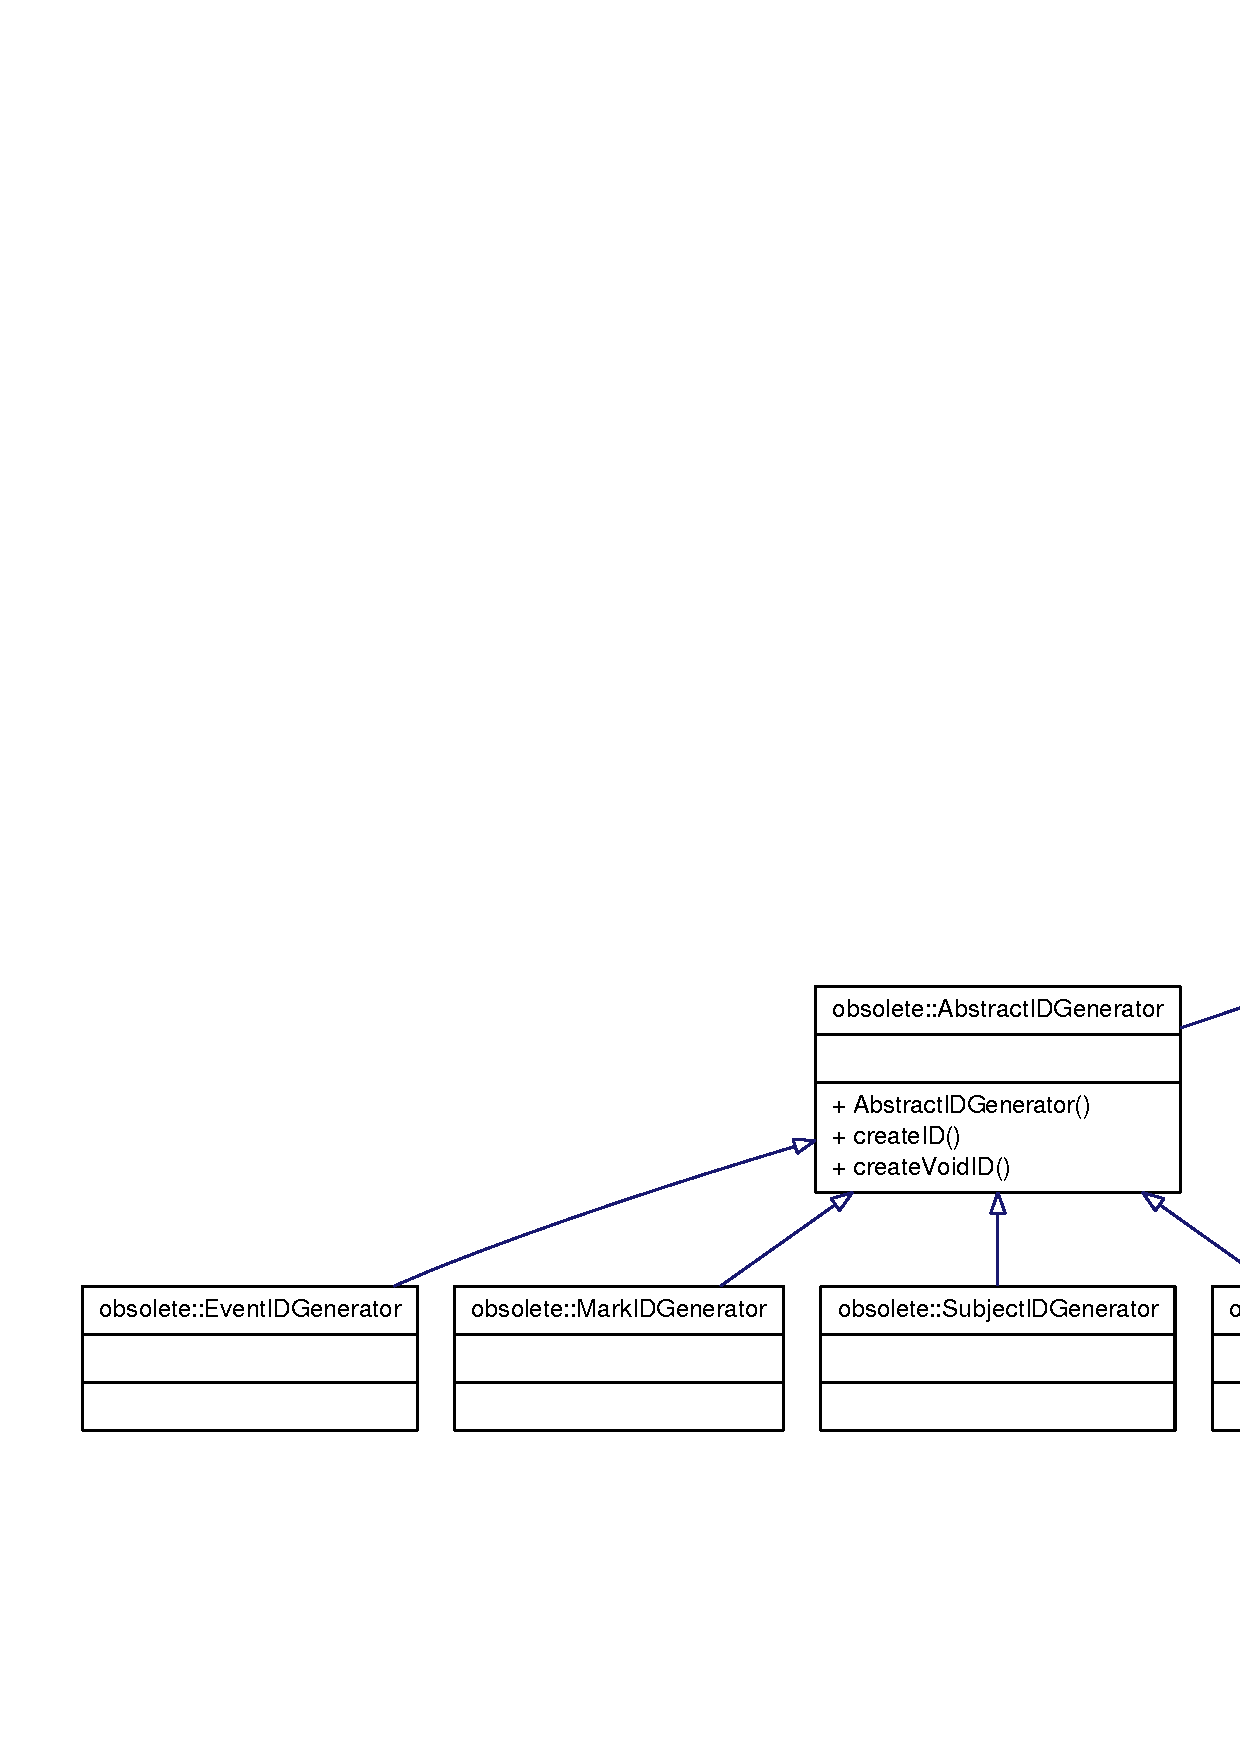
\includegraphics[width=400pt]{classobsolete_1_1AbstractID__inherit__graph}
\end{center}
\end{figure}


Diagram współpracy dla obsolete::AbstractID:\nopagebreak
\begin{figure}[H]
\begin{center}
\leavevmode
\includegraphics[width=166pt]{classobsolete_1_1AbstractID__coll__graph}
\end{center}
\end{figure}
\subsection*{Metody publiczne}
\begin{DoxyCompactItemize}
\item 
\hyperlink{classobsolete_1_1AbstractID_aff6a5e33261e36af0dcf9b38d99f0056}{AbstractID} (uint \hyperlink{classobsolete_1_1ID}{ID}=0)
\begin{DoxyCompactList}\small\item\em Inicjalizuje nowy obiekt. \item\end{DoxyCompactList}\end{DoxyCompactItemize}
\subsection*{Atrybuty chronione}
\begin{DoxyCompactItemize}
\item 
uint \hyperlink{classobsolete_1_1AbstractID_a5f67fa1c7d96085f0ef41193b60b570c}{ID}
\begin{DoxyCompactList}\small\item\em Reprezentowany \hyperlink{classobsolete_1_1ID}{ID}. \item\end{DoxyCompactList}\end{DoxyCompactItemize}
\subsection*{Przyjaciele}
\begin{DoxyCompactItemize}
\item 
QDataStream \& \hyperlink{classobsolete_1_1AbstractID_ae018346f525245975a90a561d3cffccd}{operator$<$$<$} (QDataStream \&stream, const \hyperlink{classobsolete_1_1AbstractID}{AbstractID} \&\hyperlink{classobsolete_1_1ID}{ID})
\begin{DoxyCompactList}\small\item\em Zapisuje dany identyfikator do danego strumienia. \item\end{DoxyCompactList}\item 
QDataStream \& \hyperlink{classobsolete_1_1AbstractID_ae2290b15582443d09db5f4963e546920}{operator$>$$>$} (QDataStream \&stream, \hyperlink{classobsolete_1_1AbstractID}{AbstractID} \&\hyperlink{classobsolete_1_1ID}{ID})
\begin{DoxyCompactList}\small\item\em Odczytuje dany identyfikator z danego strumienia. \item\end{DoxyCompactList}\end{DoxyCompactItemize}


\subsection{Opis szczegółowy}
Klasa bazowa dla wszystkich typów identyfikatorowych. 

Definicja w linii 11 pliku abstractid.h.



\subsection{Dokumentacja konstruktora i destruktora}
\hypertarget{classobsolete_1_1AbstractID_aff6a5e33261e36af0dcf9b38d99f0056}{
\index{obsolete::AbstractID@{obsolete::AbstractID}!AbstractID@{AbstractID}}
\index{AbstractID@{AbstractID}!obsolete::AbstractID@{obsolete::AbstractID}}
\subsubsection[{AbstractID}]{\setlength{\rightskip}{0pt plus 5cm}obsolete::AbstractID::AbstractID (uint {\em ID} = {\ttfamily 0})\hspace{0.3cm}{\ttfamily  \mbox{[}inline\mbox{]}}}}
\label{classobsolete_1_1AbstractID_aff6a5e33261e36af0dcf9b38d99f0056}


Inicjalizuje nowy obiekt. 

Użytkownik powinien użyć metody createdID(). 

Definicja w linii 31 pliku abstractid.h.




\begin{DoxyCode}
31 : ID ( ID ) {}
\end{DoxyCode}




\subsection{Dokumentacja przyjaciół i funkcji związanych}
\hypertarget{classobsolete_1_1AbstractID_ae018346f525245975a90a561d3cffccd}{
\index{obsolete::AbstractID@{obsolete::AbstractID}!operator$<$$<$@{operator$<$$<$}}
\index{operator$<$$<$@{operator$<$$<$}!obsolete::AbstractID@{obsolete::AbstractID}}
\subsubsection[{operator$<$$<$}]{\setlength{\rightskip}{0pt plus 5cm}QDataStream\& operator$<$$<$ (QDataStream \& {\em stream}, \/  const {\bf AbstractID} \& {\em ID})\hspace{0.3cm}{\ttfamily  \mbox{[}friend\mbox{]}}}}
\label{classobsolete_1_1AbstractID_ae018346f525245975a90a561d3cffccd}


Zapisuje dany identyfikator do danego strumienia. 


\begin{DoxyParams}{Parametry}
\item[{\em stream}]Strumień do którego będzie zapisany identyfikator. \item[{\em \hyperlink{classobsolete_1_1ID}{ID}}]Identyfikator który zostanie zapisany. \end{DoxyParams}
\begin{DoxyReturn}{Zwraca}
Ten sam strumień. 
\end{DoxyReturn}
\hypertarget{classobsolete_1_1AbstractID_ae2290b15582443d09db5f4963e546920}{
\index{obsolete::AbstractID@{obsolete::AbstractID}!operator$>$$>$@{operator$>$$>$}}
\index{operator$>$$>$@{operator$>$$>$}!obsolete::AbstractID@{obsolete::AbstractID}}
\subsubsection[{operator$>$$>$}]{\setlength{\rightskip}{0pt plus 5cm}QDataStream\& operator$>$$>$ (QDataStream \& {\em stream}, \/  {\bf AbstractID} \& {\em ID})\hspace{0.3cm}{\ttfamily  \mbox{[}friend\mbox{]}}}}
\label{classobsolete_1_1AbstractID_ae2290b15582443d09db5f4963e546920}


Odczytuje dany identyfikator z danego strumienia. 


\begin{DoxyParams}{Parametry}
\item[{\em stream}]Strumień z którego będzie odczytany identyfikator. \item[{\em \hyperlink{classobsolete_1_1ID}{ID}}]Identyfikator który zostanie zainicjalizowany odczytanymi danymi. \end{DoxyParams}
\begin{DoxyReturn}{Zwraca}
Ten sam strumień. 
\end{DoxyReturn}


\subsection{Dokumentacja atrybutów składowych}
\hypertarget{classobsolete_1_1AbstractID_a5f67fa1c7d96085f0ef41193b60b570c}{
\index{obsolete::AbstractID@{obsolete::AbstractID}!ID@{ID}}
\index{ID@{ID}!obsolete::AbstractID@{obsolete::AbstractID}}
\subsubsection[{ID}]{\setlength{\rightskip}{0pt plus 5cm}uint {\bf obsolete::AbstractID::ID}\hspace{0.3cm}{\ttfamily  \mbox{[}protected\mbox{]}}}}
\label{classobsolete_1_1AbstractID_a5f67fa1c7d96085f0ef41193b60b570c}


Reprezentowany \hyperlink{classobsolete_1_1ID}{ID}. 



Definicja w linii 34 pliku abstractid.h.



Dokumentacja dla tej klasy została wygenerowana z pliku:\begin{DoxyCompactItemize}
\item 
include/obsolete/\hyperlink{abstractid_8h}{abstractid.h}\end{DoxyCompactItemize}

\hypertarget{classobsolete_1_1AbstractIDGenerator}{
\section{Dokumentacja klasy obsolete::AbstractIDGenerator}
\label{classobsolete_1_1AbstractIDGenerator}\index{obsolete::AbstractIDGenerator@{obsolete::AbstractIDGenerator}}
}


Klasa bazowa obiektów-\/generatorów identyfikatorów.  




{\ttfamily \#include $<$abstractidgenerator.h$>$}



Diagram dziedziczenia dla obsolete::AbstractIDGenerator\nopagebreak
\begin{figure}[H]
\begin{center}
\leavevmode
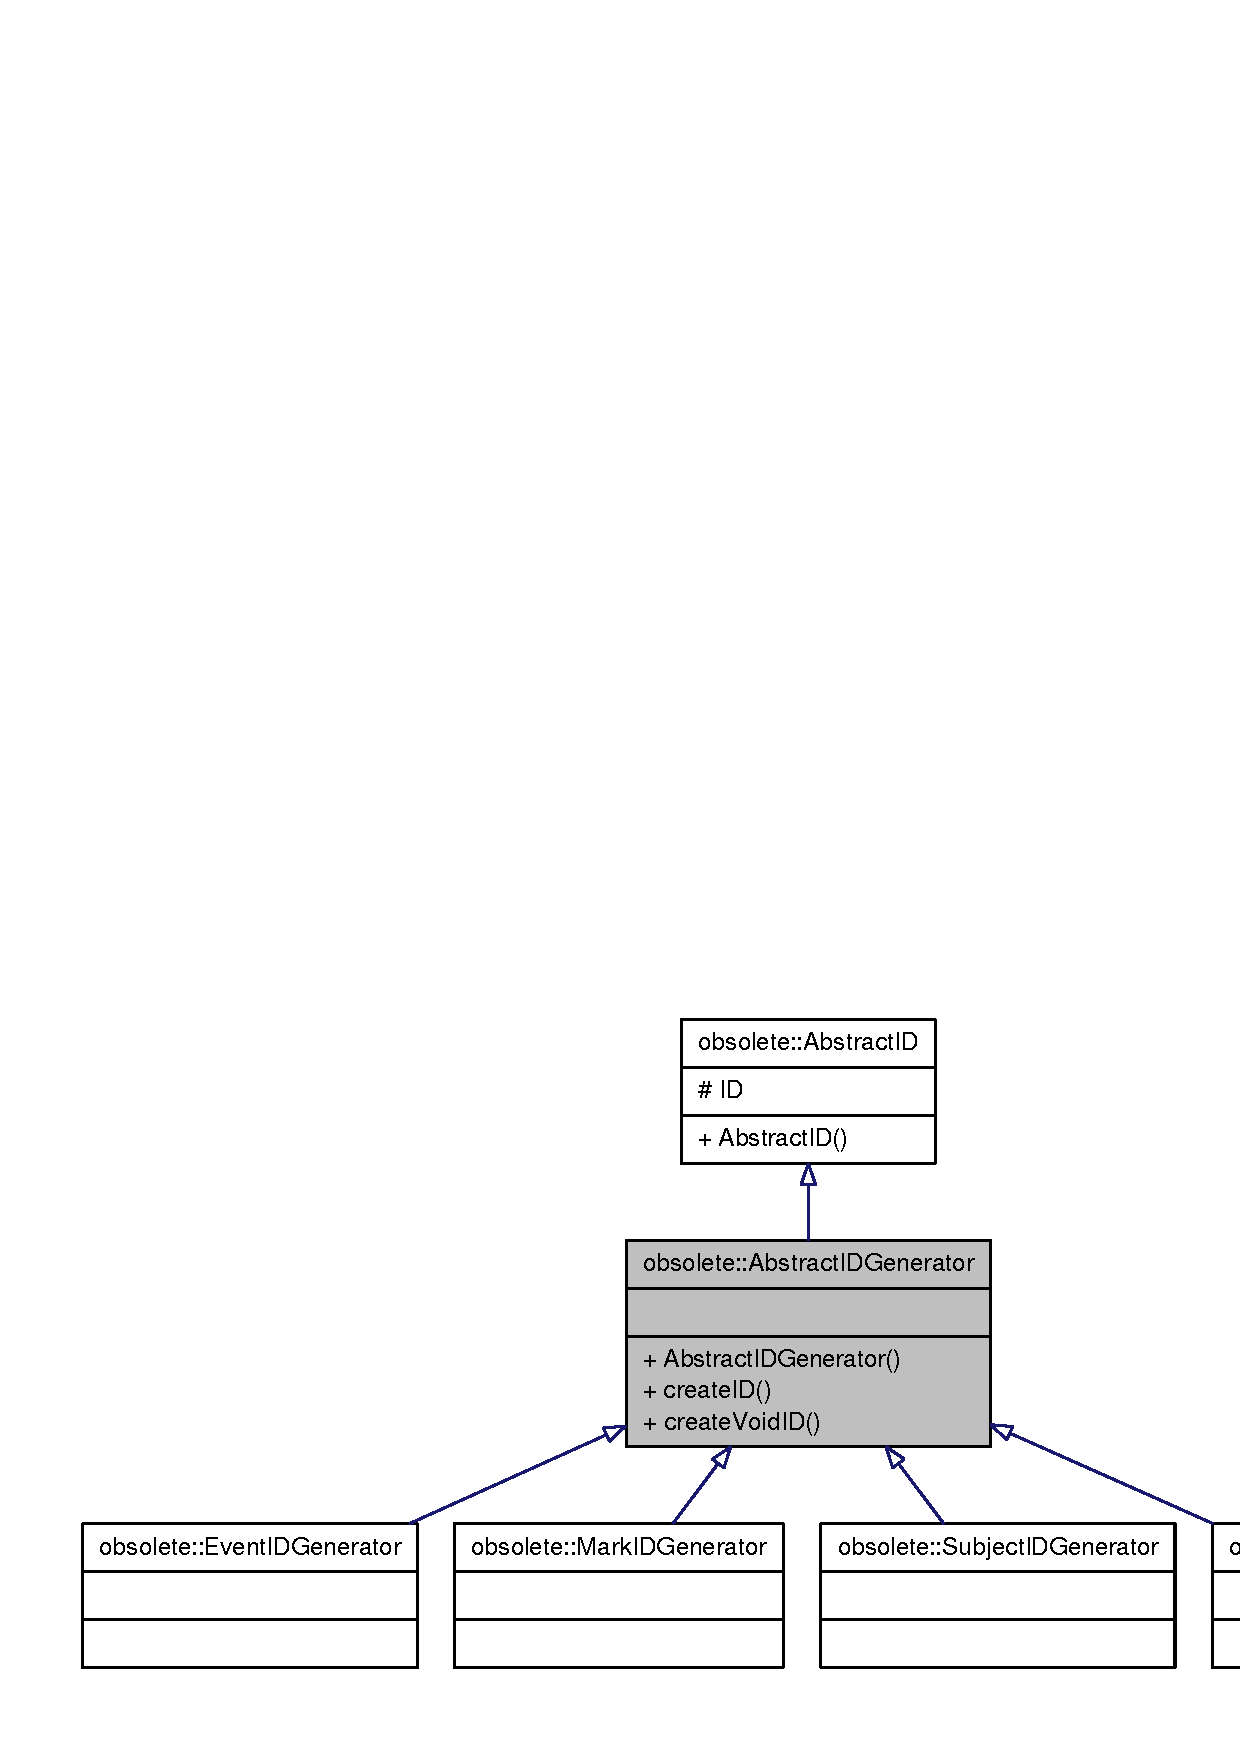
\includegraphics[width=400pt]{classobsolete_1_1AbstractIDGenerator__inherit__graph}
\end{center}
\end{figure}


Diagram współpracy dla obsolete::AbstractIDGenerator:\nopagebreak
\begin{figure}[H]
\begin{center}
\leavevmode
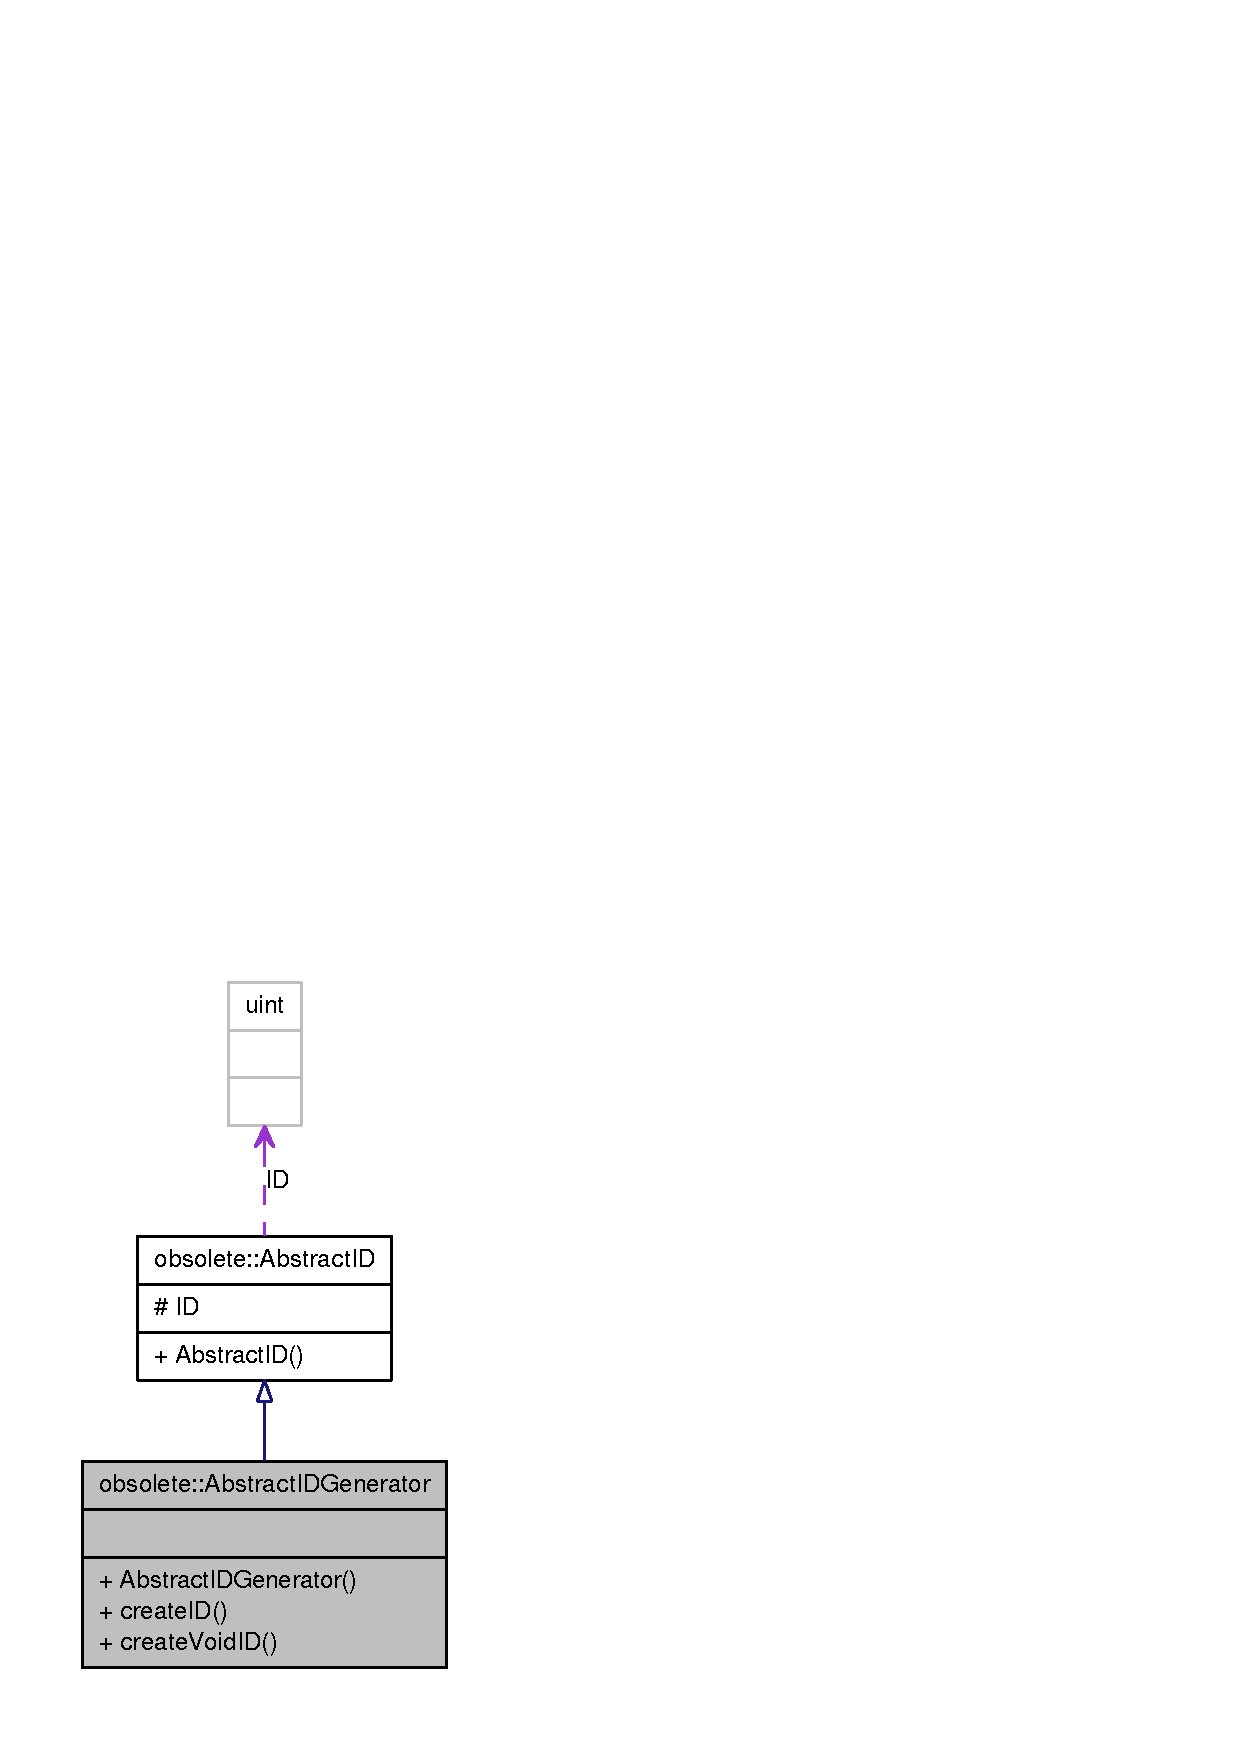
\includegraphics[width=218pt]{classobsolete_1_1AbstractIDGenerator__coll__graph}
\end{center}
\end{figure}
\subsection*{Metody publiczne}
\begin{DoxyCompactItemize}
\item 
\hyperlink{classobsolete_1_1AbstractIDGenerator_a99b8f2659b2f0120f5601789ea89edc1}{AbstractIDGenerator} (uint \hyperlink{classobsolete_1_1ID}{ID}=1)
\begin{DoxyCompactList}\small\item\em Inicjalizuje wartość początkową generatora identyfikatorów. \item\end{DoxyCompactList}\item 
virtual \hyperlink{classobsolete_1_1ID}{ID} \hyperlink{classobsolete_1_1AbstractIDGenerator_a39d2f0147e3a028fef8299770e23db90}{createID} ()
\begin{DoxyCompactList}\small\item\em Tworzy nowy identyfikator. \item\end{DoxyCompactList}\end{DoxyCompactItemize}
\subsection*{Statyczne metody publiczne}
\begin{DoxyCompactItemize}
\item 
static \hyperlink{classobsolete_1_1ID}{ID} \hyperlink{classobsolete_1_1AbstractIDGenerator_a330da88ba80820ca6ce0a29cbbab9e1b}{createVoidID} ()
\begin{DoxyCompactList}\small\item\em Tworzy niezainicjowany identyfikator. \item\end{DoxyCompactList}\end{DoxyCompactItemize}
\subsection*{Atrybuty chronione}
\begin{DoxyCompactItemize}
\item 
uint \hyperlink{classobsolete_1_1AbstractID_a5f67fa1c7d96085f0ef41193b60b570c}{ID}
\begin{DoxyCompactList}\small\item\em Reprezentowany \hyperlink{classobsolete_1_1ID}{ID}. \item\end{DoxyCompactList}\end{DoxyCompactItemize}


\subsection{Opis szczegółowy}
Klasa bazowa obiektów-\/generatorów identyfikatorów. 

Definicja w linii 9 pliku abstractidgenerator.h.



\subsection{Dokumentacja konstruktora i destruktora}
\hypertarget{classobsolete_1_1AbstractIDGenerator_a99b8f2659b2f0120f5601789ea89edc1}{
\index{obsolete::AbstractIDGenerator@{obsolete::AbstractIDGenerator}!AbstractIDGenerator@{AbstractIDGenerator}}
\index{AbstractIDGenerator@{AbstractIDGenerator}!obsolete::AbstractIDGenerator@{obsolete::AbstractIDGenerator}}
\subsubsection[{AbstractIDGenerator}]{\setlength{\rightskip}{0pt plus 5cm}obsolete::AbstractIDGenerator::AbstractIDGenerator (uint {\em ID} = {\ttfamily 1})\hspace{0.3cm}{\ttfamily  \mbox{[}inline\mbox{]}}}}
\label{classobsolete_1_1AbstractIDGenerator_a99b8f2659b2f0120f5601789ea89edc1}


Inicjalizuje wartość początkową generatora identyfikatorów. 



Definicja w linii 8 pliku abstractidgenerator.h.



\subsection{Dokumentacja funkcji składowych}
\hypertarget{classobsolete_1_1AbstractIDGenerator_a39d2f0147e3a028fef8299770e23db90}{
\index{obsolete::AbstractIDGenerator@{obsolete::AbstractIDGenerator}!createID@{createID}}
\index{createID@{createID}!obsolete::AbstractIDGenerator@{obsolete::AbstractIDGenerator}}
\subsubsection[{createID}]{\setlength{\rightskip}{0pt plus 5cm}virtual {\bf ID} obsolete::AbstractIDGenerator::createID ()\hspace{0.3cm}{\ttfamily  \mbox{[}virtual\mbox{]}}}}
\label{classobsolete_1_1AbstractIDGenerator_a39d2f0147e3a028fef8299770e23db90}


Tworzy nowy identyfikator. 

\hypertarget{classobsolete_1_1AbstractIDGenerator_a330da88ba80820ca6ce0a29cbbab9e1b}{
\index{obsolete::AbstractIDGenerator@{obsolete::AbstractIDGenerator}!createVoidID@{createVoidID}}
\index{createVoidID@{createVoidID}!obsolete::AbstractIDGenerator@{obsolete::AbstractIDGenerator}}
\subsubsection[{createVoidID}]{\setlength{\rightskip}{0pt plus 5cm}static {\bf ID} obsolete::AbstractIDGenerator::createVoidID ()\hspace{0.3cm}{\ttfamily  \mbox{[}static\mbox{]}}}}
\label{classobsolete_1_1AbstractIDGenerator_a330da88ba80820ca6ce0a29cbbab9e1b}


Tworzy niezainicjowany identyfikator. 



\subsection{Dokumentacja atrybutów składowych}
\hypertarget{classobsolete_1_1AbstractID_a5f67fa1c7d96085f0ef41193b60b570c}{
\index{obsolete::AbstractIDGenerator@{obsolete::AbstractIDGenerator}!ID@{ID}}
\index{ID@{ID}!obsolete::AbstractIDGenerator@{obsolete::AbstractIDGenerator}}
\subsubsection[{ID}]{\setlength{\rightskip}{0pt plus 5cm}uint {\bf obsolete::AbstractID::ID}\hspace{0.3cm}{\ttfamily  \mbox{[}protected, inherited\mbox{]}}}}
\label{classobsolete_1_1AbstractID_a5f67fa1c7d96085f0ef41193b60b570c}


Reprezentowany \hyperlink{classobsolete_1_1ID}{ID}. 



Definicja w linii 34 pliku abstractid.h.



Dokumentacja dla tej klasy została wygenerowana z pliku:\begin{DoxyCompactItemize}
\item 
include/obsolete/\hyperlink{abstractidgenerator_8h}{abstractidgenerator.h}\end{DoxyCompactItemize}

\hypertarget{classobsolete_1_1AbstractIncrementalID}{
\section{Dokumentacja klasy obsolete::AbstractIncrementalID}
\label{classobsolete_1_1AbstractIncrementalID}\index{obsolete::AbstractIncrementalID@{obsolete::AbstractIncrementalID}}
}


Podstawa dla wszystkich klas identyfikatorów automatycznych.  




{\ttfamily \#include $<$abstractincrementalid.h$>$}



Diagram dziedziczenia dla obsolete::AbstractIncrementalID\nopagebreak
\begin{figure}[H]
\begin{center}
\leavevmode
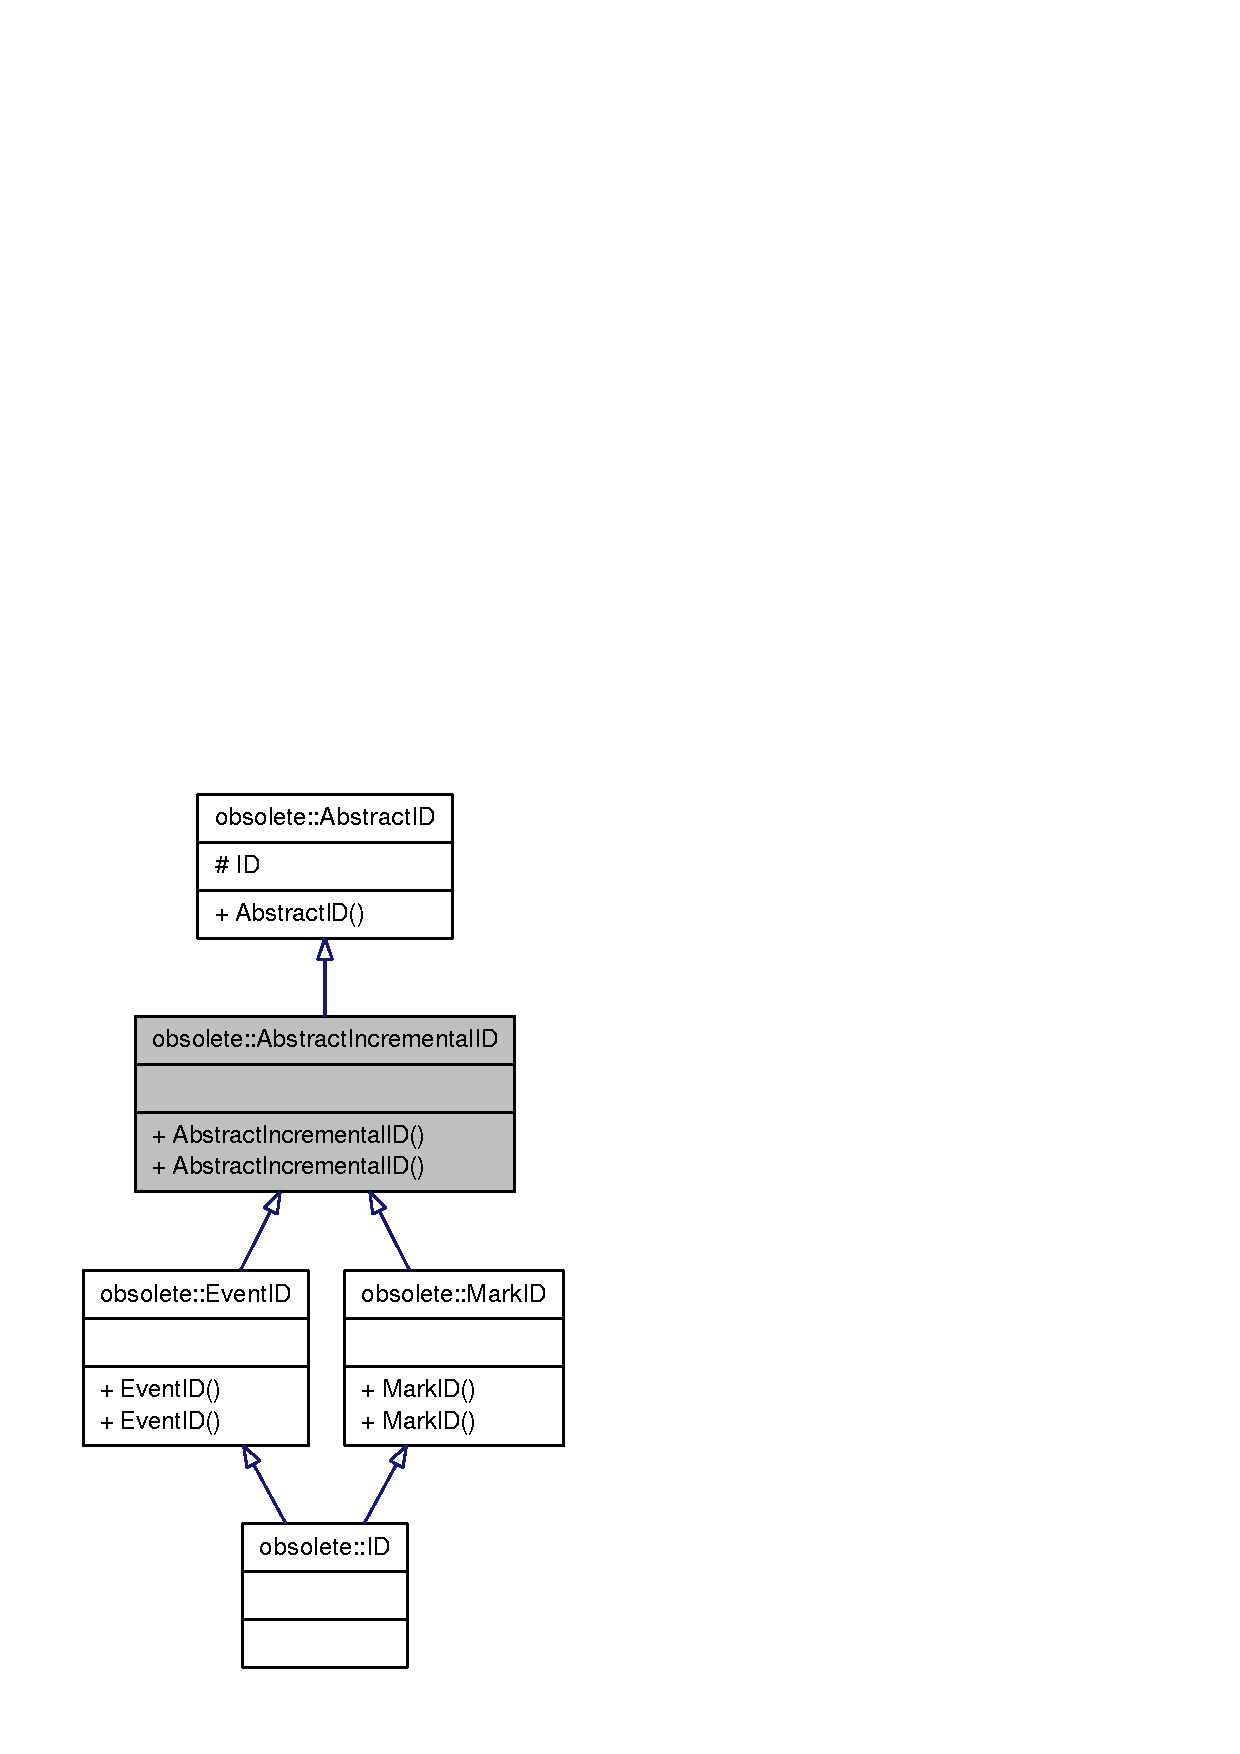
\includegraphics[height=400pt]{classobsolete_1_1AbstractIncrementalID__inherit__graph}
\end{center}
\end{figure}


Diagram współpracy dla obsolete::AbstractIncrementalID:\nopagebreak
\begin{figure}[H]
\begin{center}
\leavevmode
\includegraphics[width=226pt]{classobsolete_1_1AbstractIncrementalID__coll__graph}
\end{center}
\end{figure}
\subsection*{Metody publiczne}
\begin{DoxyCompactItemize}
\item 
\hyperlink{classobsolete_1_1AbstractIncrementalID_a7977c3993208ff1ff91b36bbc7aed925}{AbstractIncrementalID} (uint \hyperlink{classobsolete_1_1ID}{ID})
\begin{DoxyCompactList}\small\item\em Wykorzystuje konstruktor klasy nadrzędnej. \item\end{DoxyCompactList}\item 
\hyperlink{classobsolete_1_1AbstractIncrementalID_a6f379264ad7fa66c1a4be8d14214497b}{AbstractIncrementalID} ()
\begin{DoxyCompactList}\small\item\em Pozwalam również na tworzenie niezainicjalizowanych obiektów. \item\end{DoxyCompactList}\end{DoxyCompactItemize}
\subsection*{Atrybuty chronione}
\begin{DoxyCompactItemize}
\item 
uint \hyperlink{classobsolete_1_1AbstractID_a5f67fa1c7d96085f0ef41193b60b570c}{ID}
\begin{DoxyCompactList}\small\item\em Reprezentowany \hyperlink{classobsolete_1_1ID}{ID}. \item\end{DoxyCompactList}\end{DoxyCompactItemize}


\subsection{Opis szczegółowy}
Podstawa dla wszystkich klas identyfikatorów automatycznych. 

Definicja w linii 10 pliku abstractincrementalid.h.



\subsection{Dokumentacja konstruktora i destruktora}
\hypertarget{classobsolete_1_1AbstractIncrementalID_a7977c3993208ff1ff91b36bbc7aed925}{
\index{obsolete::AbstractIncrementalID@{obsolete::AbstractIncrementalID}!AbstractIncrementalID@{AbstractIncrementalID}}
\index{AbstractIncrementalID@{AbstractIncrementalID}!obsolete::AbstractIncrementalID@{obsolete::AbstractIncrementalID}}
\subsubsection[{AbstractIncrementalID}]{\setlength{\rightskip}{0pt plus 5cm}obsolete::AbstractIncrementalID::AbstractIncrementalID (uint {\em ID})\hspace{0.3cm}{\ttfamily  \mbox{[}inline\mbox{]}}}}
\label{classobsolete_1_1AbstractIncrementalID_a7977c3993208ff1ff91b36bbc7aed925}


Wykorzystuje konstruktor klasy nadrzędnej. 



Definicja w linii 13 pliku abstractincrementalid.h.

\hypertarget{classobsolete_1_1AbstractIncrementalID_a6f379264ad7fa66c1a4be8d14214497b}{
\index{obsolete::AbstractIncrementalID@{obsolete::AbstractIncrementalID}!AbstractIncrementalID@{AbstractIncrementalID}}
\index{AbstractIncrementalID@{AbstractIncrementalID}!obsolete::AbstractIncrementalID@{obsolete::AbstractIncrementalID}}
\subsubsection[{AbstractIncrementalID}]{\setlength{\rightskip}{0pt plus 5cm}obsolete::AbstractIncrementalID::AbstractIncrementalID ()\hspace{0.3cm}{\ttfamily  \mbox{[}inline\mbox{]}}}}
\label{classobsolete_1_1AbstractIncrementalID_a6f379264ad7fa66c1a4be8d14214497b}


Pozwalam również na tworzenie niezainicjalizowanych obiektów. 



Definicja w linii 14 pliku abstractincrementalid.h.



\subsection{Dokumentacja atrybutów składowych}
\hypertarget{classobsolete_1_1AbstractID_a5f67fa1c7d96085f0ef41193b60b570c}{
\index{obsolete::AbstractIncrementalID@{obsolete::AbstractIncrementalID}!ID@{ID}}
\index{ID@{ID}!obsolete::AbstractIncrementalID@{obsolete::AbstractIncrementalID}}
\subsubsection[{ID}]{\setlength{\rightskip}{0pt plus 5cm}uint {\bf obsolete::AbstractID::ID}\hspace{0.3cm}{\ttfamily  \mbox{[}protected, inherited\mbox{]}}}}
\label{classobsolete_1_1AbstractID_a5f67fa1c7d96085f0ef41193b60b570c}


Reprezentowany \hyperlink{classobsolete_1_1ID}{ID}. 



Definicja w linii 34 pliku abstractid.h.



Dokumentacja dla tej klasy została wygenerowana z pliku:\begin{DoxyCompactItemize}
\item 
include/obsolete/\hyperlink{abstractincrementalid_8h}{abstractincrementalid.h}\end{DoxyCompactItemize}

\hypertarget{classobsolete_1_1AbstractReservedID}{
\section{Dokumentacja klasy obsolete::AbstractReservedID}
\label{classobsolete_1_1AbstractReservedID}\index{obsolete::AbstractReservedID@{obsolete::AbstractReservedID}}
}


Klasa reprezentująca identyfikatory rezerwowane z góry.  




{\ttfamily \#include $<$abstractreservedid.h$>$}



Diagram dziedziczenia dla obsolete::AbstractReservedID\nopagebreak
\begin{figure}[H]
\begin{center}
\leavevmode
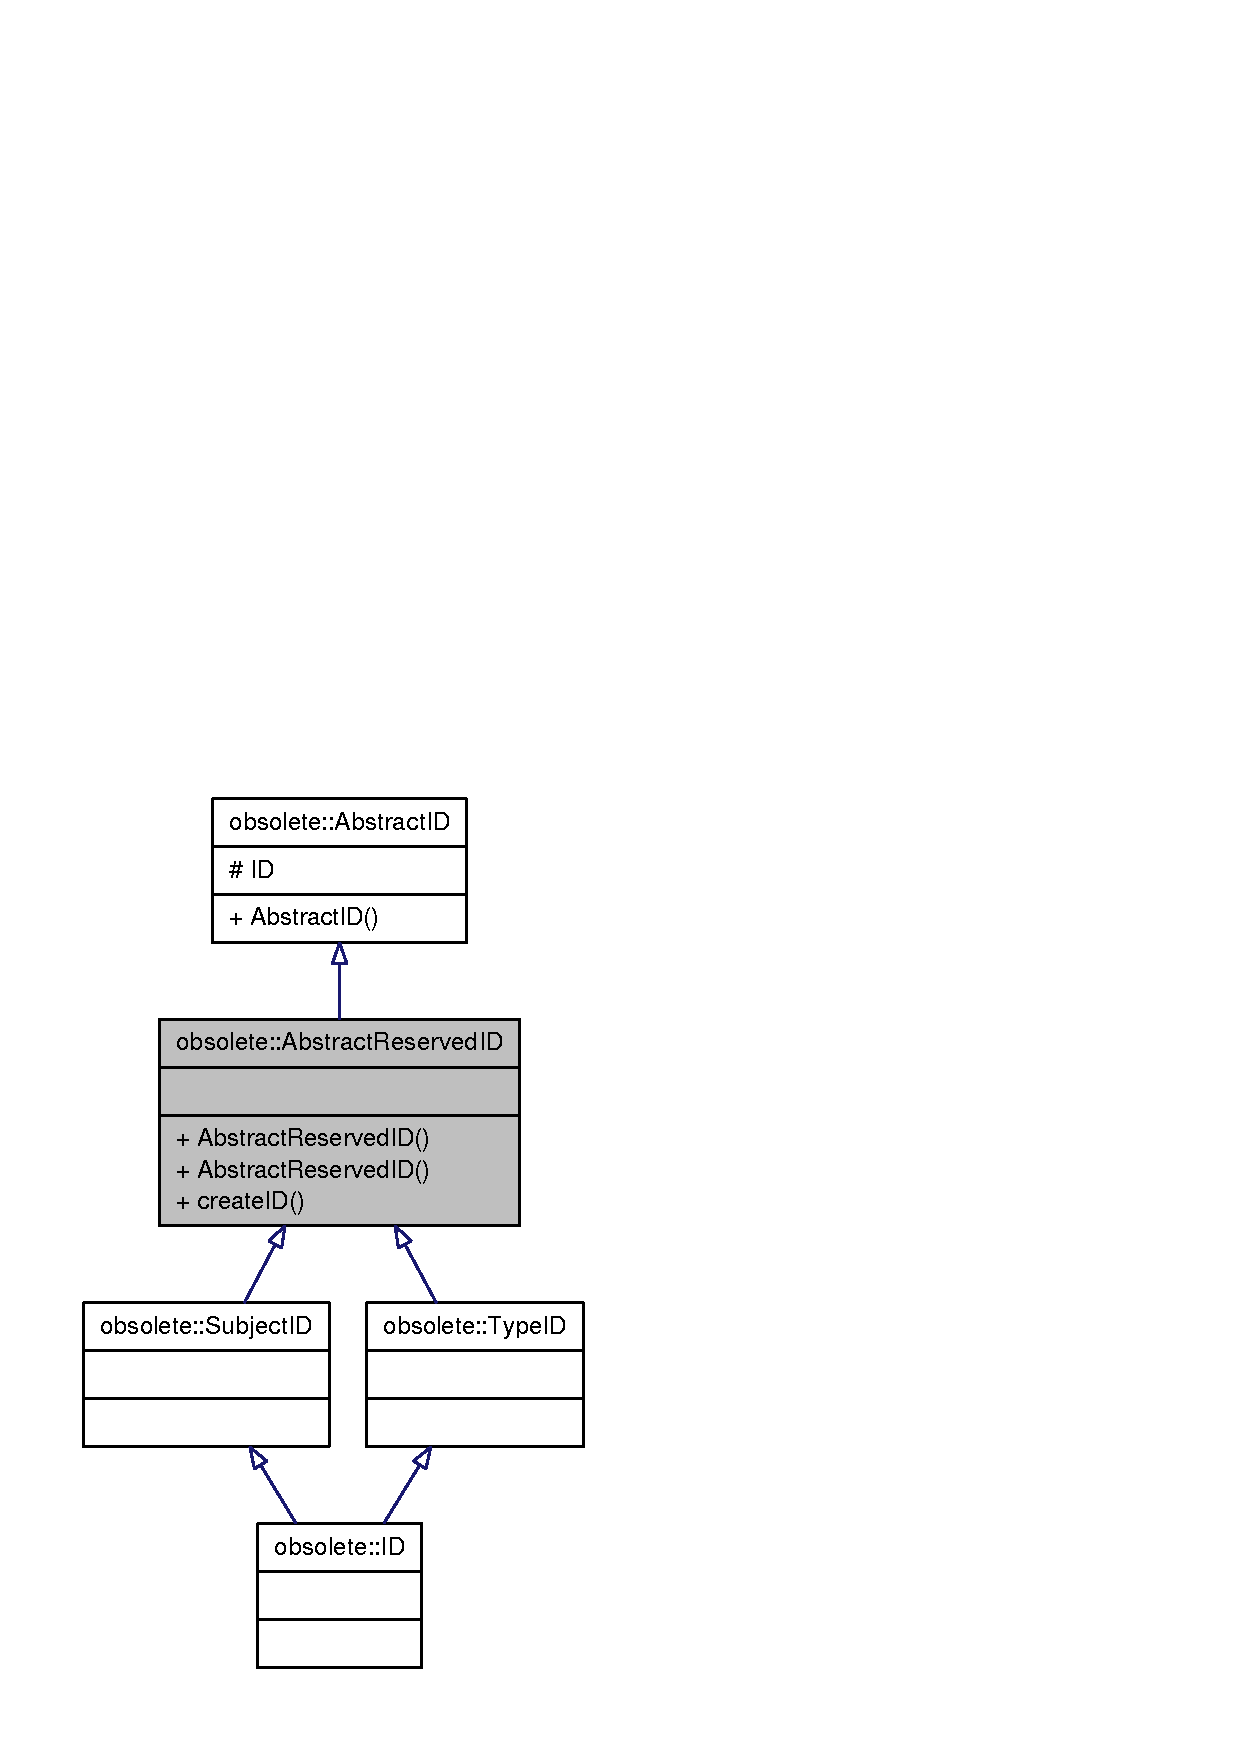
\includegraphics[height=400pt]{classobsolete_1_1AbstractReservedID__inherit__graph}
\end{center}
\end{figure}


Diagram współpracy dla obsolete::AbstractReservedID:\nopagebreak
\begin{figure}[H]
\begin{center}
\leavevmode
\includegraphics[width=216pt]{classobsolete_1_1AbstractReservedID__coll__graph}
\end{center}
\end{figure}
\subsection*{Metody publiczne}
\begin{DoxyCompactItemize}
\item 
\hyperlink{classobsolete_1_1AbstractReservedID_ad24b4475da6154fdc7d5d146a8fb311f}{AbstractReservedID} (uint \hyperlink{classobsolete_1_1ID}{ID})
\begin{DoxyCompactList}\small\item\em Wykorzystuje konstruktor klasy nadrzędnej. \item\end{DoxyCompactList}\item 
\hyperlink{classobsolete_1_1AbstractReservedID_ae01ec9522e9f8e7bbf28defe15266c2e}{AbstractReservedID} ()
\begin{DoxyCompactList}\small\item\em Pozwalam również na tworzenie niezainicjalizowanych obiektów. \item\end{DoxyCompactList}\end{DoxyCompactItemize}
\subsection*{Statyczne metody publiczne}
\begin{DoxyCompactItemize}
\item 
static \hyperlink{classobsolete_1_1AbstractReservedID}{AbstractReservedID} \hyperlink{classobsolete_1_1AbstractReservedID_a38fa00bf6097ab9cff285c8480c8097e}{createID} (uint \hyperlink{classobsolete_1_1ID}{ID})
\begin{DoxyCompactList}\small\item\em Opakowuje numer porządkowy zadaną liczbą. \item\end{DoxyCompactList}\end{DoxyCompactItemize}
\subsection*{Atrybuty chronione}
\begin{DoxyCompactItemize}
\item 
uint \hyperlink{classobsolete_1_1AbstractID_a5f67fa1c7d96085f0ef41193b60b570c}{ID}
\begin{DoxyCompactList}\small\item\em Reprezentowany \hyperlink{classobsolete_1_1ID}{ID}. \item\end{DoxyCompactList}\end{DoxyCompactItemize}


\subsection{Opis szczegółowy}
Klasa reprezentująca identyfikatory rezerwowane z góry. (coś w stylu haszowanie doskonałe) 

Definicja w linii 10 pliku abstractreservedid.h.



\subsection{Dokumentacja konstruktora i destruktora}
\hypertarget{classobsolete_1_1AbstractReservedID_ad24b4475da6154fdc7d5d146a8fb311f}{
\index{obsolete::AbstractReservedID@{obsolete::AbstractReservedID}!AbstractReservedID@{AbstractReservedID}}
\index{AbstractReservedID@{AbstractReservedID}!obsolete::AbstractReservedID@{obsolete::AbstractReservedID}}
\subsubsection[{AbstractReservedID}]{\setlength{\rightskip}{0pt plus 5cm}obsolete::AbstractReservedID::AbstractReservedID (uint {\em ID})\hspace{0.3cm}{\ttfamily  \mbox{[}inline\mbox{]}}}}
\label{classobsolete_1_1AbstractReservedID_ad24b4475da6154fdc7d5d146a8fb311f}


Wykorzystuje konstruktor klasy nadrzędnej. 



Definicja w linii 13 pliku abstractreservedid.h.

\hypertarget{classobsolete_1_1AbstractReservedID_ae01ec9522e9f8e7bbf28defe15266c2e}{
\index{obsolete::AbstractReservedID@{obsolete::AbstractReservedID}!AbstractReservedID@{AbstractReservedID}}
\index{AbstractReservedID@{AbstractReservedID}!obsolete::AbstractReservedID@{obsolete::AbstractReservedID}}
\subsubsection[{AbstractReservedID}]{\setlength{\rightskip}{0pt plus 5cm}obsolete::AbstractReservedID::AbstractReservedID ()\hspace{0.3cm}{\ttfamily  \mbox{[}inline\mbox{]}}}}
\label{classobsolete_1_1AbstractReservedID_ae01ec9522e9f8e7bbf28defe15266c2e}


Pozwalam również na tworzenie niezainicjalizowanych obiektów. 



Definicja w linii 14 pliku abstractreservedid.h.



\subsection{Dokumentacja funkcji składowych}
\hypertarget{classobsolete_1_1AbstractReservedID_a38fa00bf6097ab9cff285c8480c8097e}{
\index{obsolete::AbstractReservedID@{obsolete::AbstractReservedID}!createID@{createID}}
\index{createID@{createID}!obsolete::AbstractReservedID@{obsolete::AbstractReservedID}}
\subsubsection[{createID}]{\setlength{\rightskip}{0pt plus 5cm}static {\bf AbstractReservedID} obsolete::AbstractReservedID::createID (uint {\em ID})\hspace{0.3cm}{\ttfamily  \mbox{[}inline, static\mbox{]}}}}
\label{classobsolete_1_1AbstractReservedID_a38fa00bf6097ab9cff285c8480c8097e}


Opakowuje numer porządkowy zadaną liczbą. 



\subsection{Dokumentacja atrybutów składowych}
\hypertarget{classobsolete_1_1AbstractID_a5f67fa1c7d96085f0ef41193b60b570c}{
\index{obsolete::AbstractReservedID@{obsolete::AbstractReservedID}!ID@{ID}}
\index{ID@{ID}!obsolete::AbstractReservedID@{obsolete::AbstractReservedID}}
\subsubsection[{ID}]{\setlength{\rightskip}{0pt plus 5cm}uint {\bf obsolete::AbstractID::ID}\hspace{0.3cm}{\ttfamily  \mbox{[}protected, inherited\mbox{]}}}}
\label{classobsolete_1_1AbstractID_a5f67fa1c7d96085f0ef41193b60b570c}


Reprezentowany \hyperlink{classobsolete_1_1ID}{ID}. 



Definicja w linii 34 pliku abstractid.h.



Dokumentacja dla tej klasy została wygenerowana z pliku:\begin{DoxyCompactItemize}
\item 
include/obsolete/\hyperlink{abstractreservedid_8h}{abstractreservedid.h}\end{DoxyCompactItemize}

\hypertarget{classEvent}{
\section{Dokumentacja klasy Event}
\label{classEvent}\index{Event@{Event}}
}


Reprezentuje zdarzenie w postaci zdefiniowanej przez użytkownika.  




{\ttfamily \#include $<$event.h$>$}



Diagram współpracy dla Event:\nopagebreak
\begin{figure}[H]
\begin{center}
\leavevmode
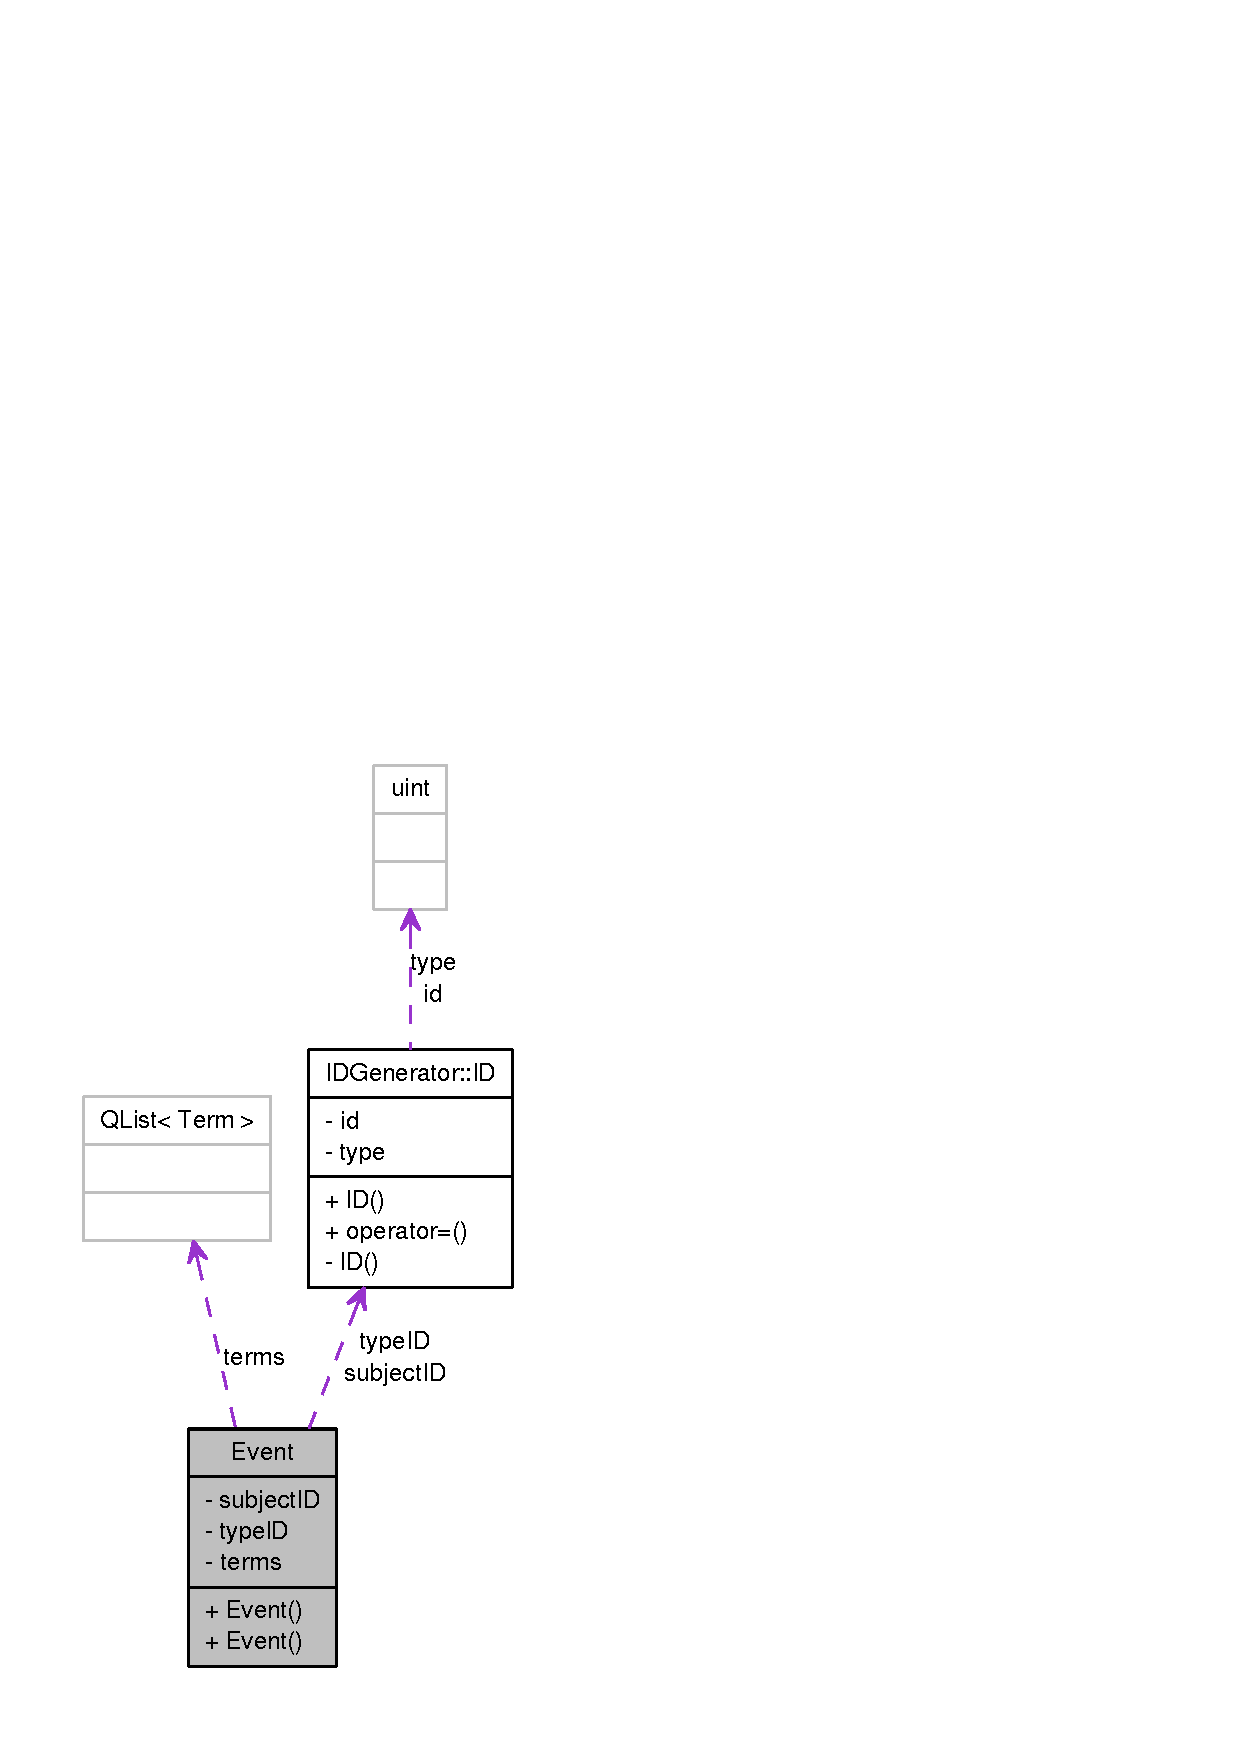
\includegraphics[height=400pt]{classEvent__coll__graph}
\end{center}
\end{figure}
\subsection*{Metody publiczne}
\begin{DoxyCompactItemize}
\item 
\hyperlink{classEvent_acd3992dc833e31573a209ba44910b57f}{Event} (\hyperlink{classIDGenerator_1_1ID}{IDGenerator::ID} \hyperlink{classEvent_a584a3fce37eaa31ee45c202a538f59b6}{subjectID}, \hyperlink{classIDGenerator_1_1ID}{IDGenerator::ID} \hyperlink{classEvent_a8abdf6e037043e6d6d761de593d33807}{typeID}, QList$<$ \hyperlink{classTerm}{Term} $>$ term=QList$<$ \hyperlink{classTerm}{Term} $>$())
\begin{DoxyCompactList}\small\item\em Inicjalizuje dane wydarzenie niezbędnymi informacjami. \item\end{DoxyCompactList}\item 
\hyperlink{classEvent_a5a40dd4708297f7031e29b39e039ae10}{Event} ()
\begin{DoxyCompactList}\small\item\em Umożliwia tworzenie niezainicjalizowanych obiektów. \item\end{DoxyCompactList}\end{DoxyCompactItemize}
\subsection*{Atrybuty prywatne}
\begin{DoxyCompactItemize}
\item 
\hyperlink{classIDGenerator_1_1ID}{IDGenerator::ID} \hyperlink{classEvent_a584a3fce37eaa31ee45c202a538f59b6}{subjectID}
\begin{DoxyCompactList}\small\item\em Identyfikator przedmiotu skojarzonego z wydarzeniem. \item\end{DoxyCompactList}\item 
\hyperlink{classIDGenerator_1_1ID}{IDGenerator::ID} \hyperlink{classEvent_a8abdf6e037043e6d6d761de593d33807}{typeID}
\begin{DoxyCompactList}\small\item\em Identyfikator typu wydarzenia. \item\end{DoxyCompactList}\item 
QList$<$ \hyperlink{classTerm}{Term} $>$ \hyperlink{classEvent_aff6cf909022d62edc3b633281d3121a6}{terms}
\begin{DoxyCompactList}\small\item\em Lista terminów danego wydarzenia. \item\end{DoxyCompactList}\end{DoxyCompactItemize}
\subsection*{Przyjaciele}
\begin{DoxyCompactItemize}
\item 
QDataStream \& \hyperlink{classEvent_a62e8730ab4dc16e3d456b527a12635b3}{operator$<$$<$} (QDataStream \&stream, const \hyperlink{classEvent}{Event} \&event)
\begin{DoxyCompactList}\small\item\em Zapisuje informacje o danym wydarzeniu do danego strumienia. \item\end{DoxyCompactList}\item 
QDataStream \& \hyperlink{classEvent_a055427e98ad131966edb6fb652add004}{operator$>$$>$} (QDataStream \&stream, \hyperlink{classEvent}{Event} \&event)
\begin{DoxyCompactList}\small\item\em Odczytuje informacje o danym wydarzeniu z danego strumienia. \item\end{DoxyCompactList}\end{DoxyCompactItemize}


\subsection{Opis szczegółowy}
Reprezentuje zdarzenie w postaci zdefiniowanej przez użytkownika. Posiada określony typ (zdefiniowany przez użytkownika z dostępnych możliwości (zdefiniowanych przez użytkownika)). Powiązane z terminami.

Pozwala ustawić ocenę. 

Definicja w linii 15 pliku event.h.



\subsection{Dokumentacja konstruktora i destruktora}
\hypertarget{classEvent_acd3992dc833e31573a209ba44910b57f}{
\index{Event@{Event}!Event@{Event}}
\index{Event@{Event}!Event@{Event}}
\subsubsection[{Event}]{\setlength{\rightskip}{0pt plus 5cm}Event::Event ({\bf IDGenerator::ID} {\em subjectID}, \/  {\bf IDGenerator::ID} {\em typeID}, \/  QList$<$ {\bf Term} $>$ {\em term} = {\ttfamily QList$<${\bf Term}$>$()})\hspace{0.3cm}{\ttfamily  \mbox{[}inline\mbox{]}}}}
\label{classEvent_acd3992dc833e31573a209ba44910b57f}


Inicjalizuje dane wydarzenie niezbędnymi informacjami. 


\begin{DoxyParams}{Parametry}
\item[{\em subjectID}]Identyfikator przedmiotu związanego z wydarzeniem \item[{\em typeID}]Identyfikator typu wydarzenia \item[{\em term}]Lista terminów tego wydarzenia. Może być pusta. \end{DoxyParams}


Definicja w linii 30 pliku event.h.




\begin{DoxyCode}
31 :\end{DoxyCode}


\hypertarget{classEvent_a5a40dd4708297f7031e29b39e039ae10}{
\index{Event@{Event}!Event@{Event}}
\index{Event@{Event}!Event@{Event}}
\subsubsection[{Event}]{\setlength{\rightskip}{0pt plus 5cm}Event::Event ()\hspace{0.3cm}{\ttfamily  \mbox{[}inline\mbox{]}}}}
\label{classEvent_a5a40dd4708297f7031e29b39e039ae10}


Umożliwia tworzenie niezainicjalizowanych obiektów. 



Definicja w linii 33 pliku event.h.



\subsection{Dokumentacja przyjaciół i funkcji związanych}
\hypertarget{classEvent_a62e8730ab4dc16e3d456b527a12635b3}{
\index{Event@{Event}!operator$<$$<$@{operator$<$$<$}}
\index{operator$<$$<$@{operator$<$$<$}!Event@{Event}}
\subsubsection[{operator$<$$<$}]{\setlength{\rightskip}{0pt plus 5cm}QDataStream\& operator$<$$<$ (QDataStream \& {\em stream}, \/  const {\bf Event} \& {\em event})\hspace{0.3cm}{\ttfamily  \mbox{[}friend\mbox{]}}}}
\label{classEvent_a62e8730ab4dc16e3d456b527a12635b3}


Zapisuje informacje o danym wydarzeniu do danego strumienia. 


\begin{DoxyParams}{Parametry}
\item[{\em stream}]Strumień do którego będą zapisywane dane. \item[{\em event}]Wydarzenie które będzie zapisywane. \end{DoxyParams}
\begin{DoxyReturn}{Zwraca}
Ten sam strumień. 
\end{DoxyReturn}


Definicja w linii 3 pliku event.cpp.




\begin{DoxyCode}
4 {
5     return stream<<event.subjectID<<event.typeID<<event.terms;
6 }
\end{DoxyCode}


\hypertarget{classEvent_a055427e98ad131966edb6fb652add004}{
\index{Event@{Event}!operator$>$$>$@{operator$>$$>$}}
\index{operator$>$$>$@{operator$>$$>$}!Event@{Event}}
\subsubsection[{operator$>$$>$}]{\setlength{\rightskip}{0pt plus 5cm}QDataStream\& operator$>$$>$ (QDataStream \& {\em stream}, \/  {\bf Event} \& {\em event})\hspace{0.3cm}{\ttfamily  \mbox{[}friend\mbox{]}}}}
\label{classEvent_a055427e98ad131966edb6fb652add004}


Odczytuje informacje o danym wydarzeniu z danego strumienia. 


\begin{DoxyParams}{Parametry}
\item[{\em stream}]Strumień z którego będą odczytywane dane. \item[{\em event}]Wydarzenie które zostanie zainicjalizowane wczytanymi danymi. \end{DoxyParams}
\begin{DoxyReturn}{Zwraca}
Ten sam strumień. 
\end{DoxyReturn}


Definicja w linii 8 pliku event.cpp.




\begin{DoxyCode}
9 {
10     return stream>>event.subjectID<<event.typeID<<event.terms;
11 }
\end{DoxyCode}




\subsection{Dokumentacja atrybutów składowych}
\hypertarget{classEvent_a584a3fce37eaa31ee45c202a538f59b6}{
\index{Event@{Event}!subjectID@{subjectID}}
\index{subjectID@{subjectID}!Event@{Event}}
\subsubsection[{subjectID}]{\setlength{\rightskip}{0pt plus 5cm}{\bf IDGenerator::ID} {\bf Event::subjectID}\hspace{0.3cm}{\ttfamily  \mbox{[}private\mbox{]}}}}
\label{classEvent_a584a3fce37eaa31ee45c202a538f59b6}


Identyfikator przedmiotu skojarzonego z wydarzeniem. 



Definicja w linii 35 pliku event.h.

\hypertarget{classEvent_aff6cf909022d62edc3b633281d3121a6}{
\index{Event@{Event}!terms@{terms}}
\index{terms@{terms}!Event@{Event}}
\subsubsection[{terms}]{\setlength{\rightskip}{0pt plus 5cm}QList$<${\bf Term}$>$ {\bf Event::terms}\hspace{0.3cm}{\ttfamily  \mbox{[}private\mbox{]}}}}
\label{classEvent_aff6cf909022d62edc3b633281d3121a6}


Lista terminów danego wydarzenia. 



Definicja w linii 37 pliku event.h.

\hypertarget{classEvent_a8abdf6e037043e6d6d761de593d33807}{
\index{Event@{Event}!typeID@{typeID}}
\index{typeID@{typeID}!Event@{Event}}
\subsubsection[{typeID}]{\setlength{\rightskip}{0pt plus 5cm}{\bf IDGenerator::ID} {\bf Event::typeID}\hspace{0.3cm}{\ttfamily  \mbox{[}private\mbox{]}}}}
\label{classEvent_a8abdf6e037043e6d6d761de593d33807}


Identyfikator typu wydarzenia. 



Definicja w linii 36 pliku event.h.



Dokumentacja dla tej klasy została wygenerowana z pliku:\begin{DoxyCompactItemize}
\item 
include/\hyperlink{event_8h}{event.h}\end{DoxyCompactItemize}

\hypertarget{classobsolete_1_1EventID}{
\section{Dokumentacja klasy obsolete::EventID}
\label{classobsolete_1_1EventID}\index{obsolete::EventID@{obsolete::EventID}}
}


Klasa reprezentująca identyfikator zdarzenia.  




{\ttfamily \#include $<$eventid.h$>$}



Diagram dziedziczenia dla obsolete::EventID\nopagebreak
\begin{figure}[H]
\begin{center}
\leavevmode
\includegraphics[height=400pt]{classobsolete_1_1EventID__inherit__graph}
\end{center}
\end{figure}


Diagram współpracy dla obsolete::EventID:\nopagebreak
\begin{figure}[H]
\begin{center}
\leavevmode
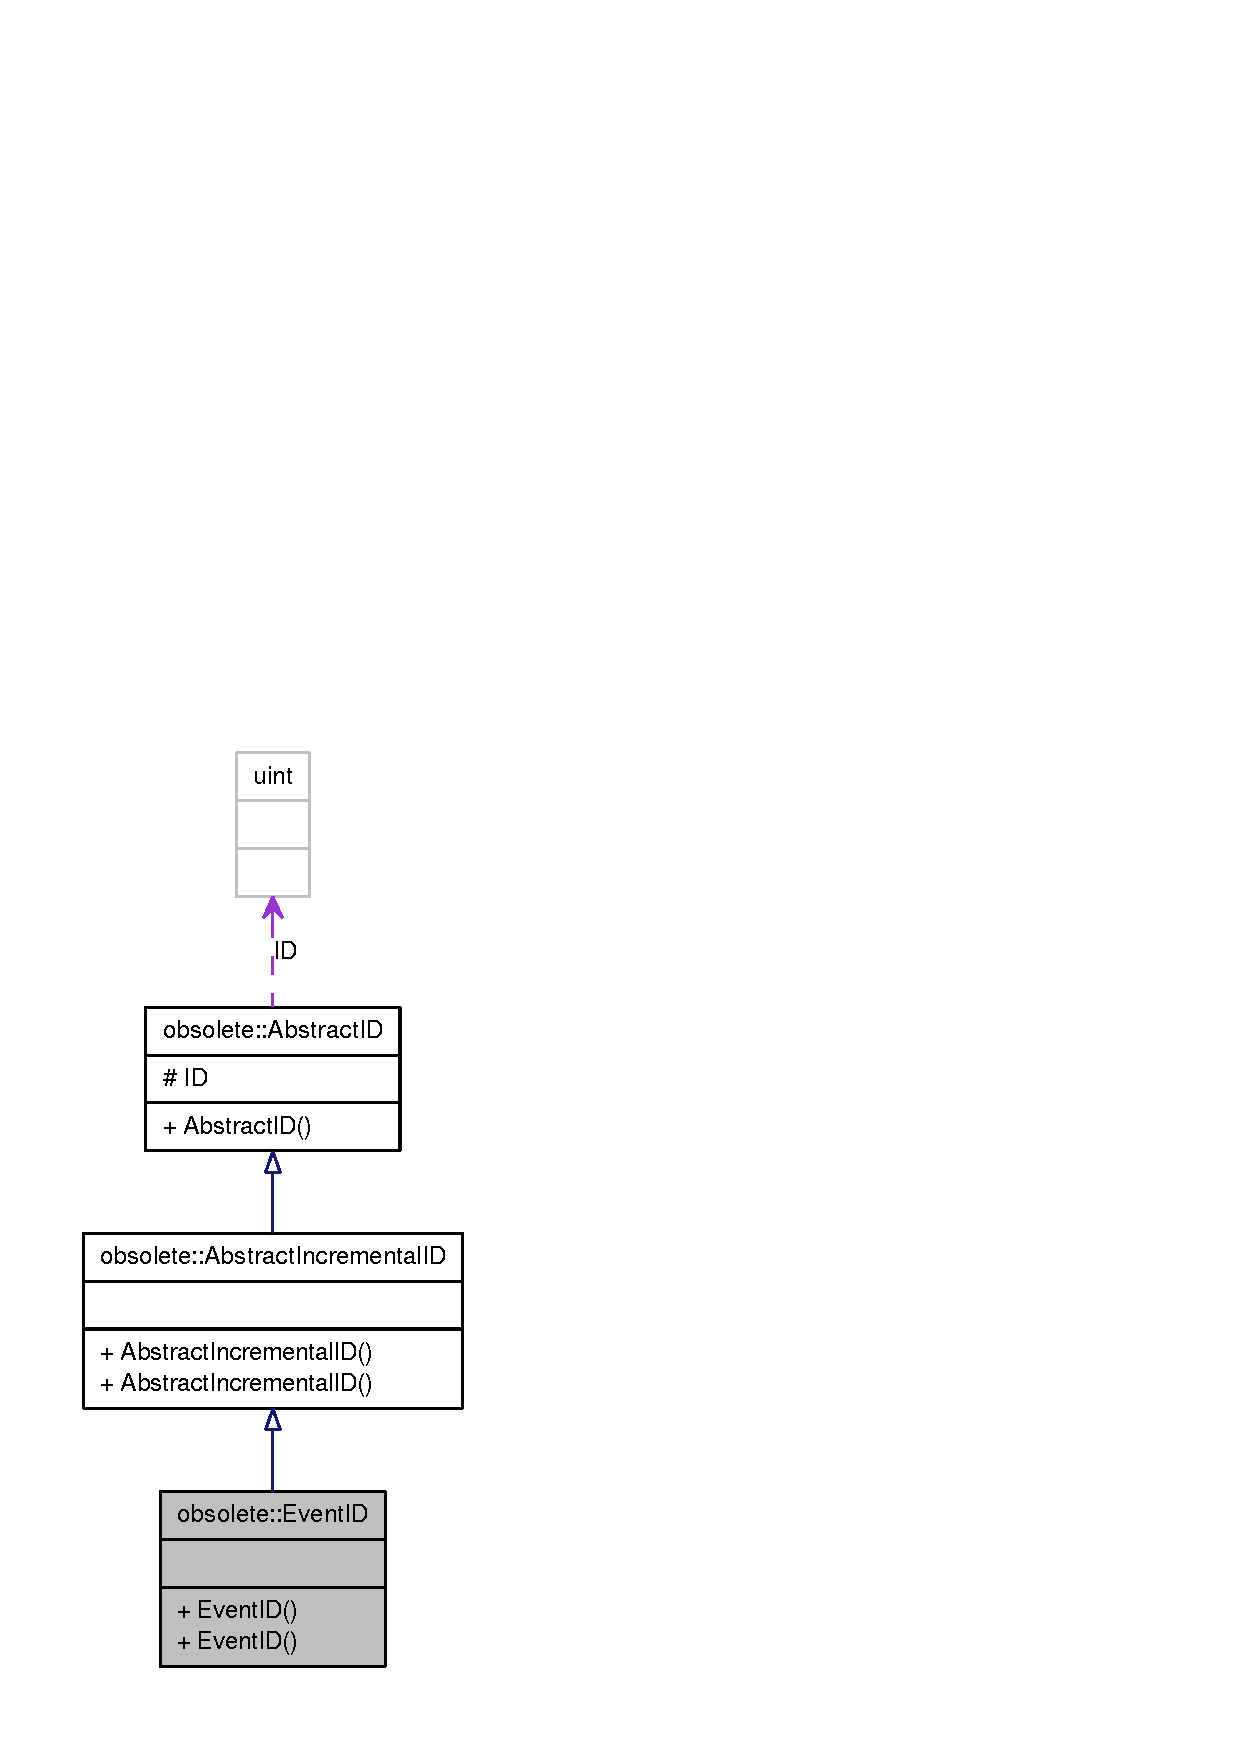
\includegraphics[height=400pt]{classobsolete_1_1EventID__coll__graph}
\end{center}
\end{figure}
\subsection*{Metody publiczne}
\begin{DoxyCompactItemize}
\item 
\hyperlink{classobsolete_1_1EventID_a56f3f261f5a5a15b298795fe2663e15d}{EventID} (uint \hyperlink{classobsolete_1_1ID}{ID})
\begin{DoxyCompactList}\small\item\em Wykorzystuje konstruktor klasy nadrzędnej. \item\end{DoxyCompactList}\item 
\hyperlink{classobsolete_1_1EventID_a6de0f2cb209f8a8fe5ebe42a1bb3644d}{EventID} ()
\begin{DoxyCompactList}\small\item\em Pozwalam również na tworzenie niezainicjalizowanych obiektów. \item\end{DoxyCompactList}\end{DoxyCompactItemize}
\subsection*{Atrybuty chronione}
\begin{DoxyCompactItemize}
\item 
uint \hyperlink{classobsolete_1_1AbstractID_a5f67fa1c7d96085f0ef41193b60b570c}{ID}
\begin{DoxyCompactList}\small\item\em Reprezentowany \hyperlink{classobsolete_1_1ID}{ID}. \item\end{DoxyCompactList}\end{DoxyCompactItemize}


\subsection{Opis szczegółowy}
Klasa reprezentująca identyfikator zdarzenia. 

Definicja w linii 10 pliku eventid.h.



\subsection{Dokumentacja konstruktora i destruktora}
\hypertarget{classobsolete_1_1EventID_a56f3f261f5a5a15b298795fe2663e15d}{
\index{obsolete::EventID@{obsolete::EventID}!EventID@{EventID}}
\index{EventID@{EventID}!obsolete::EventID@{obsolete::EventID}}
\subsubsection[{EventID}]{\setlength{\rightskip}{0pt plus 5cm}obsolete::EventID::EventID (uint {\em ID})\hspace{0.3cm}{\ttfamily  \mbox{[}inline\mbox{]}}}}
\label{classobsolete_1_1EventID_a56f3f261f5a5a15b298795fe2663e15d}


Wykorzystuje konstruktor klasy nadrzędnej. 



Definicja w linii 13 pliku eventid.h.

\hypertarget{classobsolete_1_1EventID_a6de0f2cb209f8a8fe5ebe42a1bb3644d}{
\index{obsolete::EventID@{obsolete::EventID}!EventID@{EventID}}
\index{EventID@{EventID}!obsolete::EventID@{obsolete::EventID}}
\subsubsection[{EventID}]{\setlength{\rightskip}{0pt plus 5cm}obsolete::EventID::EventID ()\hspace{0.3cm}{\ttfamily  \mbox{[}inline\mbox{]}}}}
\label{classobsolete_1_1EventID_a6de0f2cb209f8a8fe5ebe42a1bb3644d}


Pozwalam również na tworzenie niezainicjalizowanych obiektów. 



Definicja w linii 14 pliku eventid.h.



\subsection{Dokumentacja atrybutów składowych}
\hypertarget{classobsolete_1_1AbstractID_a5f67fa1c7d96085f0ef41193b60b570c}{
\index{obsolete::EventID@{obsolete::EventID}!ID@{ID}}
\index{ID@{ID}!obsolete::EventID@{obsolete::EventID}}
\subsubsection[{ID}]{\setlength{\rightskip}{0pt plus 5cm}uint {\bf obsolete::AbstractID::ID}\hspace{0.3cm}{\ttfamily  \mbox{[}protected, inherited\mbox{]}}}}
\label{classobsolete_1_1AbstractID_a5f67fa1c7d96085f0ef41193b60b570c}


Reprezentowany \hyperlink{classobsolete_1_1ID}{ID}. 



Definicja w linii 34 pliku abstractid.h.



Dokumentacja dla tej klasy została wygenerowana z pliku:\begin{DoxyCompactItemize}
\item 
include/obsolete/\hyperlink{eventid_8h}{eventid.h}\end{DoxyCompactItemize}

\hypertarget{classobsolete_1_1EventIDGenerator}{
\section{Dokumentacja klasy obsolete::EventIDGenerator}
\label{classobsolete_1_1EventIDGenerator}\index{obsolete::EventIDGenerator@{obsolete::EventIDGenerator}}
}


Klasa generatorów generatorów identyfikatorów wydarzeń.  




{\ttfamily \#include $<$eventidgenerator.h$>$}



Diagram dziedziczenia dla obsolete::EventIDGenerator\nopagebreak
\begin{figure}[H]
\begin{center}
\leavevmode
\includegraphics[width=218pt]{classobsolete_1_1EventIDGenerator__inherit__graph}
\end{center}
\end{figure}


Diagram współpracy dla obsolete::EventIDGenerator:\nopagebreak
\begin{figure}[H]
\begin{center}
\leavevmode
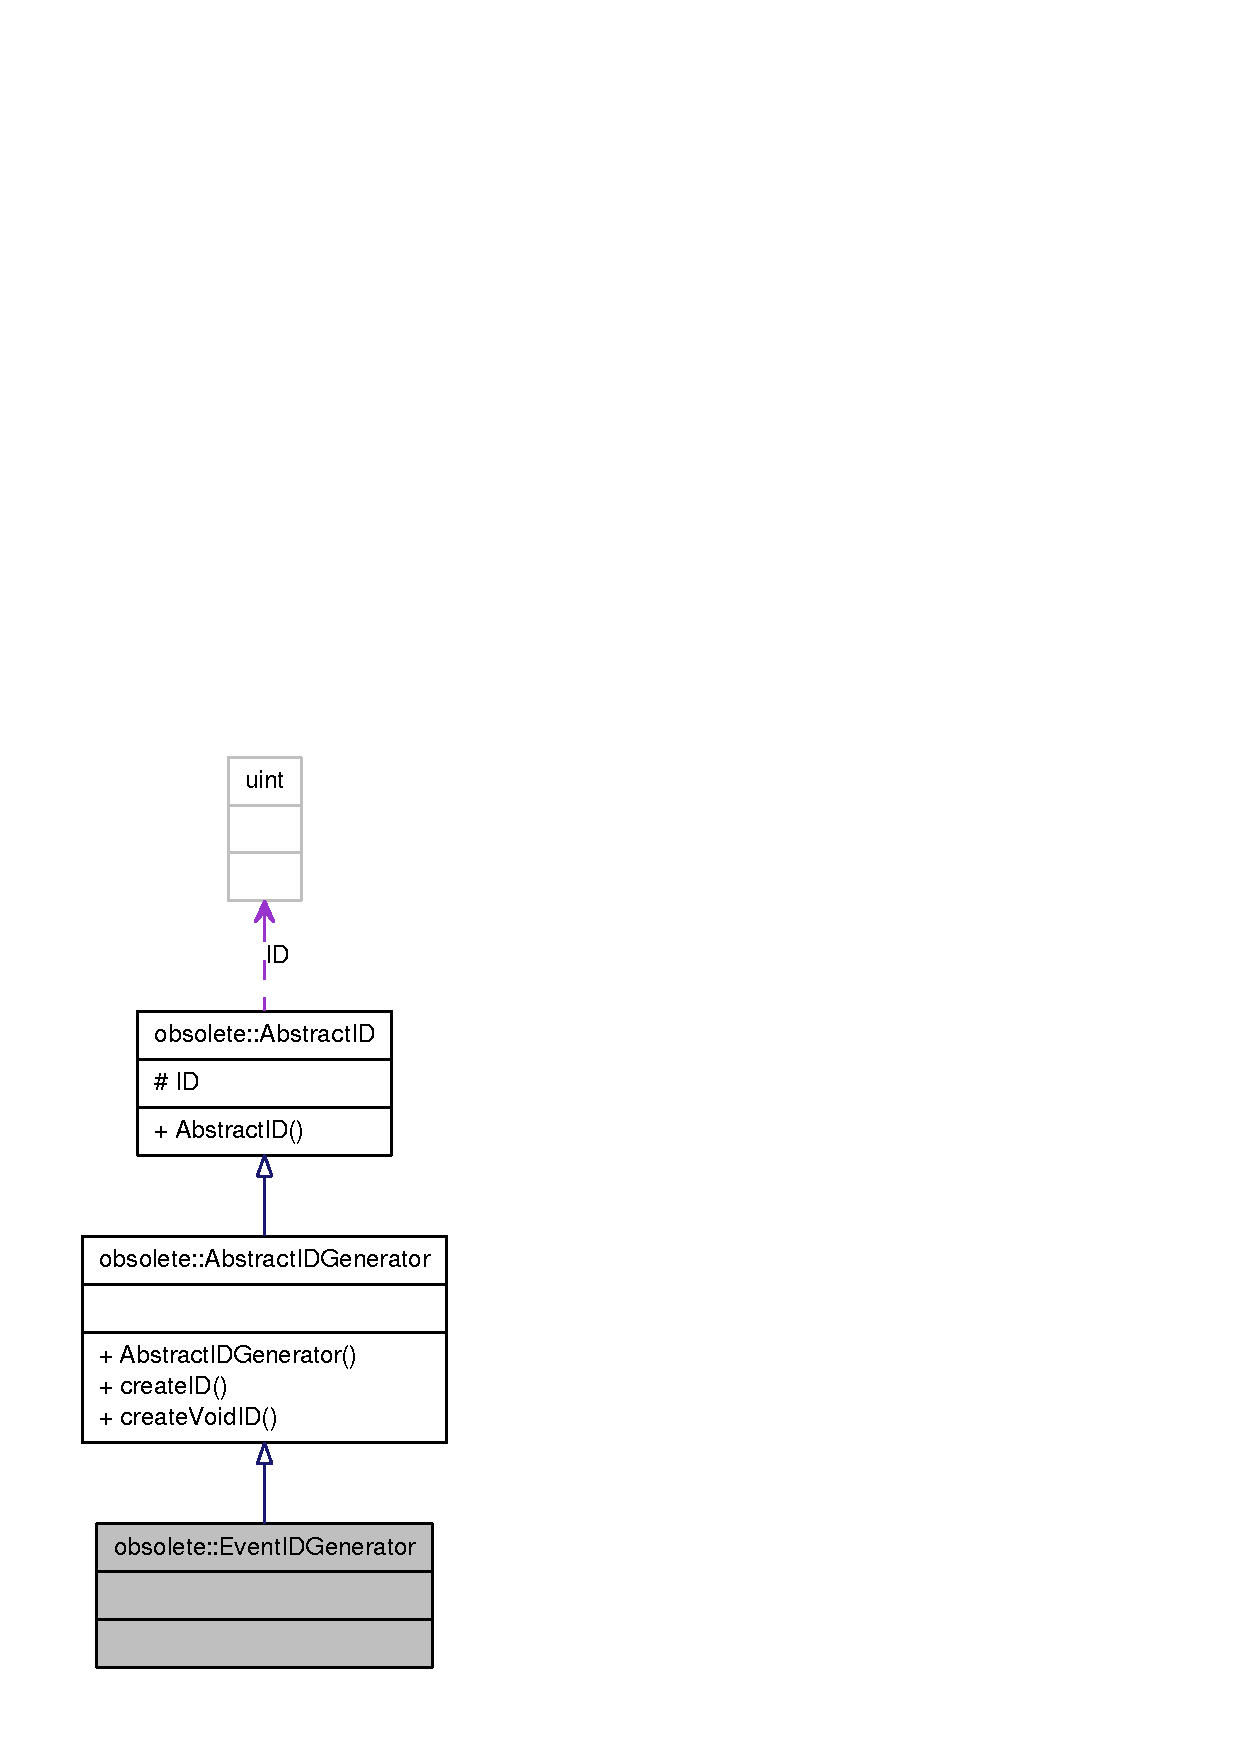
\includegraphics[height=400pt]{classobsolete_1_1EventIDGenerator__coll__graph}
\end{center}
\end{figure}
\subsection*{Metody publiczne}
\begin{DoxyCompactItemize}
\item 
virtual \hyperlink{classobsolete_1_1ID}{ID} \hyperlink{classobsolete_1_1AbstractIDGenerator_a39d2f0147e3a028fef8299770e23db90}{createID} ()
\begin{DoxyCompactList}\small\item\em Tworzy nowy identyfikator. \item\end{DoxyCompactList}\end{DoxyCompactItemize}
\subsection*{Statyczne metody publiczne}
\begin{DoxyCompactItemize}
\item 
static \hyperlink{classobsolete_1_1ID}{ID} \hyperlink{classobsolete_1_1AbstractIDGenerator_a330da88ba80820ca6ce0a29cbbab9e1b}{createVoidID} ()
\begin{DoxyCompactList}\small\item\em Tworzy niezainicjowany identyfikator. \item\end{DoxyCompactList}\end{DoxyCompactItemize}
\subsection*{Atrybuty chronione}
\begin{DoxyCompactItemize}
\item 
uint \hyperlink{classobsolete_1_1AbstractID_a5f67fa1c7d96085f0ef41193b60b570c}{ID}
\begin{DoxyCompactList}\small\item\em Reprezentowany \hyperlink{classobsolete_1_1ID}{ID}. \item\end{DoxyCompactList}\end{DoxyCompactItemize}


\subsection{Opis szczegółowy}
Klasa generatorów generatorów identyfikatorów wydarzeń. 

Definicja w linii 8 pliku eventidgenerator.h.



\subsection{Dokumentacja funkcji składowych}
\hypertarget{classobsolete_1_1AbstractIDGenerator_a39d2f0147e3a028fef8299770e23db90}{
\index{obsolete::EventIDGenerator@{obsolete::EventIDGenerator}!createID@{createID}}
\index{createID@{createID}!obsolete::EventIDGenerator@{obsolete::EventIDGenerator}}
\subsubsection[{createID}]{\setlength{\rightskip}{0pt plus 5cm}virtual {\bf ID} obsolete::AbstractIDGenerator::createID ()\hspace{0.3cm}{\ttfamily  \mbox{[}virtual, inherited\mbox{]}}}}
\label{classobsolete_1_1AbstractIDGenerator_a39d2f0147e3a028fef8299770e23db90}


Tworzy nowy identyfikator. 

\hypertarget{classobsolete_1_1AbstractIDGenerator_a330da88ba80820ca6ce0a29cbbab9e1b}{
\index{obsolete::EventIDGenerator@{obsolete::EventIDGenerator}!createVoidID@{createVoidID}}
\index{createVoidID@{createVoidID}!obsolete::EventIDGenerator@{obsolete::EventIDGenerator}}
\subsubsection[{createVoidID}]{\setlength{\rightskip}{0pt plus 5cm}static {\bf ID} obsolete::AbstractIDGenerator::createVoidID ()\hspace{0.3cm}{\ttfamily  \mbox{[}static, inherited\mbox{]}}}}
\label{classobsolete_1_1AbstractIDGenerator_a330da88ba80820ca6ce0a29cbbab9e1b}


Tworzy niezainicjowany identyfikator. 



\subsection{Dokumentacja atrybutów składowych}
\hypertarget{classobsolete_1_1AbstractID_a5f67fa1c7d96085f0ef41193b60b570c}{
\index{obsolete::EventIDGenerator@{obsolete::EventIDGenerator}!ID@{ID}}
\index{ID@{ID}!obsolete::EventIDGenerator@{obsolete::EventIDGenerator}}
\subsubsection[{ID}]{\setlength{\rightskip}{0pt plus 5cm}uint {\bf obsolete::AbstractID::ID}\hspace{0.3cm}{\ttfamily  \mbox{[}protected, inherited\mbox{]}}}}
\label{classobsolete_1_1AbstractID_a5f67fa1c7d96085f0ef41193b60b570c}


Reprezentowany \hyperlink{classobsolete_1_1ID}{ID}. 



Definicja w linii 34 pliku abstractid.h.



Dokumentacja dla tej klasy została wygenerowana z pliku:\begin{DoxyCompactItemize}
\item 
include/obsolete/\hyperlink{eventidgenerator_8h}{eventidgenerator.h}\end{DoxyCompactItemize}

\hypertarget{classEvents}{
\section{Dokumentacja klasy Events}
\label{classEvents}\index{Events@{Events}}
}


Klasa przechowuje wszystkie wydarzenia i zarządza nimi.  




{\ttfamily \#include $<$events.h$>$}



Diagram współpracy dla Events:\nopagebreak
\begin{figure}[H]
\begin{center}
\leavevmode
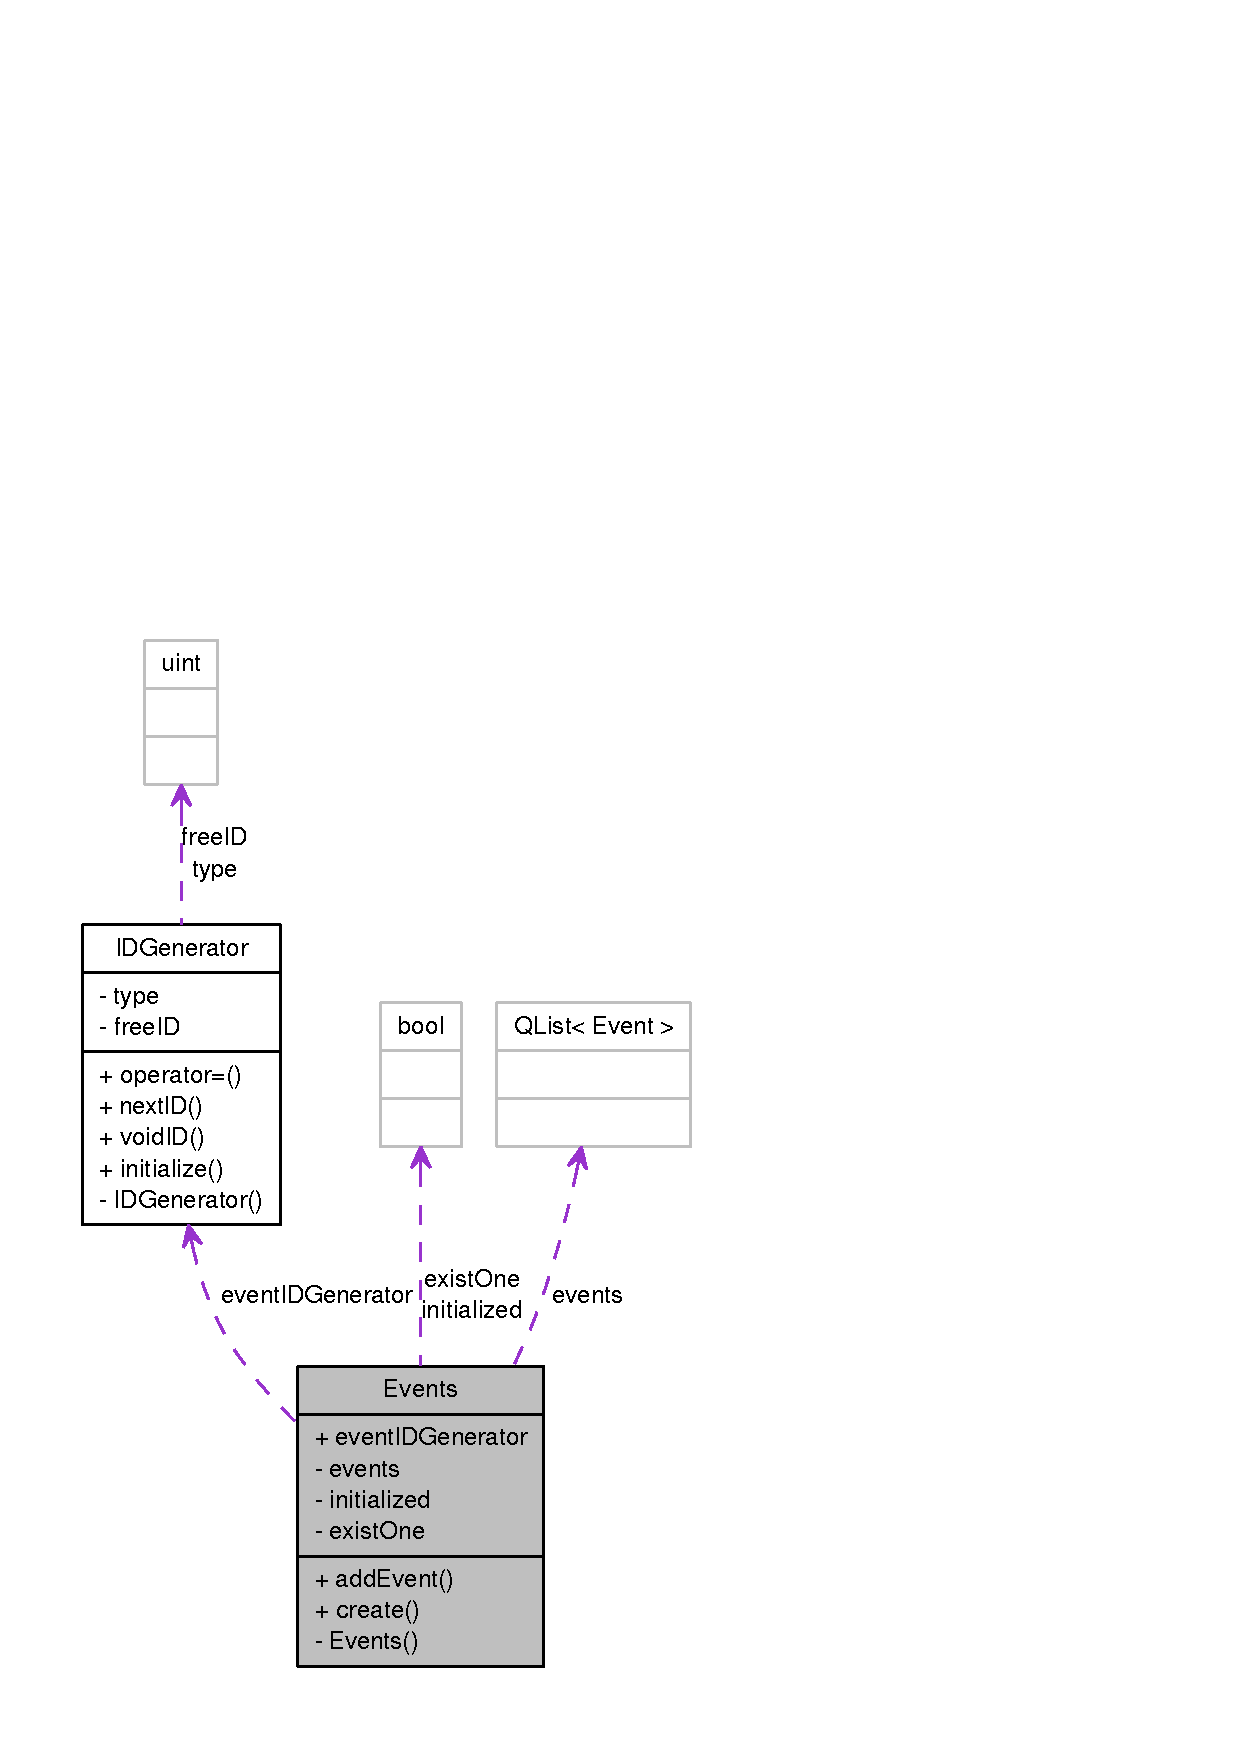
\includegraphics[height=400pt]{classEvents__coll__graph}
\end{center}
\end{figure}
\subsection*{Metody publiczne}
\begin{DoxyCompactItemize}
\item 
void \hyperlink{classEvents_afb346fb0339e89dd2093dec8f0620da7}{addEvent} (\hyperlink{classEvent}{Event} newEvent)
\begin{DoxyCompactList}\small\item\em Dodaje nowe wydarzenie. \item\end{DoxyCompactList}\end{DoxyCompactItemize}
\subsection*{Statyczne metody publiczne}
\begin{DoxyCompactItemize}
\item 
static \hyperlink{classEvents}{Events} \hyperlink{classEvents_ac4ccb0fd05c7bc876b95cf6cdd549666}{create} ()  throw (char$\ast$)
\begin{DoxyCompactList}\small\item\em Tworzy instancje klasy. \item\end{DoxyCompactList}\end{DoxyCompactItemize}
\subsection*{Atrybuty publiczne}
\begin{DoxyCompactItemize}
\item 
\hyperlink{classIDGenerator}{IDGenerator} \hyperlink{classEvents_aee8768258412e3f8d298a539e038169c}{eventIDGenerator}
\begin{DoxyCompactList}\small\item\em Generator identyfikatorów wydarzeń. \item\end{DoxyCompactList}\end{DoxyCompactItemize}
\subsection*{Metody prywatne}
\begin{DoxyCompactItemize}
\item 
\hyperlink{classEvents_aab651428bab6b09db3564753afb225a6}{Events} ()
\begin{DoxyCompactList}\small\item\em Oznacza nowy obiekt jako niezainicjalizowany. \item\end{DoxyCompactList}\end{DoxyCompactItemize}
\subsection*{Atrybuty prywatne}
\begin{DoxyCompactItemize}
\item 
QList$<$ \hyperlink{classEvent}{Event} $>$ \hyperlink{classEvents_a38bc398f90e69e671e7411bf73cf3fc0}{events}
\begin{DoxyCompactList}\small\item\em Lista wszystkich wydarzeń. Będzie się powiększać. \item\end{DoxyCompactList}\item 
bool \hyperlink{classEvents_a155926e71d11323e83ceb574177b01cb}{initialized}
\begin{DoxyCompactList}\small\item\em Czy obiekt tej klasy został zainicjalizowany. \item\end{DoxyCompactList}\end{DoxyCompactItemize}
\subsection*{Statyczne atrybuty prywatne}
\begin{DoxyCompactItemize}
\item 
static bool \hyperlink{classEvents_a5b2f7b7d038ce9447080499b0736c4fe}{existOne}
\begin{DoxyCompactList}\small\item\em Czy istnieje jakiś obiekt tej klasy. \item\end{DoxyCompactList}\end{DoxyCompactItemize}
\subsection*{Przyjaciele}
\begin{DoxyCompactItemize}
\item 
QDataStream \& \hyperlink{classEvents_a560f3fdc9b76a9fe9146335122ecda39}{operator$<$$<$} (QDataStream \&stream, const \hyperlink{classEvents}{Events} \&\hyperlink{classEvents_a38bc398f90e69e671e7411bf73cf3fc0}{events})
\begin{DoxyCompactList}\small\item\em Zapisuje informacje o wydarzeniach do danego strumienia. \item\end{DoxyCompactList}\item 
QDataStream \& \hyperlink{classEvents_a9e3a2b909c5dcbc9519365ccafc4a96f}{operator$>$$>$} (QDataStream \&stream, \hyperlink{classEvents}{Events} \&\hyperlink{classEvents_a38bc398f90e69e671e7411bf73cf3fc0}{events})
\begin{DoxyCompactList}\small\item\em Odczytuje informacje o wydarzeniach z danego strumienia. \item\end{DoxyCompactList}\end{DoxyCompactItemize}


\subsection{Opis szczegółowy}
Klasa przechowuje wszystkie wydarzenia i zarządza nimi. 

Definicja w linii 11 pliku events.h.



\subsection{Dokumentacja konstruktora i destruktora}
\hypertarget{classEvents_aab651428bab6b09db3564753afb225a6}{
\index{Events@{Events}!Events@{Events}}
\index{Events@{Events}!Events@{Events}}
\subsubsection[{Events}]{\setlength{\rightskip}{0pt plus 5cm}Events::Events ()\hspace{0.3cm}{\ttfamily  \mbox{[}inline, private\mbox{]}}}}
\label{classEvents_aab651428bab6b09db3564753afb225a6}


Oznacza nowy obiekt jako niezainicjalizowany. 



Definicja w linii 47 pliku events.h.



Odwołania w create().




\begin{DoxyCode}
50 :
\end{DoxyCode}




Oto graf wywoływań tej funkcji:\nopagebreak
\begin{figure}[H]
\begin{center}
\leavevmode
\includegraphics[width=133pt]{classEvents_aab651428bab6b09db3564753afb225a6_icgraph}
\end{center}
\end{figure}




\subsection{Dokumentacja funkcji składowych}
\hypertarget{classEvents_afb346fb0339e89dd2093dec8f0620da7}{
\index{Events@{Events}!addEvent@{addEvent}}
\index{addEvent@{addEvent}!Events@{Events}}
\subsubsection[{addEvent}]{\setlength{\rightskip}{0pt plus 5cm}void Events::addEvent ({\bf Event} {\em newEvent})}}
\label{classEvents_afb346fb0339e89dd2093dec8f0620da7}


Dodaje nowe wydarzenie. 


\begin{DoxyParams}{Parametry}
\item[{\em newEvent}]Wydarzenie które ma zostać dodane do bazy danych. \end{DoxyParams}


Definicja w linii 15 pliku events.cpp.



Odwołuje się do events.




\begin{DoxyCode}
16 {
17     Events::events<<newEvent;
18 }
\end{DoxyCode}


\hypertarget{classEvents_ac4ccb0fd05c7bc876b95cf6cdd549666}{
\index{Events@{Events}!create@{create}}
\index{create@{create}!Events@{Events}}
\subsubsection[{create}]{\setlength{\rightskip}{0pt plus 5cm}{\bf Events} Events::create ()  throw (char$\ast$)\hspace{0.3cm}{\ttfamily  \mbox{[}static\mbox{]}}}}
\label{classEvents_ac4ccb0fd05c7bc876b95cf6cdd549666}


Tworzy instancje klasy. 


\begin{DoxyExceptions}{Wyjątki}
\item[{\em char$\ast$}]Jeżeli już wywołano tę metodę \end{DoxyExceptions}
\begin{DoxyReturn}{Zwraca}
Nowy obiekt tej klasy 
\end{DoxyReturn}


Definicja w linii 20 pliku events.cpp.



Odwołuje się do Events() i existOne.




\begin{DoxyCode}
21 {
22     if (existOne)
23         throw "Obiekt już istnieje!";
24     existOne=true;
25     return Events();
26 }
\end{DoxyCode}




Oto graf wywołań dla tej funkcji:\nopagebreak
\begin{figure}[H]
\begin{center}
\leavevmode
\includegraphics[width=133pt]{classEvents_ac4ccb0fd05c7bc876b95cf6cdd549666_cgraph}
\end{center}
\end{figure}




\subsection{Dokumentacja przyjaciół i funkcji związanych}
\hypertarget{classEvents_a560f3fdc9b76a9fe9146335122ecda39}{
\index{Events@{Events}!operator$<$$<$@{operator$<$$<$}}
\index{operator$<$$<$@{operator$<$$<$}!Events@{Events}}
\subsubsection[{operator$<$$<$}]{\setlength{\rightskip}{0pt plus 5cm}QDataStream\& operator$<$$<$ (QDataStream \& {\em stream}, \/  const {\bf Events} \& {\em events})\hspace{0.3cm}{\ttfamily  \mbox{[}friend\mbox{]}}}}
\label{classEvents_a560f3fdc9b76a9fe9146335122ecda39}


Zapisuje informacje o wydarzeniach do danego strumienia. 


\begin{DoxyParams}{Parametry}
\item[{\em stream}]Strumień do którego będą zapisywane dane. \item[{\em events}]Wydarzenia które będzie zapisywane. \end{DoxyParams}
\begin{DoxyReturn}{Zwraca}
Ten sam strumień. 
\end{DoxyReturn}


Definicja w linii 5 pliku events.cpp.




\begin{DoxyCode}
6 {
7     return stream<<events.eventIDGenerator<<events.events;
8 }
\end{DoxyCode}


\hypertarget{classEvents_a9e3a2b909c5dcbc9519365ccafc4a96f}{
\index{Events@{Events}!operator$>$$>$@{operator$>$$>$}}
\index{operator$>$$>$@{operator$>$$>$}!Events@{Events}}
\subsubsection[{operator$>$$>$}]{\setlength{\rightskip}{0pt plus 5cm}QDataStream\& operator$>$$>$ (QDataStream \& {\em stream}, \/  {\bf Events} \& {\em events})\hspace{0.3cm}{\ttfamily  \mbox{[}friend\mbox{]}}}}
\label{classEvents_a9e3a2b909c5dcbc9519365ccafc4a96f}


Odczytuje informacje o wydarzeniach z danego strumienia. 


\begin{DoxyParams}{Parametry}
\item[{\em stream}]Strumień z którego będą odczytywane dane. \item[{\em events}]Obiekt klasy \hyperlink{classEvents}{Events} który zostanie zainicjalizowany wczytanymi danymi. \end{DoxyParams}
\begin{DoxyReturn}{Zwraca}
Ten sam strumień. 
\end{DoxyReturn}


Definicja w linii 10 pliku events.cpp.




\begin{DoxyCode}
11 {
12     return stream>>events.eventIDGenerator>>events.events;
13 }
\end{DoxyCode}




\subsection{Dokumentacja atrybutów składowych}
\hypertarget{classEvents_aee8768258412e3f8d298a539e038169c}{
\index{Events@{Events}!eventIDGenerator@{eventIDGenerator}}
\index{eventIDGenerator@{eventIDGenerator}!Events@{Events}}
\subsubsection[{eventIDGenerator}]{\setlength{\rightskip}{0pt plus 5cm}{\bf IDGenerator} {\bf Events::eventIDGenerator}}}
\label{classEvents_aee8768258412e3f8d298a539e038169c}


Generator identyfikatorów wydarzeń. 



Definicja w linii 24 pliku events.h.



Odwołania w operator$<$$<$() i operator$>$$>$().

\hypertarget{classEvents_a38bc398f90e69e671e7411bf73cf3fc0}{
\index{Events@{Events}!events@{events}}
\index{events@{events}!Events@{Events}}
\subsubsection[{events}]{\setlength{\rightskip}{0pt plus 5cm}QList$<${\bf Event}$>$ {\bf Events::events}\hspace{0.3cm}{\ttfamily  \mbox{[}private\mbox{]}}}}
\label{classEvents_a38bc398f90e69e671e7411bf73cf3fc0}


Lista wszystkich wydarzeń. Będzie się powiększać. 



Definicja w linii 26 pliku events.h.



Odwołania w addEvent(), operator$<$$<$() i operator$>$$>$().

\hypertarget{classEvents_a5b2f7b7d038ce9447080499b0736c4fe}{
\index{Events@{Events}!existOne@{existOne}}
\index{existOne@{existOne}!Events@{Events}}
\subsubsection[{existOne}]{\setlength{\rightskip}{0pt plus 5cm}bool {\bf Events::existOne}\hspace{0.3cm}{\ttfamily  \mbox{[}static, private\mbox{]}}}}
\label{classEvents_a5b2f7b7d038ce9447080499b0736c4fe}


Czy istnieje jakiś obiekt tej klasy. 



Definicja w linii 29 pliku events.h.



Odwołania w create().

\hypertarget{classEvents_a155926e71d11323e83ceb574177b01cb}{
\index{Events@{Events}!initialized@{initialized}}
\index{initialized@{initialized}!Events@{Events}}
\subsubsection[{initialized}]{\setlength{\rightskip}{0pt plus 5cm}bool {\bf Events::initialized}\hspace{0.3cm}{\ttfamily  \mbox{[}private\mbox{]}}}}
\label{classEvents_a155926e71d11323e83ceb574177b01cb}


Czy obiekt tej klasy został zainicjalizowany. 



Definicja w linii 28 pliku events.h.



Dokumentacja dla tej klasy została wygenerowana z plików:\begin{DoxyCompactItemize}
\item 
include/\hyperlink{events_8h}{events.h}\item 
src/\hyperlink{events_8cpp}{events.cpp}\end{DoxyCompactItemize}

\hypertarget{classGeneratorIDGenerator}{
\section{Dokumentacja klasy GeneratorIDGenerator}
\label{classGeneratorIDGenerator}\index{GeneratorIDGenerator@{GeneratorIDGenerator}}
}


Ta klasa odpowiada za generowanie generatorów identyfikatorów.  




{\ttfamily \#include $<$generatoridgenerator.h$>$}



Diagram współpracy dla GeneratorIDGenerator:\nopagebreak
\begin{figure}[H]
\begin{center}
\leavevmode
\includegraphics[width=202pt]{classGeneratorIDGenerator__coll__graph}
\end{center}
\end{figure}
\subsection*{Statyczne metody publiczne}
\begin{DoxyCompactItemize}
\item 
static \hyperlink{classIDGenerator}{IDGenerator} \hyperlink{classGeneratorIDGenerator_ac6dd43ecbbe2ed1647855e72156dbcb2}{nextIDGenerator} ()
\begin{DoxyCompactList}\small\item\em Generuje następny generator identyfikatorów. \item\end{DoxyCompactList}\item 
static \hyperlink{classIDGenerator}{IDGenerator} \hyperlink{classGeneratorIDGenerator_af0d8b94b08eac9bfbeea41ef974d8745}{voidIDGenerator} ()
\begin{DoxyCompactList}\small\item\em Generuje niezainicjalizowany (błędny) generator identyfikatorów. \item\end{DoxyCompactList}\end{DoxyCompactItemize}
\subsection*{Metody prywatne}
\begin{DoxyCompactItemize}
\item 
\hyperlink{classGeneratorIDGenerator_a659b541be9156e0ad96561c7f2a4cbd6}{GeneratorIDGenerator} ()
\begin{DoxyCompactList}\small\item\em Nie pozwalam na tworzenie obiektów tej klasy. \item\end{DoxyCompactList}\end{DoxyCompactItemize}
\subsection*{Statyczne atrybuty prywatne}
\begin{DoxyCompactItemize}
\item 
static uint \hyperlink{classGeneratorIDGenerator_a6df8dcb43ce1c7e5f2d4610dfaf1d19e}{freeIDGenerator} = 1
\begin{DoxyCompactList}\small\item\em Pierwszy dostępny typ Generatora identyfikatorów. \item\end{DoxyCompactList}\end{DoxyCompactItemize}


\subsection{Opis szczegółowy}
Ta klasa odpowiada za generowanie generatorów identyfikatorów. 

Definicja w linii 7 pliku generatoridgenerator.h.



\subsection{Dokumentacja konstruktora i destruktora}
\hypertarget{classGeneratorIDGenerator_a659b541be9156e0ad96561c7f2a4cbd6}{
\index{GeneratorIDGenerator@{GeneratorIDGenerator}!GeneratorIDGenerator@{GeneratorIDGenerator}}
\index{GeneratorIDGenerator@{GeneratorIDGenerator}!GeneratorIDGenerator@{GeneratorIDGenerator}}
\subsubsection[{GeneratorIDGenerator}]{\setlength{\rightskip}{0pt plus 5cm}GeneratorIDGenerator::GeneratorIDGenerator ()\hspace{0.3cm}{\ttfamily  \mbox{[}inline, private\mbox{]}}}}
\label{classGeneratorIDGenerator_a659b541be9156e0ad96561c7f2a4cbd6}


Nie pozwalam na tworzenie obiektów tej klasy. 



Definicja w linii 20 pliku generatoridgenerator.h.




\begin{DoxyCode}
20 {}
\end{DoxyCode}




\subsection{Dokumentacja funkcji składowych}
\hypertarget{classGeneratorIDGenerator_ac6dd43ecbbe2ed1647855e72156dbcb2}{
\index{GeneratorIDGenerator@{GeneratorIDGenerator}!nextIDGenerator@{nextIDGenerator}}
\index{nextIDGenerator@{nextIDGenerator}!GeneratorIDGenerator@{GeneratorIDGenerator}}
\subsubsection[{nextIDGenerator}]{\setlength{\rightskip}{0pt plus 5cm}{\bf IDGenerator} GeneratorIDGenerator::nextIDGenerator ()\hspace{0.3cm}{\ttfamily  \mbox{[}static\mbox{]}}}}
\label{classGeneratorIDGenerator_ac6dd43ecbbe2ed1647855e72156dbcb2}


Generuje następny generator identyfikatorów. 



Definicja w linii 5 pliku generatoridgenerator.cpp.



Odwołuje się do freeIDGenerator.



Odwołania w IDGenerator::initialize() i main().




\begin{DoxyCode}
6 {
7     return IDGenerator(freeIDGenerator++);
8 }
\end{DoxyCode}




Oto graf wywoływań tej funkcji:\nopagebreak
\begin{figure}[H]
\begin{center}
\leavevmode
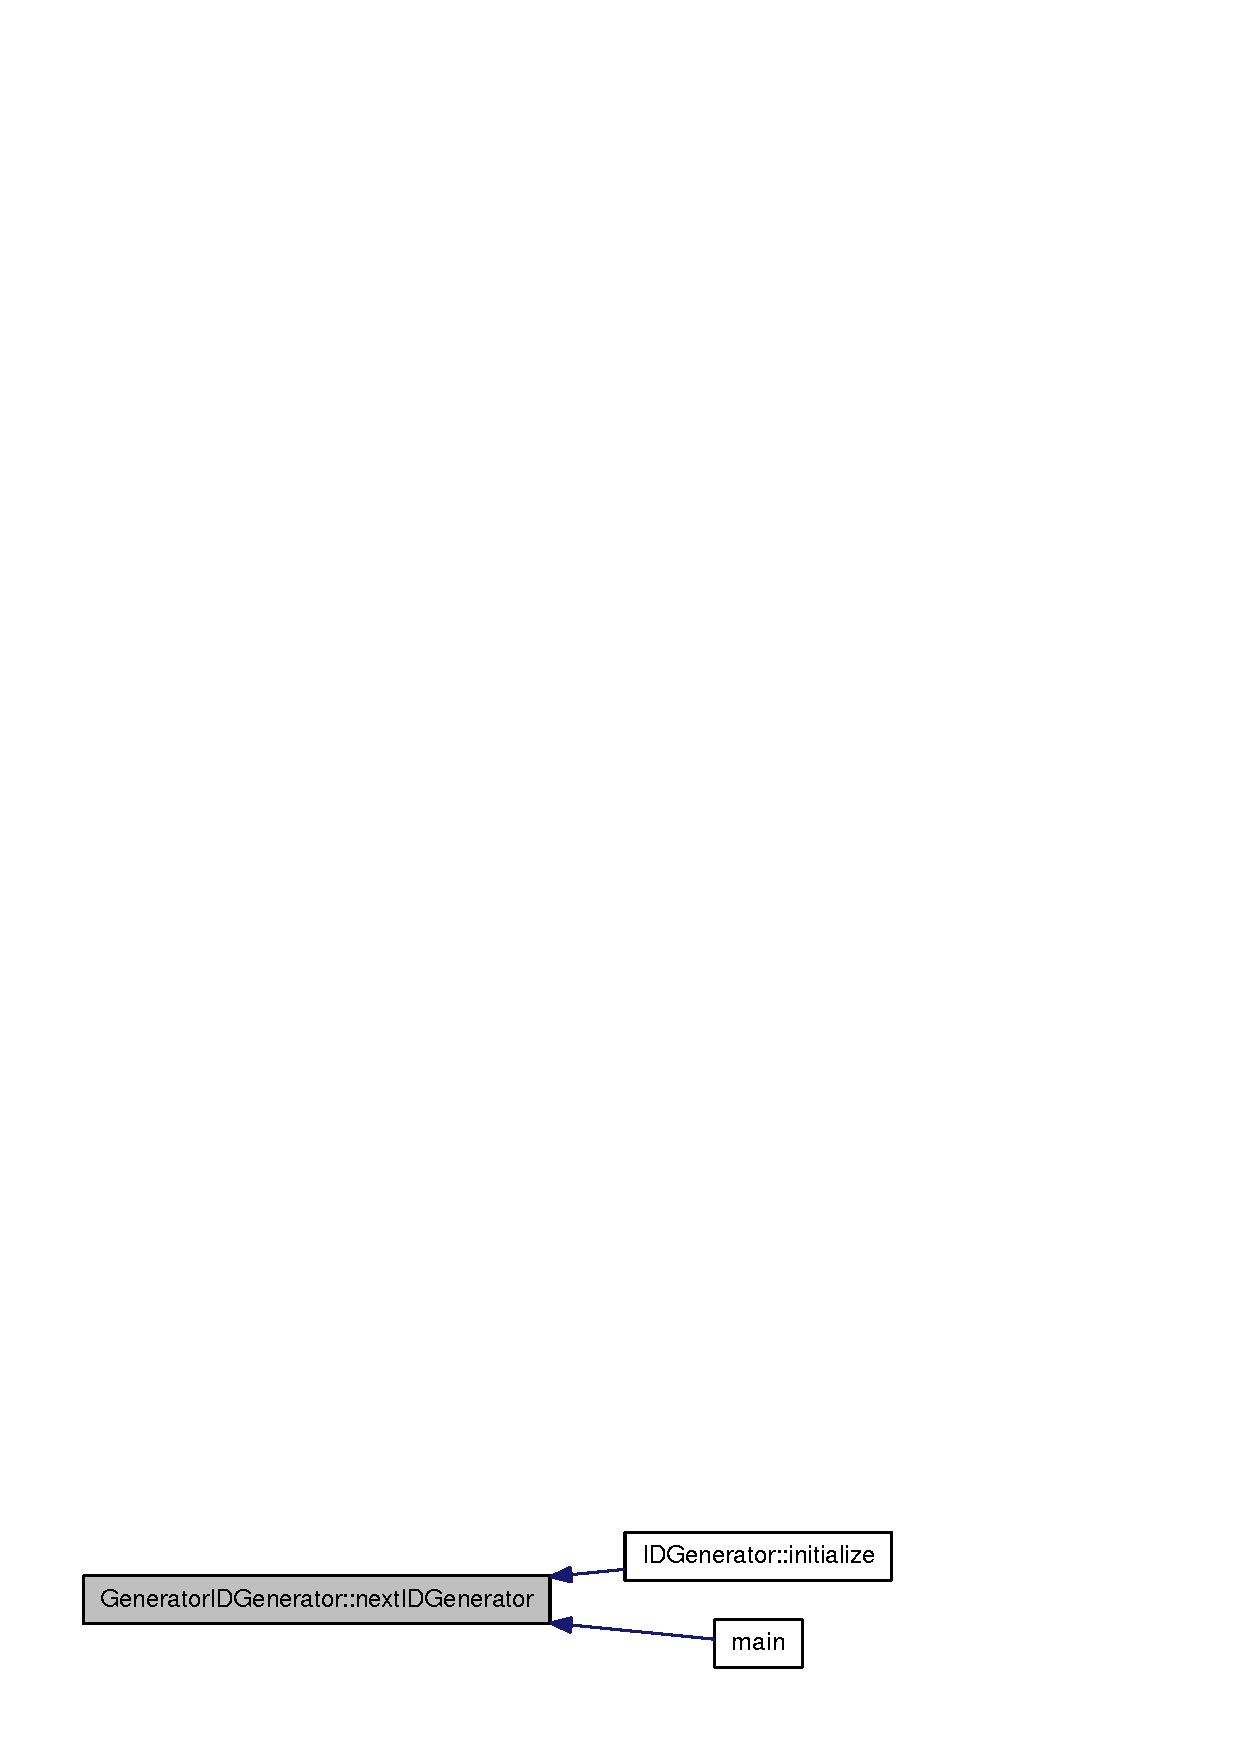
\includegraphics[width=216pt]{classGeneratorIDGenerator_ac6dd43ecbbe2ed1647855e72156dbcb2_icgraph}
\end{center}
\end{figure}


\hypertarget{classGeneratorIDGenerator_af0d8b94b08eac9bfbeea41ef974d8745}{
\index{GeneratorIDGenerator@{GeneratorIDGenerator}!voidIDGenerator@{voidIDGenerator}}
\index{voidIDGenerator@{voidIDGenerator}!GeneratorIDGenerator@{GeneratorIDGenerator}}
\subsubsection[{voidIDGenerator}]{\setlength{\rightskip}{0pt plus 5cm}{\bf IDGenerator} GeneratorIDGenerator::voidIDGenerator ()\hspace{0.3cm}{\ttfamily  \mbox{[}static\mbox{]}}}}
\label{classGeneratorIDGenerator_af0d8b94b08eac9bfbeea41ef974d8745}


Generuje niezainicjalizowany (błędny) generator identyfikatorów. 



Definicja w linii 10 pliku generatoridgenerator.cpp.




\begin{DoxyCode}
11 {
12     return IDGenerator(0);
13 }
\end{DoxyCode}




\subsection{Dokumentacja atrybutów składowych}
\hypertarget{classGeneratorIDGenerator_a6df8dcb43ce1c7e5f2d4610dfaf1d19e}{
\index{GeneratorIDGenerator@{GeneratorIDGenerator}!freeIDGenerator@{freeIDGenerator}}
\index{freeIDGenerator@{freeIDGenerator}!GeneratorIDGenerator@{GeneratorIDGenerator}}
\subsubsection[{freeIDGenerator}]{\setlength{\rightskip}{0pt plus 5cm}uint {\bf GeneratorIDGenerator::freeIDGenerator} = 1\hspace{0.3cm}{\ttfamily  \mbox{[}static, private\mbox{]}}}}
\label{classGeneratorIDGenerator_a6df8dcb43ce1c7e5f2d4610dfaf1d19e}


Pierwszy dostępny typ Generatora identyfikatorów. 



Definicja w linii 11 pliku generatoridgenerator.h.



Odwołania w nextIDGenerator().



Dokumentacja dla tej klasy została wygenerowana z plików:\begin{DoxyCompactItemize}
\item 
include/\hyperlink{generatoridgenerator_8h}{generatoridgenerator.h}\item 
src/\hyperlink{generatoridgenerator_8cpp}{generatoridgenerator.cpp}\end{DoxyCompactItemize}

\hypertarget{classIDGenerator_1_1ID}{
\section{Dokumentacja klasy IDGenerator::ID}
\label{classIDGenerator_1_1ID}\index{IDGenerator::ID@{IDGenerator::ID}}
}


Obiekt reprezentuje dany identyfikator określonego typu.  




{\ttfamily \#include $<$idgenerator.h$>$}



Diagram współpracy dla IDGenerator::ID:\nopagebreak
\begin{figure}[H]
\begin{center}
\leavevmode
\includegraphics[width=142pt]{classIDGenerator_1_1ID__coll__graph}
\end{center}
\end{figure}
\subsection*{Metody publiczne}
\begin{DoxyCompactItemize}
\item 
\hyperlink{classIDGenerator_1_1ID_aadc91850d9ea6ba775aa07b7f214a7a5}{ID} ()
\begin{DoxyCompactList}\small\item\em Konstruktor domyślny. \item\end{DoxyCompactList}\item 
\hyperlink{classIDGenerator_1_1ID}{ID} \& \hyperlink{classIDGenerator_1_1ID_a239f6a12bb0b8ddf74bc5a8e2fdffdf4}{operator=} (const \hyperlink{classIDGenerator_1_1ID}{ID} \&o)  throw (char$\ast$)
\begin{DoxyCompactList}\small\item\em Przypisuje wartość identyfikatora do pustego identyfikatora. \item\end{DoxyCompactList}\end{DoxyCompactItemize}
\subsection*{Metody prywatne}
\begin{DoxyCompactItemize}
\item 
\hyperlink{classIDGenerator_1_1ID_af7801ab8a1caefa26b551274e5e0530b}{ID} (uint \hyperlink{classIDGenerator_1_1ID_a284b4a6d5b96b758a3ba11b5539d0878}{id}, uint \hyperlink{classIDGenerator_1_1ID_a336d735ce48e2bca744bc7d77c6792af}{type})
\begin{DoxyCompactList}\small\item\em Inicjalizuje identyfikator. \item\end{DoxyCompactList}\end{DoxyCompactItemize}
\subsection*{Atrybuty prywatne}
\begin{DoxyCompactItemize}
\item 
uint \hyperlink{classIDGenerator_1_1ID_a284b4a6d5b96b758a3ba11b5539d0878}{id}
\begin{DoxyCompactList}\small\item\em Reprezentowany \hyperlink{classIDGenerator_1_1ID}{ID}. \item\end{DoxyCompactList}\item 
uint \hyperlink{classIDGenerator_1_1ID_a336d735ce48e2bca744bc7d77c6792af}{type}
\begin{DoxyCompactList}\small\item\em Typ tego identyfikatora. \item\end{DoxyCompactList}\end{DoxyCompactItemize}
\subsection*{Przyjaciele}
\begin{DoxyCompactItemize}
\item 
class \hyperlink{classIDGenerator_1_1ID_a85bc66475d72826ee03d9f388d7fcd0f}{IDGenerator}
\begin{DoxyCompactList}\small\item\em Identyfikator jest zaprzyjaźniony ze swoim stwórcą. \item\end{DoxyCompactList}\item 
QDataStream \& \hyperlink{classIDGenerator_1_1ID_ac7c84abfa059c0c94c7a0c53ffe2b4fc}{operator$<$$<$} (QDataStream \&stream, const \hyperlink{classIDGenerator_1_1ID}{ID} \&\hyperlink{classIDGenerator_1_1ID_a284b4a6d5b96b758a3ba11b5539d0878}{id})
\begin{DoxyCompactList}\small\item\em Zapisuje dany identyfikator do danego strumienia. \item\end{DoxyCompactList}\item 
QDataStream \& \hyperlink{classIDGenerator_1_1ID_a30f4c9e493a25817666bb64ce4fd1168}{operator$>$$>$} (QDataStream \&stream, \hyperlink{classIDGenerator_1_1ID}{ID} \&\hyperlink{classIDGenerator_1_1ID_a284b4a6d5b96b758a3ba11b5539d0878}{id})
\begin{DoxyCompactList}\small\item\em Odczytuje dany identyfikator z danego strumienia. \item\end{DoxyCompactList}\end{DoxyCompactItemize}


\subsection{Opis szczegółowy}
Obiekt reprezentuje dany identyfikator określonego typu. 

Definicja w linii 29 pliku idgenerator.h.



\subsection{Dokumentacja konstruktora i destruktora}
\hypertarget{classIDGenerator_1_1ID_aadc91850d9ea6ba775aa07b7f214a7a5}{
\index{IDGenerator::ID@{IDGenerator::ID}!ID@{ID}}
\index{ID@{ID}!IDGenerator::ID@{IDGenerator::ID}}
\subsubsection[{ID}]{\setlength{\rightskip}{0pt plus 5cm}IDGenerator::ID::ID ()\hspace{0.3cm}{\ttfamily  \mbox{[}inline\mbox{]}}}}
\label{classIDGenerator_1_1ID_aadc91850d9ea6ba775aa07b7f214a7a5}


Konstruktor domyślny. 



Definicja w linii 54 pliku idgenerator.h.




\begin{DoxyCode}
54 : id(0),type(0) {}
\end{DoxyCode}


\hypertarget{classIDGenerator_1_1ID_af7801ab8a1caefa26b551274e5e0530b}{
\index{IDGenerator::ID@{IDGenerator::ID}!ID@{ID}}
\index{ID@{ID}!IDGenerator::ID@{IDGenerator::ID}}
\subsubsection[{ID}]{\setlength{\rightskip}{0pt plus 5cm}IDGenerator::ID::ID (uint {\em id}, \/  uint {\em type})\hspace{0.3cm}{\ttfamily  \mbox{[}inline, private\mbox{]}}}}
\label{classIDGenerator_1_1ID_af7801ab8a1caefa26b551274e5e0530b}


Inicjalizuje identyfikator. 



Definicja w linii 61 pliku idgenerator.h.




\begin{DoxyCode}
61 : id(id), type(type) {}
\end{DoxyCode}




\subsection{Dokumentacja funkcji składowych}
\hypertarget{classIDGenerator_1_1ID_a239f6a12bb0b8ddf74bc5a8e2fdffdf4}{
\index{IDGenerator::ID@{IDGenerator::ID}!operator=@{operator=}}
\index{operator=@{operator=}!IDGenerator::ID@{IDGenerator::ID}}
\subsubsection[{operator=}]{\setlength{\rightskip}{0pt plus 5cm}{\bf IDGenerator::ID} \& IDGenerator::ID::operator= (const {\bf ID} \& {\em o})  throw (char$\ast$)}}
\label{classIDGenerator_1_1ID_a239f6a12bb0b8ddf74bc5a8e2fdffdf4}


Przypisuje wartość identyfikatora do pustego identyfikatora. 



Definicja w linii 40 pliku idgenerator.cpp.



Odwołuje się do id.




\begin{DoxyCode}
41 {
42     if (type!=0 || (type==o.type && o.id==0))
43         throw "Nie wolno nadpisywać identyfikatorów!";
44     id=o.id;
45     type=o.type;
46     return *this;
47 }
\end{DoxyCode}




\subsection{Dokumentacja przyjaciół i funkcji związanych}
\hypertarget{classIDGenerator_1_1ID_a85bc66475d72826ee03d9f388d7fcd0f}{
\index{IDGenerator::ID@{IDGenerator::ID}!IDGenerator@{IDGenerator}}
\index{IDGenerator@{IDGenerator}!IDGenerator::ID@{IDGenerator::ID}}
\subsubsection[{IDGenerator}]{\setlength{\rightskip}{0pt plus 5cm}friend class {\bf IDGenerator}\hspace{0.3cm}{\ttfamily  \mbox{[}friend\mbox{]}}}}
\label{classIDGenerator_1_1ID_a85bc66475d72826ee03d9f388d7fcd0f}


Identyfikator jest zaprzyjaźniony ze swoim stwórcą. 



Definicja w linii 32 pliku idgenerator.h.

\hypertarget{classIDGenerator_1_1ID_ac7c84abfa059c0c94c7a0c53ffe2b4fc}{
\index{IDGenerator::ID@{IDGenerator::ID}!operator$<$$<$@{operator$<$$<$}}
\index{operator$<$$<$@{operator$<$$<$}!IDGenerator::ID@{IDGenerator::ID}}
\subsubsection[{operator$<$$<$}]{\setlength{\rightskip}{0pt plus 5cm}QDataStream\& operator$<$$<$ (QDataStream \& {\em stream}, \/  const {\bf ID} \& {\em id})\hspace{0.3cm}{\ttfamily  \mbox{[}friend\mbox{]}}}}
\label{classIDGenerator_1_1ID_ac7c84abfa059c0c94c7a0c53ffe2b4fc}


Zapisuje dany identyfikator do danego strumienia. 


\begin{DoxyParams}{Parametry}
\item[{\em stream}]Strumień do którego będzie zapisany identyfikator. \item[{\em id}]Identyfikator który zostanie zapisany. \end{DoxyParams}
\begin{DoxyReturn}{Zwraca}
Ten sam strumień. 
\end{DoxyReturn}


Definicja w linii 20 pliku idgenerator.cpp.




\begin{DoxyCode}
21 {
22     return stream<<id.type<<id.id;
23 }
\end{DoxyCode}


\hypertarget{classIDGenerator_1_1ID_a30f4c9e493a25817666bb64ce4fd1168}{
\index{IDGenerator::ID@{IDGenerator::ID}!operator$>$$>$@{operator$>$$>$}}
\index{operator$>$$>$@{operator$>$$>$}!IDGenerator::ID@{IDGenerator::ID}}
\subsubsection[{operator$>$$>$}]{\setlength{\rightskip}{0pt plus 5cm}QDataStream\& operator$>$$>$ (QDataStream \& {\em stream}, \/  {\bf IDGenerator::ID} \& {\em id})\hspace{0.3cm}{\ttfamily  \mbox{[}friend\mbox{]}}}}
\label{classIDGenerator_1_1ID_a30f4c9e493a25817666bb64ce4fd1168}


Odczytuje dany identyfikator z danego strumienia. 


\begin{DoxyParams}{Parametry}
\item[{\em stream}]Strumień z którego będzie odczytany identyfikator. \item[{\em id}]Identyfikator który zostanie zainicjalizowany odczytanymi danymi. \end{DoxyParams}
\begin{DoxyReturn}{Zwraca}
Ten sam strumień. 
\end{DoxyReturn}


Definicja w linii 25 pliku idgenerator.cpp.




\begin{DoxyCode}
26 {
27     return stream>>id.type>>id.id;
28 }
\end{DoxyCode}




\subsection{Dokumentacja atrybutów składowych}
\hypertarget{classIDGenerator_1_1ID_a284b4a6d5b96b758a3ba11b5539d0878}{
\index{IDGenerator::ID@{IDGenerator::ID}!id@{id}}
\index{id@{id}!IDGenerator::ID@{IDGenerator::ID}}
\subsubsection[{id}]{\setlength{\rightskip}{0pt plus 5cm}uint {\bf IDGenerator::ID::id}\hspace{0.3cm}{\ttfamily  \mbox{[}private\mbox{]}}}}
\label{classIDGenerator_1_1ID_a284b4a6d5b96b758a3ba11b5539d0878}


Reprezentowany \hyperlink{classIDGenerator_1_1ID}{ID}. 



Definicja w linii 50 pliku idgenerator.h.



Odwołania w operator=().

\hypertarget{classIDGenerator_1_1ID_a336d735ce48e2bca744bc7d77c6792af}{
\index{IDGenerator::ID@{IDGenerator::ID}!type@{type}}
\index{type@{type}!IDGenerator::ID@{IDGenerator::ID}}
\subsubsection[{type}]{\setlength{\rightskip}{0pt plus 5cm}uint {\bf IDGenerator::ID::type}\hspace{0.3cm}{\ttfamily  \mbox{[}private\mbox{]}}}}
\label{classIDGenerator_1_1ID_a336d735ce48e2bca744bc7d77c6792af}


Typ tego identyfikatora. 



Definicja w linii 51 pliku idgenerator.h.



Dokumentacja dla tej klasy została wygenerowana z plików:\begin{DoxyCompactItemize}
\item 
include/\hyperlink{idgenerator_8h}{idgenerator.h}\item 
src/\hyperlink{idgenerator_8cpp}{idgenerator.cpp}\end{DoxyCompactItemize}

\hypertarget{classobsolete_1_1ID}{
\section{Dokumentacja klasy obsolete::ID}
\label{classobsolete_1_1ID}\index{obsolete::ID@{obsolete::ID}}
}


Korzeń nowej idei uniwersalnego \hyperlink{classobsolete_1_1ID}{ID}.  




{\ttfamily \#include $<$id.h$>$}



Diagram dziedziczenia dla obsolete::ID\nopagebreak
\begin{figure}[H]
\begin{center}
\leavevmode
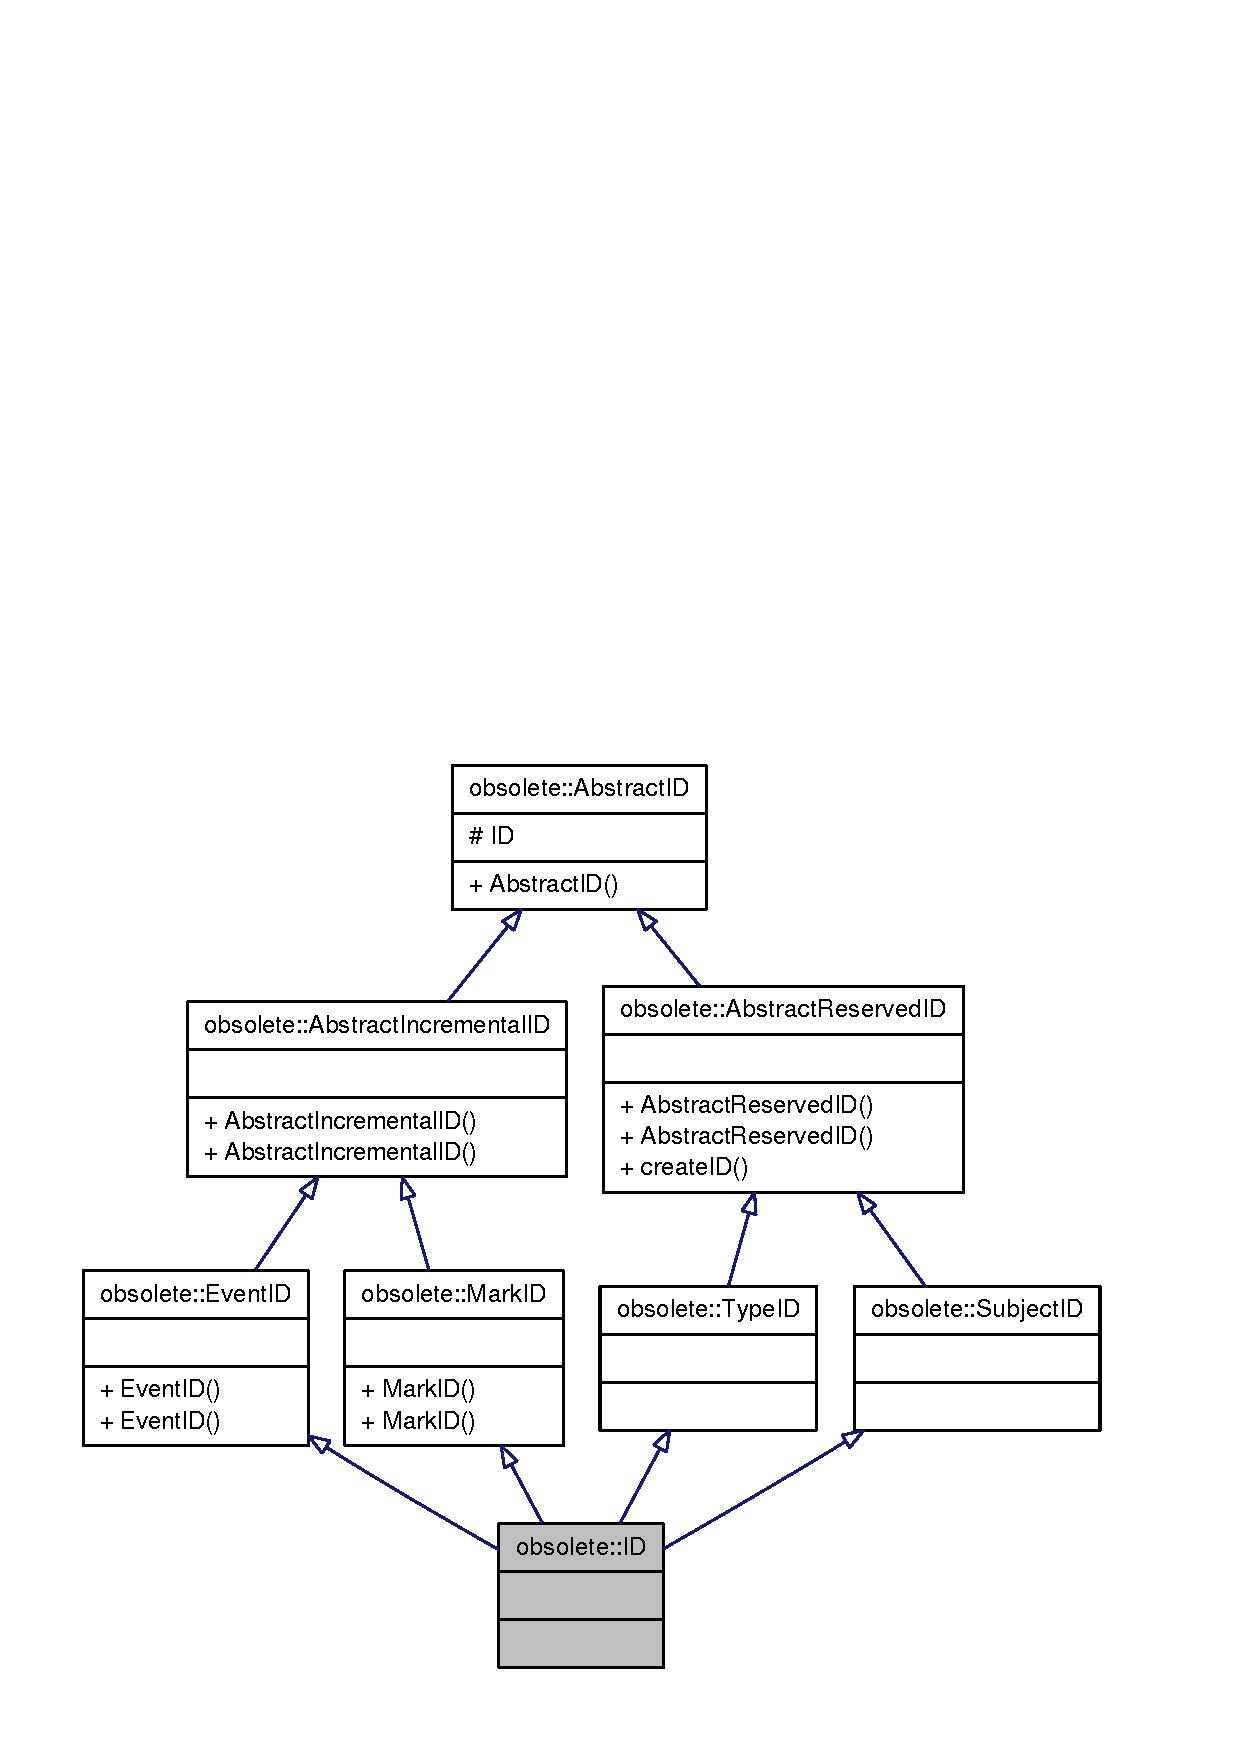
\includegraphics[width=400pt]{classobsolete_1_1ID__inherit__graph}
\end{center}
\end{figure}


Diagram współpracy dla obsolete::ID:\nopagebreak
\begin{figure}[H]
\begin{center}
\leavevmode
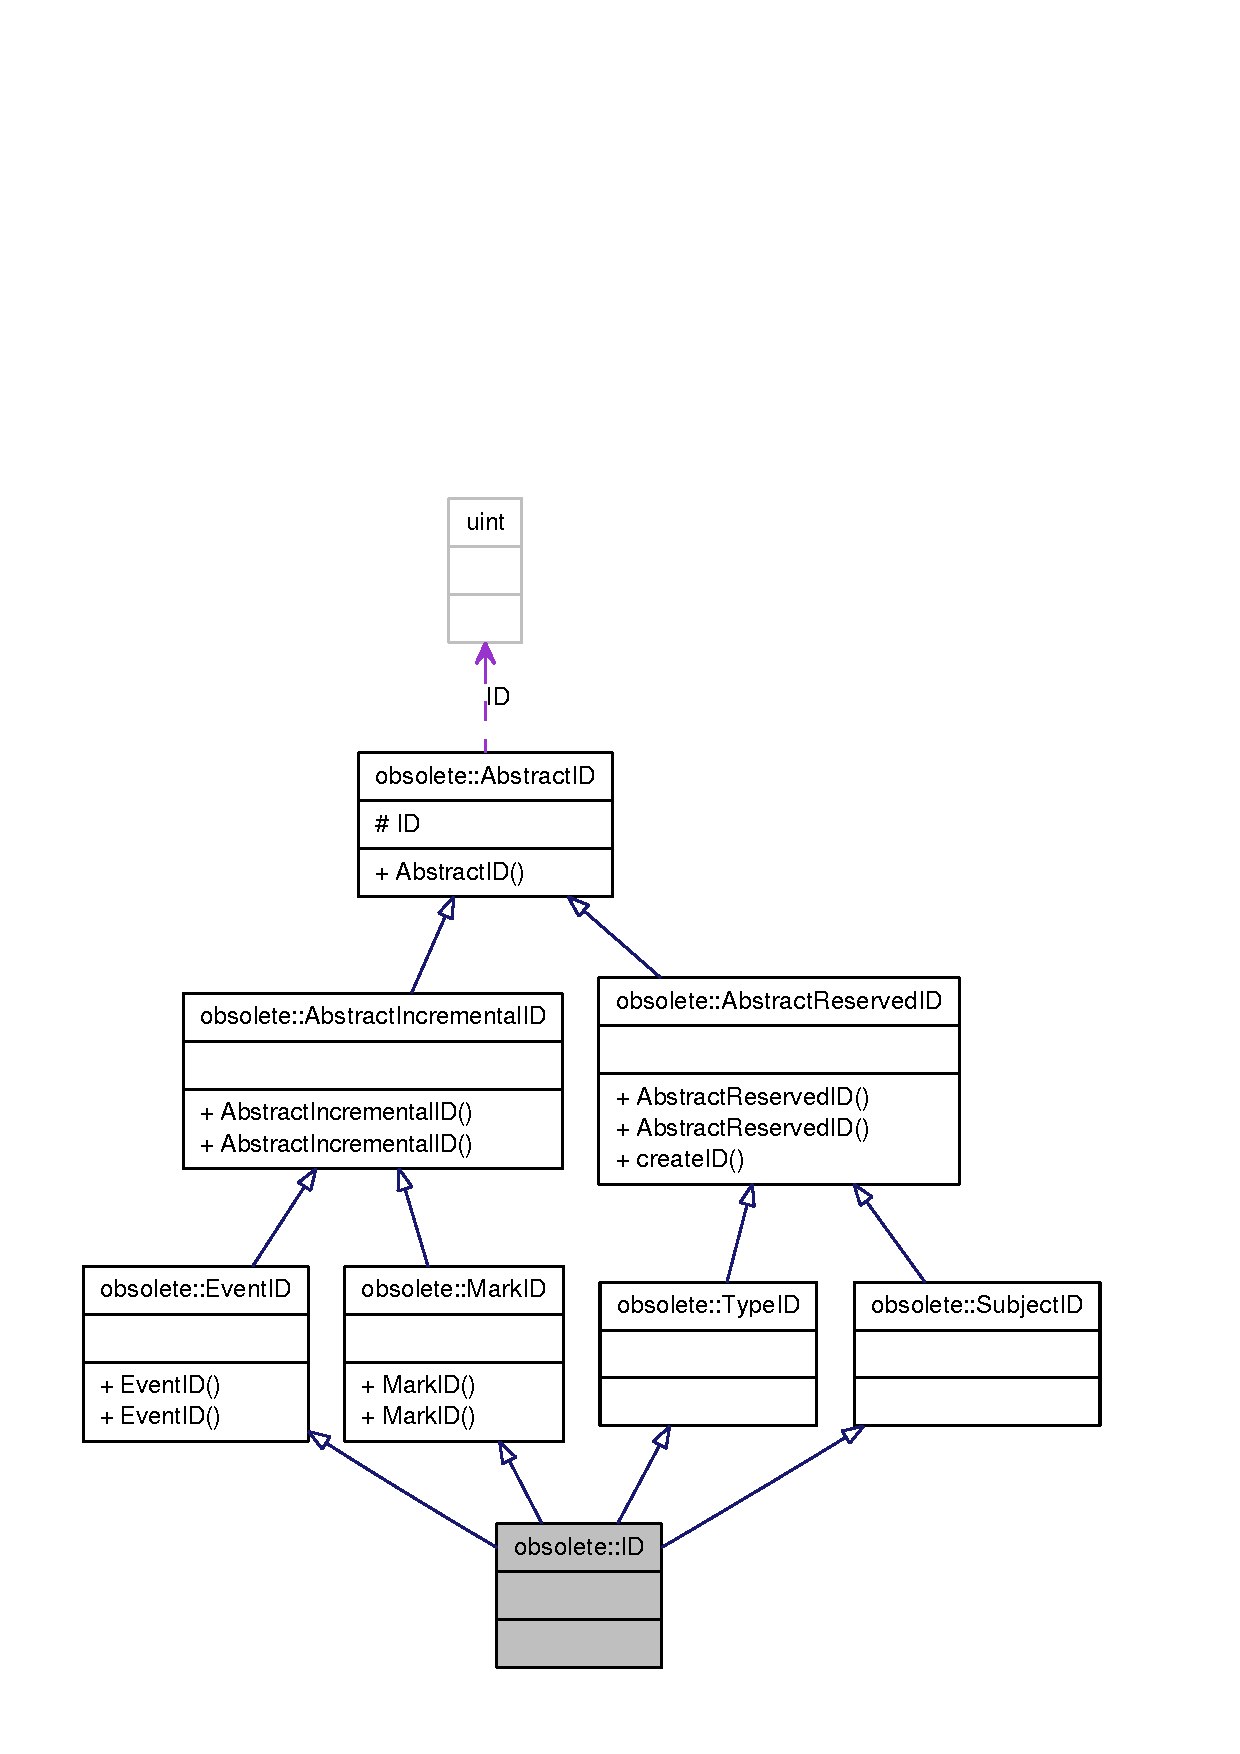
\includegraphics[width=400pt]{classobsolete_1_1ID__coll__graph}
\end{center}
\end{figure}
\subsection*{Statyczne metody publiczne}
\begin{DoxyCompactItemize}
\item 
static \hyperlink{classobsolete_1_1AbstractReservedID}{AbstractReservedID} \hyperlink{classobsolete_1_1AbstractReservedID_a38fa00bf6097ab9cff285c8480c8097e}{createID} (uint \hyperlink{classobsolete_1_1ID}{ID})
\begin{DoxyCompactList}\small\item\em Opakowuje numer porządkowy zadaną liczbą. \item\end{DoxyCompactList}\item 
static \hyperlink{classobsolete_1_1AbstractReservedID}{AbstractReservedID} \hyperlink{classobsolete_1_1AbstractReservedID_a38fa00bf6097ab9cff285c8480c8097e}{createID} (uint \hyperlink{classobsolete_1_1ID}{ID})
\begin{DoxyCompactList}\small\item\em Opakowuje numer porządkowy zadaną liczbą. \item\end{DoxyCompactList}\end{DoxyCompactItemize}
\subsection*{Atrybuty chronione}
\begin{DoxyCompactItemize}
\item 
uint \hyperlink{classobsolete_1_1AbstractID_a5f67fa1c7d96085f0ef41193b60b570c}{ID}
\begin{DoxyCompactList}\small\item\em Reprezentowany \hyperlink{classobsolete_1_1ID}{ID}. \item\end{DoxyCompactList}\item 
uint \hyperlink{classobsolete_1_1AbstractID_a5f67fa1c7d96085f0ef41193b60b570c}{ID}
\begin{DoxyCompactList}\small\item\em Reprezentowany \hyperlink{classobsolete_1_1ID}{ID}. \item\end{DoxyCompactList}\item 
uint \hyperlink{classobsolete_1_1AbstractID_a5f67fa1c7d96085f0ef41193b60b570c}{ID}
\begin{DoxyCompactList}\small\item\em Reprezentowany \hyperlink{classobsolete_1_1ID}{ID}. \item\end{DoxyCompactList}\item 
uint \hyperlink{classobsolete_1_1AbstractID_a5f67fa1c7d96085f0ef41193b60b570c}{ID}
\begin{DoxyCompactList}\small\item\em Reprezentowany \hyperlink{classobsolete_1_1ID}{ID}. \item\end{DoxyCompactList}\end{DoxyCompactItemize}


\subsection{Opis szczegółowy}
Korzeń nowej idei uniwersalnego \hyperlink{classobsolete_1_1ID}{ID}. 

Definicja w linii 13 pliku id.h.



\subsection{Dokumentacja funkcji składowych}
\hypertarget{classobsolete_1_1AbstractReservedID_a38fa00bf6097ab9cff285c8480c8097e}{
\index{obsolete::ID@{obsolete::ID}!createID@{createID}}
\index{createID@{createID}!obsolete::ID@{obsolete::ID}}
\subsubsection[{createID}]{\setlength{\rightskip}{0pt plus 5cm}static {\bf AbstractReservedID} obsolete::AbstractReservedID::createID (uint {\em ID})\hspace{0.3cm}{\ttfamily  \mbox{[}inline, static, inherited\mbox{]}}}}
\label{classobsolete_1_1AbstractReservedID_a38fa00bf6097ab9cff285c8480c8097e}


Opakowuje numer porządkowy zadaną liczbą. 

\hypertarget{classobsolete_1_1AbstractReservedID_a38fa00bf6097ab9cff285c8480c8097e}{
\index{obsolete::ID@{obsolete::ID}!createID@{createID}}
\index{createID@{createID}!obsolete::ID@{obsolete::ID}}
\subsubsection[{createID}]{\setlength{\rightskip}{0pt plus 5cm}static {\bf AbstractReservedID} obsolete::AbstractReservedID::createID (uint {\em ID})\hspace{0.3cm}{\ttfamily  \mbox{[}inline, static, inherited\mbox{]}}}}
\label{classobsolete_1_1AbstractReservedID_a38fa00bf6097ab9cff285c8480c8097e}


Opakowuje numer porządkowy zadaną liczbą. 



\subsection{Dokumentacja atrybutów składowych}
\hypertarget{classobsolete_1_1AbstractID_a5f67fa1c7d96085f0ef41193b60b570c}{
\index{obsolete::ID@{obsolete::ID}!ID@{ID}}
\index{ID@{ID}!obsolete::ID@{obsolete::ID}}
\subsubsection[{ID}]{\setlength{\rightskip}{0pt plus 5cm}uint {\bf obsolete::AbstractID::ID}\hspace{0.3cm}{\ttfamily  \mbox{[}protected, inherited\mbox{]}}}}
\label{classobsolete_1_1AbstractID_a5f67fa1c7d96085f0ef41193b60b570c}


Reprezentowany \hyperlink{classobsolete_1_1ID}{ID}. 



Definicja w linii 34 pliku abstractid.h.

\hypertarget{classobsolete_1_1AbstractID_a5f67fa1c7d96085f0ef41193b60b570c}{
\index{obsolete::ID@{obsolete::ID}!ID@{ID}}
\index{ID@{ID}!obsolete::ID@{obsolete::ID}}
\subsubsection[{ID}]{\setlength{\rightskip}{0pt plus 5cm}uint {\bf obsolete::AbstractID::ID}\hspace{0.3cm}{\ttfamily  \mbox{[}protected, inherited\mbox{]}}}}
\label{classobsolete_1_1AbstractID_a5f67fa1c7d96085f0ef41193b60b570c}


Reprezentowany \hyperlink{classobsolete_1_1ID}{ID}. 



Definicja w linii 34 pliku abstractid.h.

\hypertarget{classobsolete_1_1AbstractID_a5f67fa1c7d96085f0ef41193b60b570c}{
\index{obsolete::ID@{obsolete::ID}!ID@{ID}}
\index{ID@{ID}!obsolete::ID@{obsolete::ID}}
\subsubsection[{ID}]{\setlength{\rightskip}{0pt plus 5cm}uint {\bf obsolete::AbstractID::ID}\hspace{0.3cm}{\ttfamily  \mbox{[}protected, inherited\mbox{]}}}}
\label{classobsolete_1_1AbstractID_a5f67fa1c7d96085f0ef41193b60b570c}


Reprezentowany \hyperlink{classobsolete_1_1ID}{ID}. 



Definicja w linii 34 pliku abstractid.h.

\hypertarget{classobsolete_1_1AbstractID_a5f67fa1c7d96085f0ef41193b60b570c}{
\index{obsolete::ID@{obsolete::ID}!ID@{ID}}
\index{ID@{ID}!obsolete::ID@{obsolete::ID}}
\subsubsection[{ID}]{\setlength{\rightskip}{0pt plus 5cm}uint {\bf obsolete::AbstractID::ID}\hspace{0.3cm}{\ttfamily  \mbox{[}protected, inherited\mbox{]}}}}
\label{classobsolete_1_1AbstractID_a5f67fa1c7d96085f0ef41193b60b570c}


Reprezentowany \hyperlink{classobsolete_1_1ID}{ID}. 



Definicja w linii 34 pliku abstractid.h.



Dokumentacja dla tej klasy została wygenerowana z pliku:\begin{DoxyCompactItemize}
\item 
include/obsolete/\hyperlink{id_8h}{id.h}\end{DoxyCompactItemize}

\hypertarget{classIDGenerator}{
\section{Dokumentacja klasy IDGenerator}
\label{classIDGenerator}\index{IDGenerator@{IDGenerator}}
}


Generator identyfikatorów określonego typu.  




{\ttfamily \#include $<$idgenerator.h$>$}



Diagram współpracy dla IDGenerator:\nopagebreak
\begin{figure}[H]
\begin{center}
\leavevmode
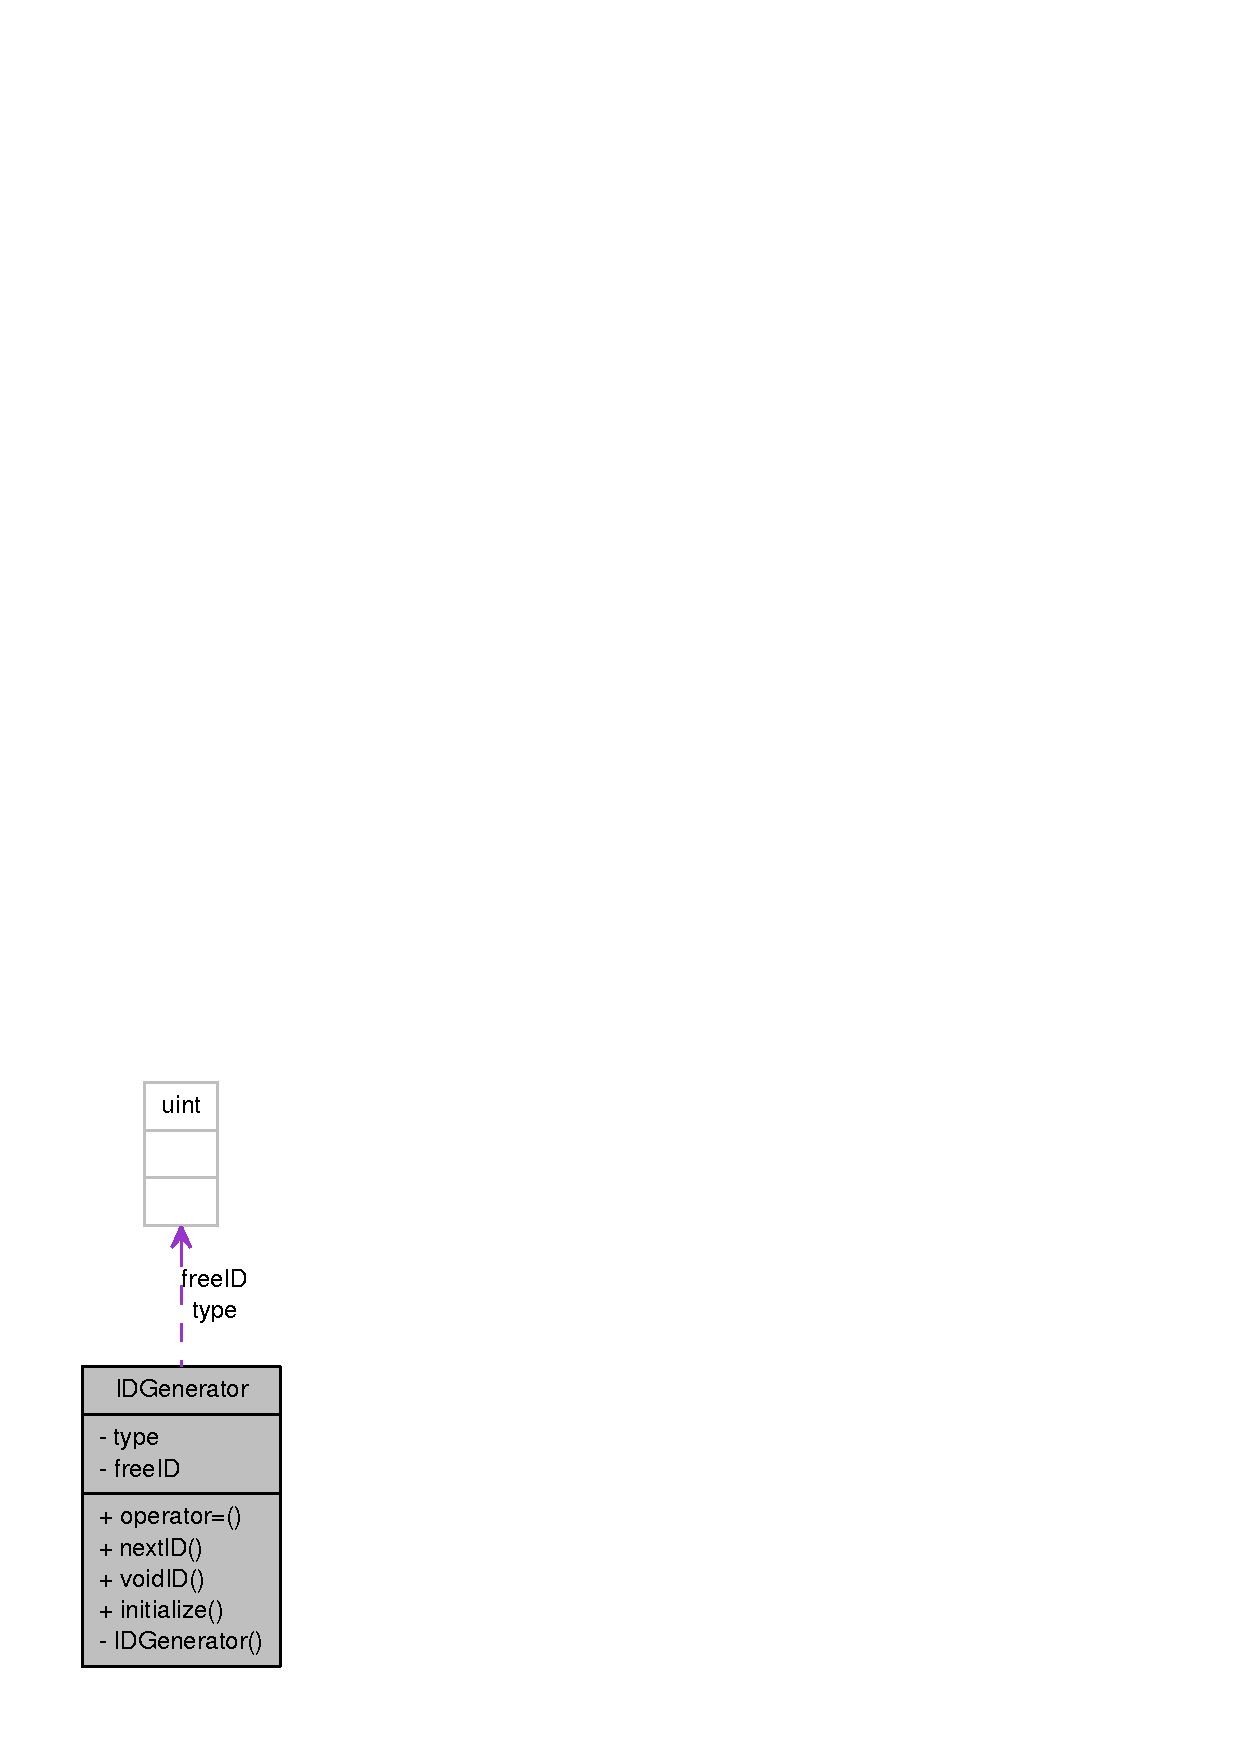
\includegraphics[width=138pt]{classIDGenerator__coll__graph}
\end{center}
\end{figure}
\subsection*{Komponenty}
\begin{DoxyCompactItemize}
\item 
class \hyperlink{classIDGenerator_1_1ID}{ID}
\begin{DoxyCompactList}\small\item\em Obiekt reprezentuje dany identyfikator określonego typu. \item\end{DoxyCompactList}\end{DoxyCompactItemize}
\subsection*{Metody publiczne}
\begin{DoxyCompactItemize}
\item 
\hyperlink{classIDGenerator}{IDGenerator} \& \hyperlink{classIDGenerator_a1cead736be7f5fae000fe1c5f225234b}{operator=} (const \hyperlink{classIDGenerator}{IDGenerator} \&o)  throw (char$\ast$)
\begin{DoxyCompactList}\small\item\em Przeładowany operator przypisania dla upewnienia się, że żaden generator nie zostanie zniszczony. \item\end{DoxyCompactList}\item 
\hyperlink{classIDGenerator_1_1ID}{ID} \hyperlink{classIDGenerator_a5e7eba106b14d8d09974bb6330476926}{nextID} ()
\begin{DoxyCompactList}\small\item\em Generuje następny identyfikator. \item\end{DoxyCompactList}\item 
\hyperlink{classIDGenerator_1_1ID}{ID} \hyperlink{classIDGenerator_ad5c8d7b639350d1f19dd990d850179c1}{voidID} ()
\begin{DoxyCompactList}\small\item\em Generuje niezainicjalizowany identyfikator. \item\end{DoxyCompactList}\item 
void \hyperlink{classIDGenerator_a16c5cba9a30dc95d05b72a1253fb54b2}{initialize} ()  throw (char$\ast$)
\begin{DoxyCompactList}\small\item\em Inicjalizuje dany generator identyfikatorów. \item\end{DoxyCompactList}\end{DoxyCompactItemize}
\subsection*{Metody prywatne}
\begin{DoxyCompactItemize}
\item 
\hyperlink{classIDGenerator_a9211b96bb2de7ec0479483c04b0263a5}{IDGenerator} (uint T)
\begin{DoxyCompactList}\small\item\em Inicjalizuje dany generator. \item\end{DoxyCompactList}\end{DoxyCompactItemize}
\subsection*{Atrybuty prywatne}
\begin{DoxyCompactItemize}
\item 
uint \hyperlink{classIDGenerator_abe469295c859bc2edc533a190ae2e1d9}{type}
\begin{DoxyCompactList}\small\item\em Typ identyfikatorów generowanych przez dany generator. \item\end{DoxyCompactList}\item 
uint \hyperlink{classIDGenerator_a5685b28917288954557a222cab550298}{freeID}
\begin{DoxyCompactList}\small\item\em Pierwszy wolny \hyperlink{classIDGenerator_1_1ID}{ID}. \item\end{DoxyCompactList}\end{DoxyCompactItemize}
\subsection*{Przyjaciele}
\begin{DoxyCompactItemize}
\item 
class \hyperlink{classIDGenerator_ab840f4c248c2a91409f520e48e774cfb}{GeneratorIDGenerator}
\begin{DoxyCompactList}\small\item\em Każdy generator identyfikatorów jest zaprzyjaźniony ze swoim stwórcą. \item\end{DoxyCompactList}\item 
QDataStream \& \hyperlink{classIDGenerator_a244688be6d84ec73612ddd66ab376bd1}{operator$<$$<$} (QDataStream \&stream, const \hyperlink{classIDGenerator}{IDGenerator} \&generator)
\begin{DoxyCompactList}\small\item\em Zapisuje dany generator identyfikatorów do danego strumienia. \item\end{DoxyCompactList}\item 
QDataStream \& \hyperlink{classIDGenerator_a4f86069b5b5ede60ff2e613fbcf10de4}{operator$>$$>$} (QDataStream \&stream, \hyperlink{classIDGenerator}{IDGenerator} \&generator)
\begin{DoxyCompactList}\small\item\em Odczytuje dany generator identyfikatorów z danego strumienia. \item\end{DoxyCompactList}\end{DoxyCompactItemize}


\subsection{Opis szczegółowy}
Generator identyfikatorów określonego typu. 

Definicja w linii 8 pliku idgenerator.h.



\subsection{Dokumentacja konstruktora i destruktora}
\hypertarget{classIDGenerator_a9211b96bb2de7ec0479483c04b0263a5}{
\index{IDGenerator@{IDGenerator}!IDGenerator@{IDGenerator}}
\index{IDGenerator@{IDGenerator}!IDGenerator@{IDGenerator}}
\subsubsection[{IDGenerator}]{\setlength{\rightskip}{0pt plus 5cm}IDGenerator::IDGenerator (uint {\em T})\hspace{0.3cm}{\ttfamily  \mbox{[}inline, private\mbox{]}}}}
\label{classIDGenerator_a9211b96bb2de7ec0479483c04b0263a5}


Inicjalizuje dany generator. 


\begin{DoxyParams}{Parametry}
\item[{\em T}]Typ identyfikatorów generowanych przez ten generator. \end{DoxyParams}


Definicja w linii 91 pliku idgenerator.h.




\begin{DoxyCode}
91 : type(T), freeID(1) {}
\end{DoxyCode}




\subsection{Dokumentacja funkcji składowych}
\hypertarget{classIDGenerator_a16c5cba9a30dc95d05b72a1253fb54b2}{
\index{IDGenerator@{IDGenerator}!initialize@{initialize}}
\index{initialize@{initialize}!IDGenerator@{IDGenerator}}
\subsubsection[{initialize}]{\setlength{\rightskip}{0pt plus 5cm}void IDGenerator::initialize ()  throw (char$\ast$)}}
\label{classIDGenerator_a16c5cba9a30dc95d05b72a1253fb54b2}


Inicjalizuje dany generator identyfikatorów. 

Inicjalizowany identyfikator MUSI być niezainicjalizowany! 

Definicja w linii 4 pliku idgenerator.cpp.



Odwołuje się do GeneratorIDGenerator::nextIDGenerator() i type.




\begin{DoxyCode}
5 {
6     if (type!=0)
7         throw "Error";
8     *this=GeneratorIDGenerator::nextIDGenerator();
9 }
\end{DoxyCode}




Oto graf wywołań dla tej funkcji:\nopagebreak
\begin{figure}[H]
\begin{center}
\leavevmode
\includegraphics[width=216pt]{classIDGenerator_a16c5cba9a30dc95d05b72a1253fb54b2_cgraph}
\end{center}
\end{figure}


\hypertarget{classIDGenerator_a5e7eba106b14d8d09974bb6330476926}{
\index{IDGenerator@{IDGenerator}!nextID@{nextID}}
\index{nextID@{nextID}!IDGenerator@{IDGenerator}}
\subsubsection[{nextID}]{\setlength{\rightskip}{0pt plus 5cm}{\bf ID} IDGenerator::nextID ()\hspace{0.3cm}{\ttfamily  \mbox{[}inline\mbox{]}}}}
\label{classIDGenerator_a5e7eba106b14d8d09974bb6330476926}


Generuje następny identyfikator. 



Definicja w linii 72 pliku idgenerator.h.



Odwołuje się do freeID i type.



Odwołania w main().




\begin{DoxyCode}
73     {
74         return ID(freeID++,type);
75     }
\end{DoxyCode}




Oto graf wywoływań tej funkcji:\nopagebreak
\begin{figure}[H]
\begin{center}
\leavevmode
\includegraphics[width=121pt]{classIDGenerator_a5e7eba106b14d8d09974bb6330476926_icgraph}
\end{center}
\end{figure}


\hypertarget{classIDGenerator_a1cead736be7f5fae000fe1c5f225234b}{
\index{IDGenerator@{IDGenerator}!operator=@{operator=}}
\index{operator=@{operator=}!IDGenerator@{IDGenerator}}
\subsubsection[{operator=}]{\setlength{\rightskip}{0pt plus 5cm}{\bf IDGenerator} \& IDGenerator::operator= (const {\bf IDGenerator} \& {\em o})  throw (char$\ast$)}}
\label{classIDGenerator_a1cead736be7f5fae000fe1c5f225234b}


Przeładowany operator przypisania dla upewnienia się, że żaden generator nie zostanie zniszczony. 



Definicja w linii 11 pliku idgenerator.cpp.



Odwołuje się do type.




\begin{DoxyCode}
12 {
13     if (type!=0)
14         throw "Error";
15     type=o.type;
16     freeID=o.freeID;
17     return *this;
18 }
\end{DoxyCode}


\hypertarget{classIDGenerator_ad5c8d7b639350d1f19dd990d850179c1}{
\index{IDGenerator@{IDGenerator}!voidID@{voidID}}
\index{voidID@{voidID}!IDGenerator@{IDGenerator}}
\subsubsection[{voidID}]{\setlength{\rightskip}{0pt plus 5cm}{\bf ID} IDGenerator::voidID ()\hspace{0.3cm}{\ttfamily  \mbox{[}inline\mbox{]}}}}
\label{classIDGenerator_ad5c8d7b639350d1f19dd990d850179c1}


Generuje niezainicjalizowany identyfikator. 



Definicja w linii 78 pliku idgenerator.h.



Odwołuje się do type.




\begin{DoxyCode}
79     {
80         return ID(0,type);
81     }
\end{DoxyCode}




\subsection{Dokumentacja przyjaciół i funkcji związanych}
\hypertarget{classIDGenerator_ab840f4c248c2a91409f520e48e774cfb}{
\index{IDGenerator@{IDGenerator}!GeneratorIDGenerator@{GeneratorIDGenerator}}
\index{GeneratorIDGenerator@{GeneratorIDGenerator}!IDGenerator@{IDGenerator}}
\subsubsection[{GeneratorIDGenerator}]{\setlength{\rightskip}{0pt plus 5cm}friend class {\bf GeneratorIDGenerator}\hspace{0.3cm}{\ttfamily  \mbox{[}friend\mbox{]}}}}
\label{classIDGenerator_ab840f4c248c2a91409f520e48e774cfb}


Każdy generator identyfikatorów jest zaprzyjaźniony ze swoim stwórcą. 



Definicja w linii 11 pliku idgenerator.h.

\hypertarget{classIDGenerator_a244688be6d84ec73612ddd66ab376bd1}{
\index{IDGenerator@{IDGenerator}!operator$<$$<$@{operator$<$$<$}}
\index{operator$<$$<$@{operator$<$$<$}!IDGenerator@{IDGenerator}}
\subsubsection[{operator$<$$<$}]{\setlength{\rightskip}{0pt plus 5cm}QDataStream\& operator$<$$<$ (QDataStream \& {\em stream}, \/  const {\bf IDGenerator} \& {\em generator})\hspace{0.3cm}{\ttfamily  \mbox{[}friend\mbox{]}}}}
\label{classIDGenerator_a244688be6d84ec73612ddd66ab376bd1}


Zapisuje dany generator identyfikatorów do danego strumienia. 


\begin{DoxyParams}{Parametry}
\item[{\em stream}]Strumień do którego będzie zapisany generator identyfikatorów. \item[{\em generator}]Generator identyfikatorów który zostanie zapisany. \end{DoxyParams}
\begin{DoxyReturn}{Zwraca}
Ten sam strumień. 
\end{DoxyReturn}


Definicja w linii 30 pliku idgenerator.cpp.




\begin{DoxyCode}
31 {
32     return stream<<generator.type<<generator.freeID;
33 }
\end{DoxyCode}


\hypertarget{classIDGenerator_a4f86069b5b5ede60ff2e613fbcf10de4}{
\index{IDGenerator@{IDGenerator}!operator$>$$>$@{operator$>$$>$}}
\index{operator$>$$>$@{operator$>$$>$}!IDGenerator@{IDGenerator}}
\subsubsection[{operator$>$$>$}]{\setlength{\rightskip}{0pt plus 5cm}QDataStream\& operator$>$$>$ (QDataStream \& {\em stream}, \/  {\bf IDGenerator} \& {\em generator})\hspace{0.3cm}{\ttfamily  \mbox{[}friend\mbox{]}}}}
\label{classIDGenerator_a4f86069b5b5ede60ff2e613fbcf10de4}


Odczytuje dany generator identyfikatorów z danego strumienia. 


\begin{DoxyParams}{Parametry}
\item[{\em stream}]Strumień z którego będzie odczytany generator identyfikatorów. \item[{\em generator}]Generator identyfikatorów który zostanie zainicjalizowany odczytanymi danymi. \end{DoxyParams}
\begin{DoxyReturn}{Zwraca}
Ten sam strumień. 
\end{DoxyReturn}


Definicja w linii 35 pliku idgenerator.cpp.




\begin{DoxyCode}
36 {
37     return stream>>generator.type>>generator.freeID;
38 }
\end{DoxyCode}




\subsection{Dokumentacja atrybutów składowych}
\hypertarget{classIDGenerator_a5685b28917288954557a222cab550298}{
\index{IDGenerator@{IDGenerator}!freeID@{freeID}}
\index{freeID@{freeID}!IDGenerator@{IDGenerator}}
\subsubsection[{freeID}]{\setlength{\rightskip}{0pt plus 5cm}uint {\bf IDGenerator::freeID}\hspace{0.3cm}{\ttfamily  \mbox{[}private\mbox{]}}}}
\label{classIDGenerator_a5685b28917288954557a222cab550298}


Pierwszy wolny \hyperlink{classIDGenerator_1_1ID}{ID}. 



Definicja w linii 65 pliku idgenerator.h.



Odwołania w nextID(), operator$<$$<$() i operator$>$$>$().

\hypertarget{classIDGenerator_abe469295c859bc2edc533a190ae2e1d9}{
\index{IDGenerator@{IDGenerator}!type@{type}}
\index{type@{type}!IDGenerator@{IDGenerator}}
\subsubsection[{type}]{\setlength{\rightskip}{0pt plus 5cm}uint {\bf IDGenerator::type}\hspace{0.3cm}{\ttfamily  \mbox{[}private\mbox{]}}}}
\label{classIDGenerator_abe469295c859bc2edc533a190ae2e1d9}


Typ identyfikatorów generowanych przez dany generator. 



Definicja w linii 64 pliku idgenerator.h.



Odwołania w initialize(), nextID(), operator$<$$<$(), operator=(), operator$>$$>$() i voidID().



Dokumentacja dla tej klasy została wygenerowana z plików:\begin{DoxyCompactItemize}
\item 
include/\hyperlink{idgenerator_8h}{idgenerator.h}\item 
src/\hyperlink{idgenerator_8cpp}{idgenerator.cpp}\end{DoxyCompactItemize}

\hypertarget{classobsolete_1_1MarkID}{
\section{Dokumentacja klasy obsolete::MarkID}
\label{classobsolete_1_1MarkID}\index{obsolete::MarkID@{obsolete::MarkID}}
}


Klasa reprezentująca identyfikator oceny.  




{\ttfamily \#include $<$markid.h$>$}



Diagram dziedziczenia dla obsolete::MarkID\nopagebreak
\begin{figure}[H]
\begin{center}
\leavevmode
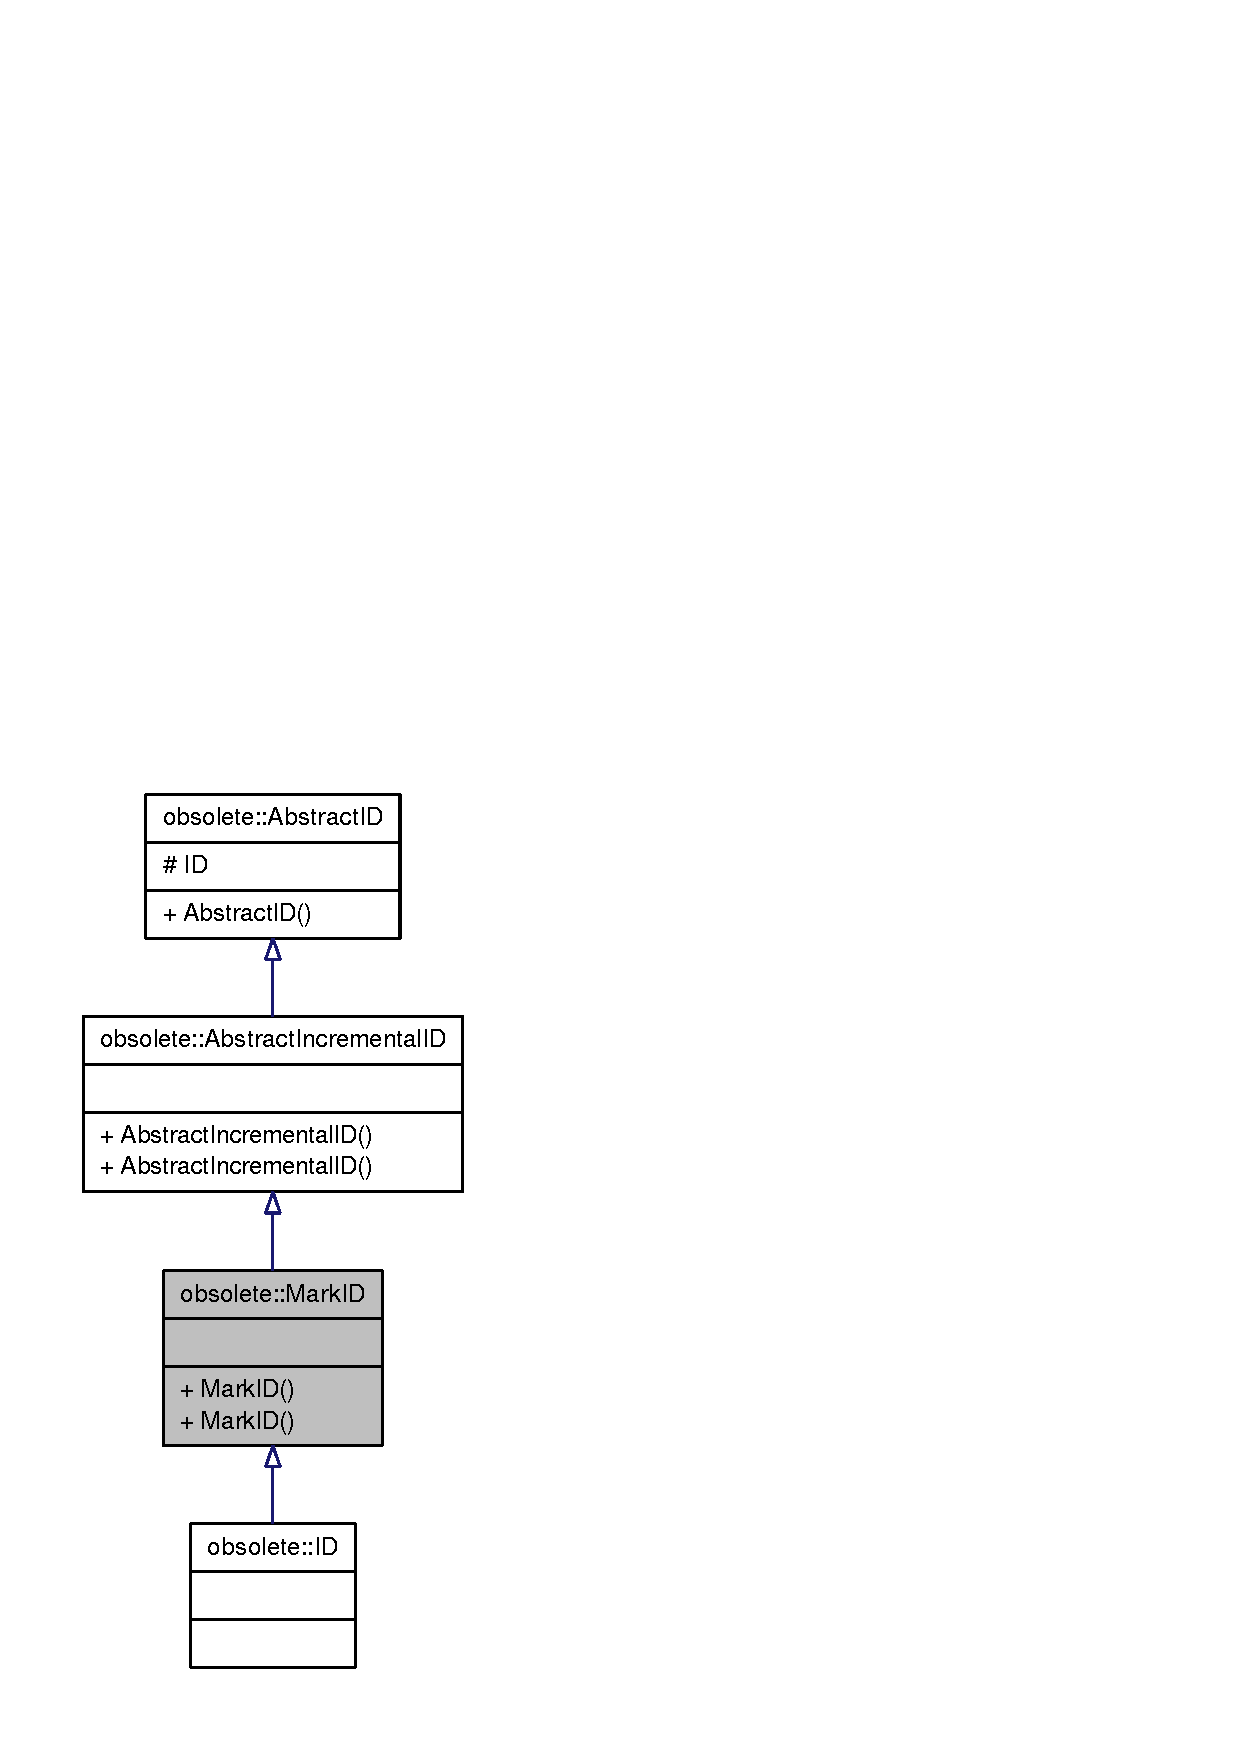
\includegraphics[height=400pt]{classobsolete_1_1MarkID__inherit__graph}
\end{center}
\end{figure}


Diagram współpracy dla obsolete::MarkID:\nopagebreak
\begin{figure}[H]
\begin{center}
\leavevmode
\includegraphics[height=400pt]{classobsolete_1_1MarkID__coll__graph}
\end{center}
\end{figure}
\subsection*{Metody publiczne}
\begin{DoxyCompactItemize}
\item 
\hyperlink{classobsolete_1_1MarkID_a451629e8562c9b4283835873d0416966}{MarkID} (uint \hyperlink{classobsolete_1_1ID}{ID})
\begin{DoxyCompactList}\small\item\em Wykorzystuje konstruktor klasy nadrzędnej. \item\end{DoxyCompactList}\item 
\hyperlink{classobsolete_1_1MarkID_a255fecd21149b8421bab3be478b821c9}{MarkID} ()
\begin{DoxyCompactList}\small\item\em Pozwalam również na tworzenie niezainicjalizowanych obiektów. \item\end{DoxyCompactList}\end{DoxyCompactItemize}
\subsection*{Atrybuty chronione}
\begin{DoxyCompactItemize}
\item 
uint \hyperlink{classobsolete_1_1AbstractID_a5f67fa1c7d96085f0ef41193b60b570c}{ID}
\begin{DoxyCompactList}\small\item\em Reprezentowany \hyperlink{classobsolete_1_1ID}{ID}. \item\end{DoxyCompactList}\end{DoxyCompactItemize}


\subsection{Opis szczegółowy}
Klasa reprezentująca identyfikator oceny. 

Definicja w linii 10 pliku markid.h.



\subsection{Dokumentacja konstruktora i destruktora}
\hypertarget{classobsolete_1_1MarkID_a451629e8562c9b4283835873d0416966}{
\index{obsolete::MarkID@{obsolete::MarkID}!MarkID@{MarkID}}
\index{MarkID@{MarkID}!obsolete::MarkID@{obsolete::MarkID}}
\subsubsection[{MarkID}]{\setlength{\rightskip}{0pt plus 5cm}obsolete::MarkID::MarkID (uint {\em ID})\hspace{0.3cm}{\ttfamily  \mbox{[}inline\mbox{]}}}}
\label{classobsolete_1_1MarkID_a451629e8562c9b4283835873d0416966}


Wykorzystuje konstruktor klasy nadrzędnej. 



Definicja w linii 13 pliku markid.h.

\hypertarget{classobsolete_1_1MarkID_a255fecd21149b8421bab3be478b821c9}{
\index{obsolete::MarkID@{obsolete::MarkID}!MarkID@{MarkID}}
\index{MarkID@{MarkID}!obsolete::MarkID@{obsolete::MarkID}}
\subsubsection[{MarkID}]{\setlength{\rightskip}{0pt plus 5cm}obsolete::MarkID::MarkID ()\hspace{0.3cm}{\ttfamily  \mbox{[}inline\mbox{]}}}}
\label{classobsolete_1_1MarkID_a255fecd21149b8421bab3be478b821c9}


Pozwalam również na tworzenie niezainicjalizowanych obiektów. 



Definicja w linii 14 pliku markid.h.



\subsection{Dokumentacja atrybutów składowych}
\hypertarget{classobsolete_1_1AbstractID_a5f67fa1c7d96085f0ef41193b60b570c}{
\index{obsolete::MarkID@{obsolete::MarkID}!ID@{ID}}
\index{ID@{ID}!obsolete::MarkID@{obsolete::MarkID}}
\subsubsection[{ID}]{\setlength{\rightskip}{0pt plus 5cm}uint {\bf obsolete::AbstractID::ID}\hspace{0.3cm}{\ttfamily  \mbox{[}protected, inherited\mbox{]}}}}
\label{classobsolete_1_1AbstractID_a5f67fa1c7d96085f0ef41193b60b570c}


Reprezentowany \hyperlink{classobsolete_1_1ID}{ID}. 



Definicja w linii 34 pliku abstractid.h.



Dokumentacja dla tej klasy została wygenerowana z pliku:\begin{DoxyCompactItemize}
\item 
include/obsolete/\hyperlink{markid_8h}{markid.h}\end{DoxyCompactItemize}

\hypertarget{classobsolete_1_1MarkIDGenerator}{
\section{Dokumentacja klasy obsolete::MarkIDGenerator}
\label{classobsolete_1_1MarkIDGenerator}\index{obsolete::MarkIDGenerator@{obsolete::MarkIDGenerator}}
}


Klasa generatorów generatorów identyfikatorów skutków wydarzeń.  




{\ttfamily \#include $<$markidgenerator.h$>$}



Diagram dziedziczenia dla obsolete::MarkIDGenerator\nopagebreak
\begin{figure}[H]
\begin{center}
\leavevmode
\includegraphics[width=218pt]{classobsolete_1_1MarkIDGenerator__inherit__graph}
\end{center}
\end{figure}


Diagram współpracy dla obsolete::MarkIDGenerator:\nopagebreak
\begin{figure}[H]
\begin{center}
\leavevmode
\includegraphics[height=400pt]{classobsolete_1_1MarkIDGenerator__coll__graph}
\end{center}
\end{figure}
\subsection*{Metody publiczne}
\begin{DoxyCompactItemize}
\item 
virtual \hyperlink{classobsolete_1_1ID}{ID} \hyperlink{classobsolete_1_1AbstractIDGenerator_a39d2f0147e3a028fef8299770e23db90}{createID} ()
\begin{DoxyCompactList}\small\item\em Tworzy nowy identyfikator. \item\end{DoxyCompactList}\end{DoxyCompactItemize}
\subsection*{Statyczne metody publiczne}
\begin{DoxyCompactItemize}
\item 
static \hyperlink{classobsolete_1_1ID}{ID} \hyperlink{classobsolete_1_1AbstractIDGenerator_a330da88ba80820ca6ce0a29cbbab9e1b}{createVoidID} ()
\begin{DoxyCompactList}\small\item\em Tworzy niezainicjowany identyfikator. \item\end{DoxyCompactList}\end{DoxyCompactItemize}
\subsection*{Atrybuty chronione}
\begin{DoxyCompactItemize}
\item 
uint \hyperlink{classobsolete_1_1AbstractID_a5f67fa1c7d96085f0ef41193b60b570c}{ID}
\begin{DoxyCompactList}\small\item\em Reprezentowany \hyperlink{classobsolete_1_1ID}{ID}. \item\end{DoxyCompactList}\end{DoxyCompactItemize}


\subsection{Opis szczegółowy}
Klasa generatorów generatorów identyfikatorów skutków wydarzeń. 

Definicja w linii 10 pliku markidgenerator.h.



\subsection{Dokumentacja funkcji składowych}
\hypertarget{classobsolete_1_1AbstractIDGenerator_a39d2f0147e3a028fef8299770e23db90}{
\index{obsolete::MarkIDGenerator@{obsolete::MarkIDGenerator}!createID@{createID}}
\index{createID@{createID}!obsolete::MarkIDGenerator@{obsolete::MarkIDGenerator}}
\subsubsection[{createID}]{\setlength{\rightskip}{0pt plus 5cm}virtual {\bf ID} obsolete::AbstractIDGenerator::createID ()\hspace{0.3cm}{\ttfamily  \mbox{[}virtual, inherited\mbox{]}}}}
\label{classobsolete_1_1AbstractIDGenerator_a39d2f0147e3a028fef8299770e23db90}


Tworzy nowy identyfikator. 

\hypertarget{classobsolete_1_1AbstractIDGenerator_a330da88ba80820ca6ce0a29cbbab9e1b}{
\index{obsolete::MarkIDGenerator@{obsolete::MarkIDGenerator}!createVoidID@{createVoidID}}
\index{createVoidID@{createVoidID}!obsolete::MarkIDGenerator@{obsolete::MarkIDGenerator}}
\subsubsection[{createVoidID}]{\setlength{\rightskip}{0pt plus 5cm}static {\bf ID} obsolete::AbstractIDGenerator::createVoidID ()\hspace{0.3cm}{\ttfamily  \mbox{[}static, inherited\mbox{]}}}}
\label{classobsolete_1_1AbstractIDGenerator_a330da88ba80820ca6ce0a29cbbab9e1b}


Tworzy niezainicjowany identyfikator. 



\subsection{Dokumentacja atrybutów składowych}
\hypertarget{classobsolete_1_1AbstractID_a5f67fa1c7d96085f0ef41193b60b570c}{
\index{obsolete::MarkIDGenerator@{obsolete::MarkIDGenerator}!ID@{ID}}
\index{ID@{ID}!obsolete::MarkIDGenerator@{obsolete::MarkIDGenerator}}
\subsubsection[{ID}]{\setlength{\rightskip}{0pt plus 5cm}uint {\bf obsolete::AbstractID::ID}\hspace{0.3cm}{\ttfamily  \mbox{[}protected, inherited\mbox{]}}}}
\label{classobsolete_1_1AbstractID_a5f67fa1c7d96085f0ef41193b60b570c}


Reprezentowany \hyperlink{classobsolete_1_1ID}{ID}. 



Definicja w linii 34 pliku abstractid.h.



Dokumentacja dla tej klasy została wygenerowana z pliku:\begin{DoxyCompactItemize}
\item 
include/obsolete/\hyperlink{markidgenerator_8h}{markidgenerator.h}\end{DoxyCompactItemize}

\hypertarget{classQDate}{
\section{Dokumentacja klasy QDate}
\label{classQDate}\index{QDate@{QDate}}
}


Diagram dziedziczenia dla QDate\nopagebreak
\begin{figure}[H]
\begin{center}
\leavevmode
\includegraphics[width=106pt]{classQDate__inherit__graph}
\end{center}
\end{figure}


Dokumentacja dla tej klasy została wygenerowana z pliku:\begin{DoxyCompactItemize}
\item 
include/\hyperlink{term_8h}{term.h}\end{DoxyCompactItemize}

\hypertarget{classobsolete_1_1State}{
\section{Dokumentacja klasy obsolete::State}
\label{classobsolete_1_1State}\index{obsolete::State@{obsolete::State}}
}


Klasa przechowująca wszelkie informacje o stanie aplikacji, bazy danych i danych.  




{\ttfamily \#include $<$state.h$>$}



Diagram współpracy dla obsolete::State:\nopagebreak
\begin{figure}[H]
\begin{center}
\leavevmode
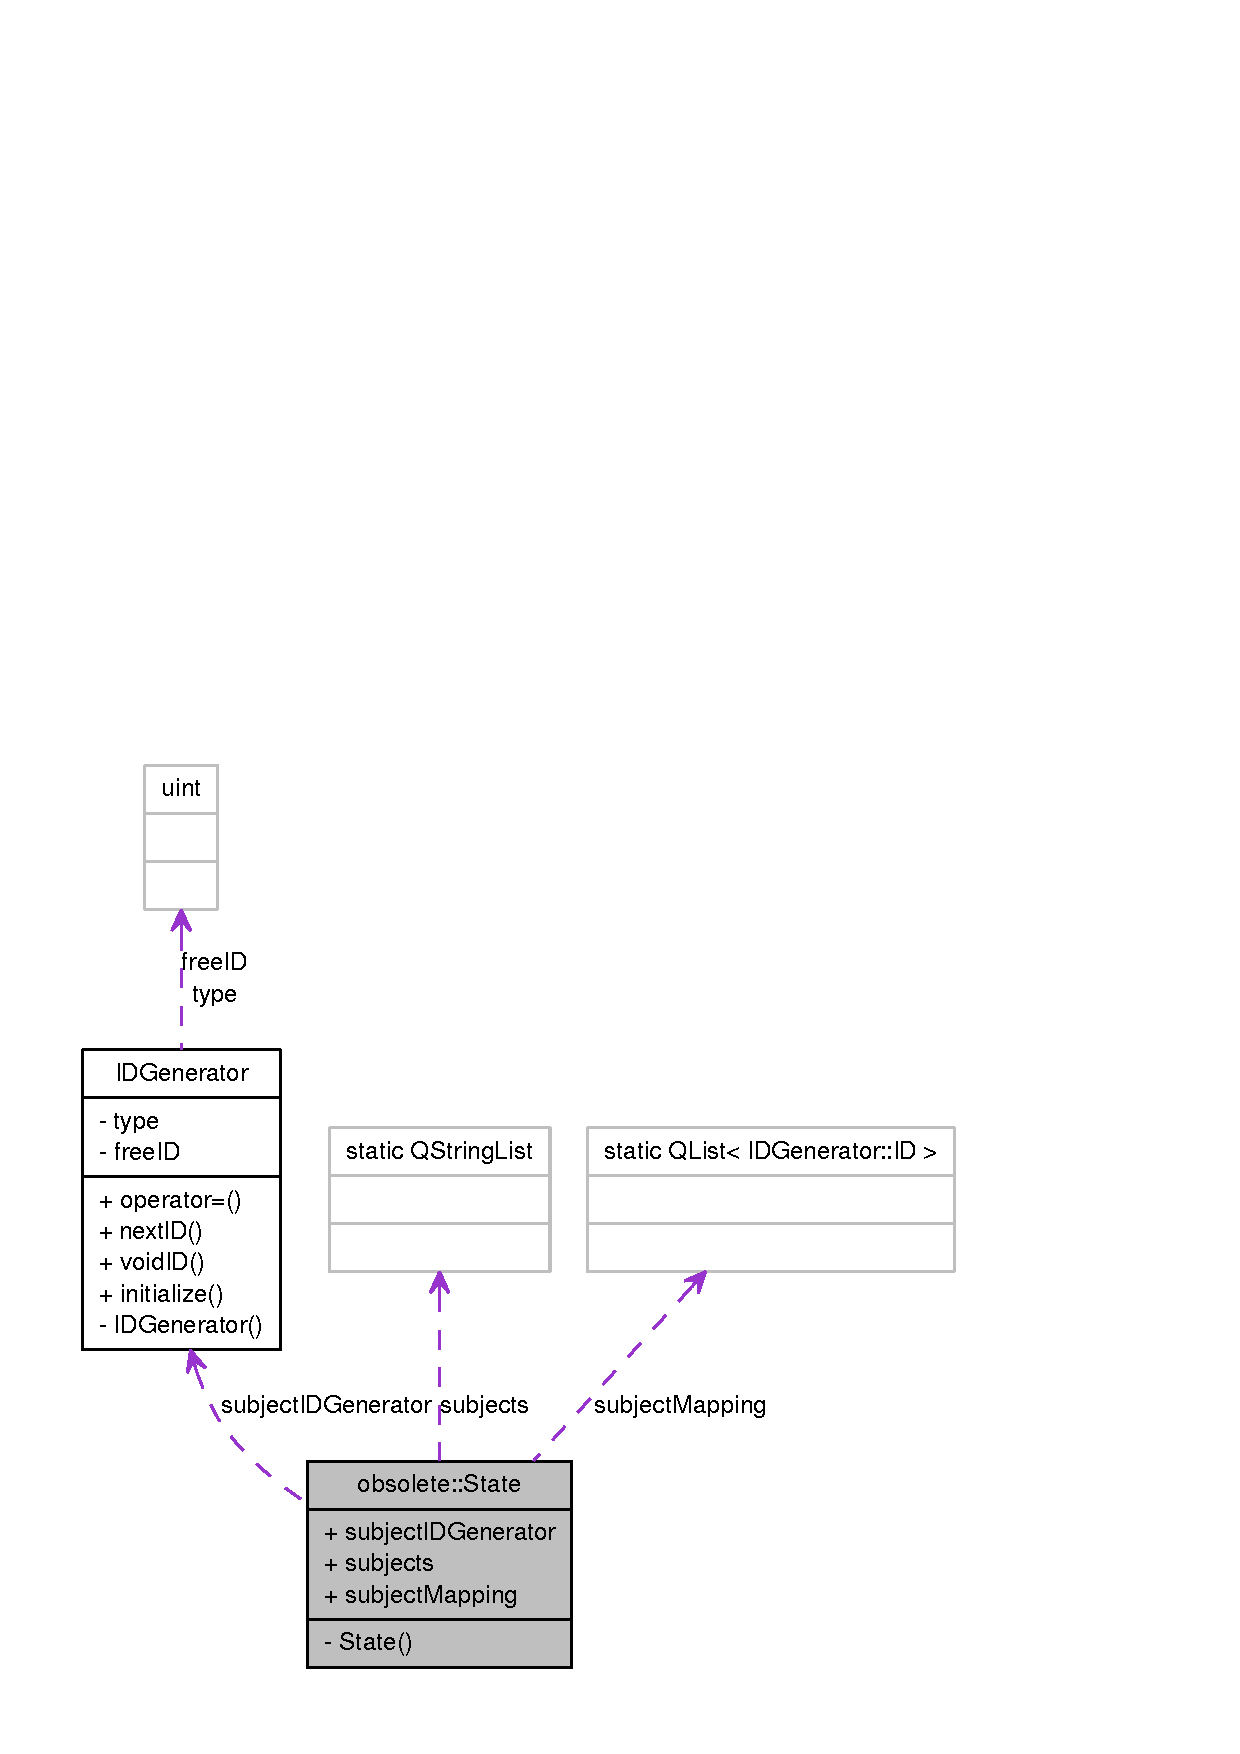
\includegraphics[width=400pt]{classobsolete_1_1State__coll__graph}
\end{center}
\end{figure}
\subsection*{Statyczne atrybuty publiczne}
\begin{DoxyCompactItemize}
\item 
static \hyperlink{classIDGenerator}{IDGenerator} \hyperlink{classobsolete_1_1State_a79baf22dac86724b99d4b2b785e38875}{subjectIDGenerator}
\begin{DoxyCompactList}\small\item\em Generator identyfikatorów przedmiotów. \item\end{DoxyCompactList}\item 
static QStringList \hyperlink{classobsolete_1_1State_aeaa49570838d7cd7bb5585385df92b1c}{subjects}
\begin{DoxyCompactList}\small\item\em Lista przedmiotów. subjects\mbox{[}\hyperlink{classobsolete_1_1SubjectID}{SubjectID}\mbox{]} = Przedmiot o zadanym identyfikatorze. \item\end{DoxyCompactList}\item 
static QList$<$ \hyperlink{classIDGenerator_1_1ID}{IDGenerator::ID} $>$ \hyperlink{classobsolete_1_1State_acbed5e9ef96a7bf365f2429e1384bd03}{subjectMapping}
\begin{DoxyCompactList}\small\item\em Lista odnośników \mbox{[}pozycja w ComboBox\mbox{]}-\/-\/$>$\mbox{[}pozycja w subjects\mbox{]}. \item\end{DoxyCompactList}\end{DoxyCompactItemize}
\subsection*{Metody prywatne}
\begin{DoxyCompactItemize}
\item 
\hyperlink{classobsolete_1_1State_ac8dd10c3b5045899fc6095b1c79d27d1}{State} ()
\begin{DoxyCompactList}\small\item\em Nie wolno tworzyć obiektów tej klasy. \item\end{DoxyCompactList}\end{DoxyCompactItemize}


\subsection{Opis szczegółowy}
Klasa przechowująca wszelkie informacje o stanie aplikacji, bazy danych i danych. Jest to kontener na informacje o przedmiotach.

Nie wolno tworzyć obiektów tej klasy, wszystkie pola są statyczne. 

Definicja w linii 15 pliku state.h.



\subsection{Dokumentacja konstruktora i destruktora}
\hypertarget{classobsolete_1_1State_ac8dd10c3b5045899fc6095b1c79d27d1}{
\index{obsolete::State@{obsolete::State}!State@{State}}
\index{State@{State}!obsolete::State@{obsolete::State}}
\subsubsection[{State}]{\setlength{\rightskip}{0pt plus 5cm}obsolete::State::State ()\hspace{0.3cm}{\ttfamily  \mbox{[}inline, private\mbox{]}}}}
\label{classobsolete_1_1State_ac8dd10c3b5045899fc6095b1c79d27d1}


Nie wolno tworzyć obiektów tej klasy. 



Definicja w linii 23 pliku state.h.



\subsection{Dokumentacja atrybutów składowych}
\hypertarget{classobsolete_1_1State_a79baf22dac86724b99d4b2b785e38875}{
\index{obsolete::State@{obsolete::State}!subjectIDGenerator@{subjectIDGenerator}}
\index{subjectIDGenerator@{subjectIDGenerator}!obsolete::State@{obsolete::State}}
\subsubsection[{subjectIDGenerator}]{\setlength{\rightskip}{0pt plus 5cm}{\bf IDGenerator} {\bf obsolete::State::subjectIDGenerator}\hspace{0.3cm}{\ttfamily  \mbox{[}static\mbox{]}}}}
\label{classobsolete_1_1State_a79baf22dac86724b99d4b2b785e38875}


Generator identyfikatorów przedmiotów. 



Definicja w linii 18 pliku state.h.

\hypertarget{classobsolete_1_1State_acbed5e9ef96a7bf365f2429e1384bd03}{
\index{obsolete::State@{obsolete::State}!subjectMapping@{subjectMapping}}
\index{subjectMapping@{subjectMapping}!obsolete::State@{obsolete::State}}
\subsubsection[{subjectMapping}]{\setlength{\rightskip}{0pt plus 5cm}QList$<${\bf IDGenerator::ID}$>$ {\bf obsolete::State::subjectMapping}\hspace{0.3cm}{\ttfamily  \mbox{[}static\mbox{]}}}}
\label{classobsolete_1_1State_acbed5e9ef96a7bf365f2429e1384bd03}


Lista odnośników \mbox{[}pozycja w ComboBox\mbox{]}-\/-\/$>$\mbox{[}pozycja w subjects\mbox{]}. 



Definicja w linii 20 pliku state.h.

\hypertarget{classobsolete_1_1State_aeaa49570838d7cd7bb5585385df92b1c}{
\index{obsolete::State@{obsolete::State}!subjects@{subjects}}
\index{subjects@{subjects}!obsolete::State@{obsolete::State}}
\subsubsection[{subjects}]{\setlength{\rightskip}{0pt plus 5cm}QStringList {\bf obsolete::State::subjects}\hspace{0.3cm}{\ttfamily  \mbox{[}static\mbox{]}}}}
\label{classobsolete_1_1State_aeaa49570838d7cd7bb5585385df92b1c}


Lista przedmiotów. subjects\mbox{[}\hyperlink{classobsolete_1_1SubjectID}{SubjectID}\mbox{]} = Przedmiot o zadanym identyfikatorze. 



Definicja w linii 19 pliku state.h.



Dokumentacja dla tej klasy została wygenerowana z pliku:\begin{DoxyCompactItemize}
\item 
include/obsolete/\hyperlink{state_8h}{state.h}\end{DoxyCompactItemize}

\hypertarget{classSubject}{
\section{Dokumentacja klasy Subject}
\label{classSubject}\index{Subject@{Subject}}
}


Reprezentuje informacje o pojedyńczym przedmiocie.  




{\ttfamily \#include $<$subject.h$>$}



Diagram współpracy dla Subject:\nopagebreak
\begin{figure}[H]
\begin{center}
\leavevmode
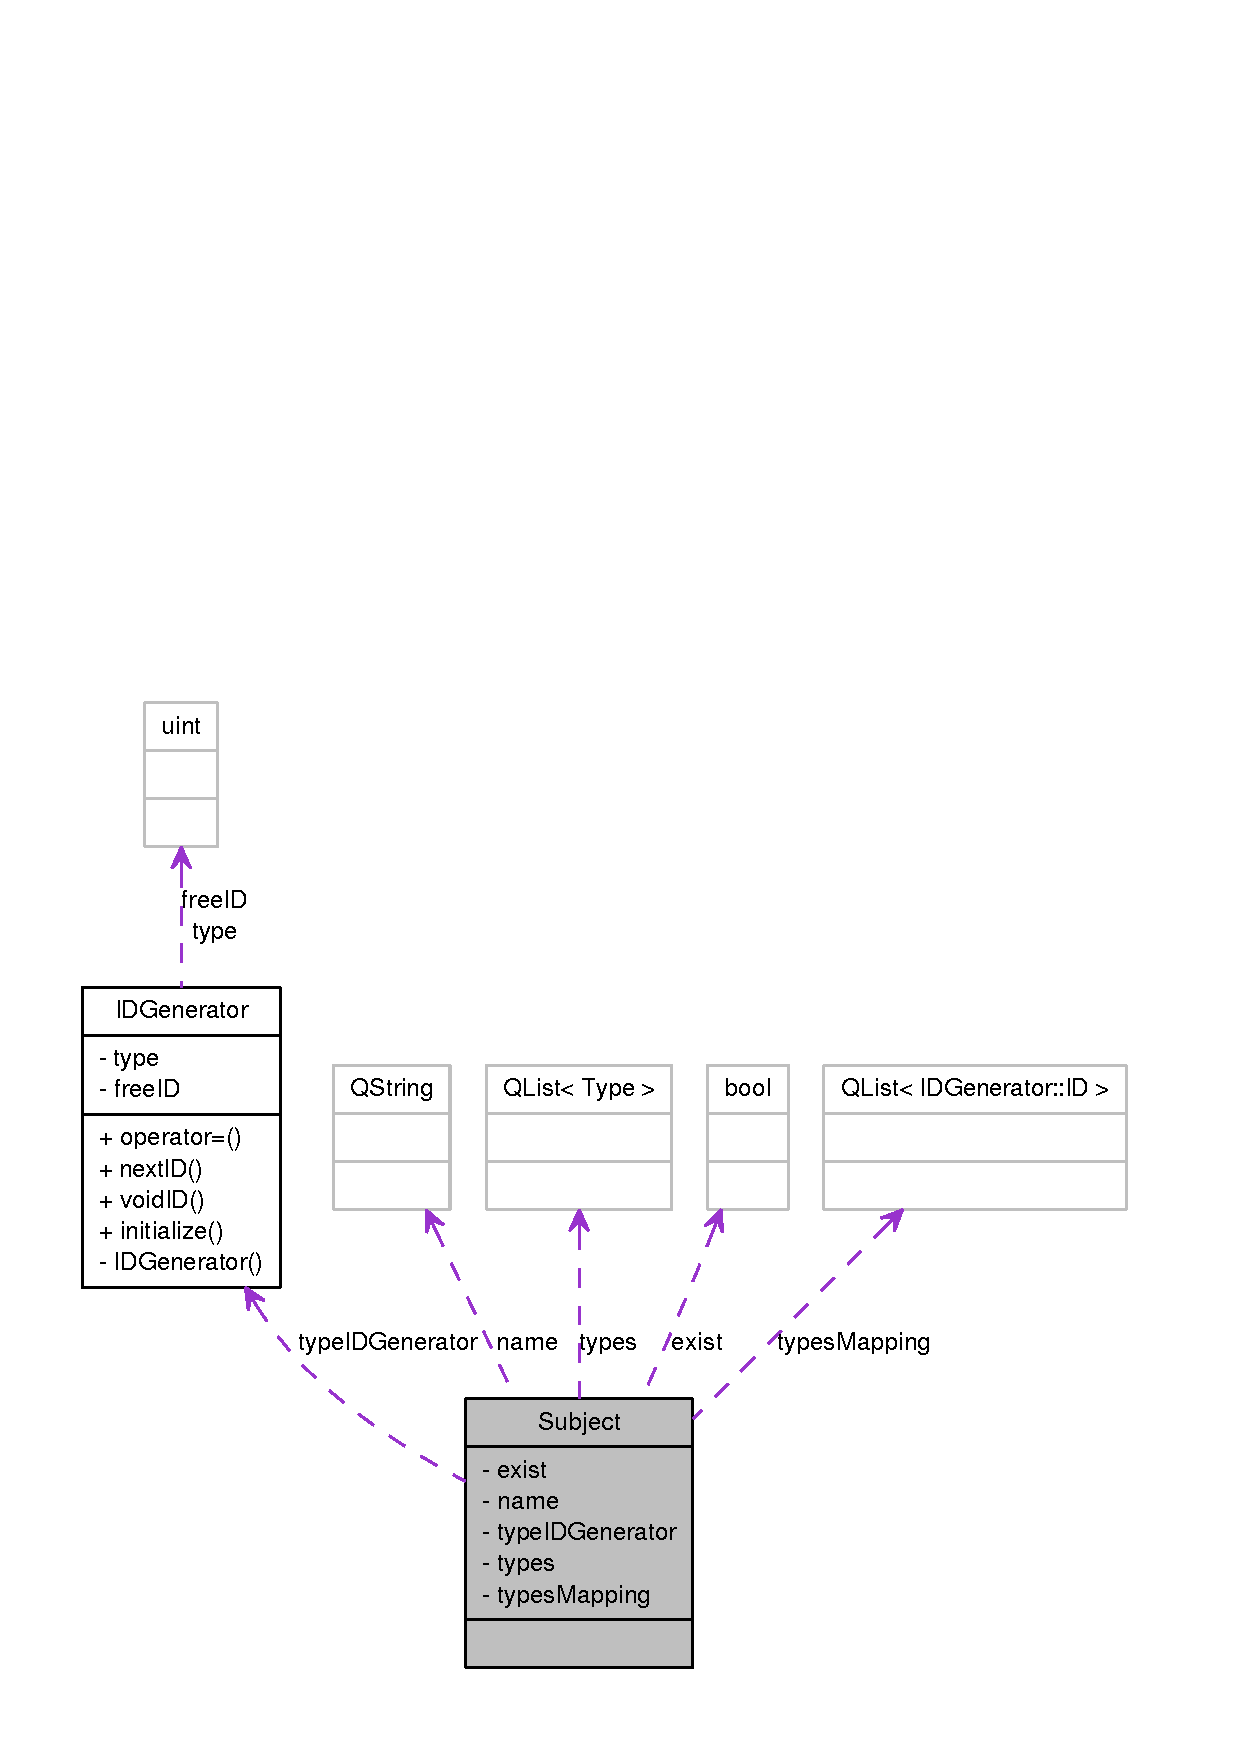
\includegraphics[width=400pt]{classSubject__coll__graph}
\end{center}
\end{figure}
\subsection*{Atrybuty prywatne}
\begin{DoxyCompactItemize}
\item 
bool \hyperlink{classSubject_a94220ae4e81cef6a54b3ad00c5189213}{exist}
\begin{DoxyCompactList}\small\item\em Czy ten obiekt reprezentuje dane. \item\end{DoxyCompactList}\item 
QString \hyperlink{classSubject_a816225e2744f102877f713f3123a6ba4}{name}
\begin{DoxyCompactList}\small\item\em Nazwa przedmiotu. \item\end{DoxyCompactList}\item 
\hyperlink{classIDGenerator}{IDGenerator} \hyperlink{classSubject_aab207d1dd2076df8de622c54d80fd8cd}{typeIDGenerator}
\begin{DoxyCompactList}\small\item\em Generator identyfikatorów typów wydarzeń. \item\end{DoxyCompactList}\item 
QList$<$ \hyperlink{classType}{Type} $>$ \hyperlink{classSubject_a05041c1516b065f1fb5f2c74c731a0a7}{types}
\begin{DoxyCompactList}\small\item\em Typy wydarzeń. Indeksowane types\mbox{[}TypeID\mbox{]} = wydarzenie TypeID. \item\end{DoxyCompactList}\item 
QList$<$ \hyperlink{classIDGenerator_1_1ID}{IDGenerator::ID} $>$ \hyperlink{classSubject_a986e6137767b698f8bdef30f24c32178}{typesMapping}
\begin{DoxyCompactList}\small\item\em Lista odnośników \mbox{[}pozycja w ComboBox\mbox{]}-\/-\/$>$\mbox{[}pozycja w types\mbox{]}. \item\end{DoxyCompactList}\end{DoxyCompactItemize}


\subsection{Opis szczegółowy}
Reprezentuje informacje o pojedyńczym przedmiocie. 

Definicja w linii 11 pliku subject.h.



\subsection{Dokumentacja atrybutów składowych}
\hypertarget{classSubject_a94220ae4e81cef6a54b3ad00c5189213}{
\index{Subject@{Subject}!exist@{exist}}
\index{exist@{exist}!Subject@{Subject}}
\subsubsection[{exist}]{\setlength{\rightskip}{0pt plus 5cm}bool {\bf Subject::exist}\hspace{0.3cm}{\ttfamily  \mbox{[}private\mbox{]}}}}
\label{classSubject_a94220ae4e81cef6a54b3ad00c5189213}


Czy ten obiekt reprezentuje dane. 



Definicja w linii 12 pliku subject.h.

\hypertarget{classSubject_a816225e2744f102877f713f3123a6ba4}{
\index{Subject@{Subject}!name@{name}}
\index{name@{name}!Subject@{Subject}}
\subsubsection[{name}]{\setlength{\rightskip}{0pt plus 5cm}QString {\bf Subject::name}\hspace{0.3cm}{\ttfamily  \mbox{[}private\mbox{]}}}}
\label{classSubject_a816225e2744f102877f713f3123a6ba4}


Nazwa przedmiotu. 



Definicja w linii 13 pliku subject.h.

\hypertarget{classSubject_aab207d1dd2076df8de622c54d80fd8cd}{
\index{Subject@{Subject}!typeIDGenerator@{typeIDGenerator}}
\index{typeIDGenerator@{typeIDGenerator}!Subject@{Subject}}
\subsubsection[{typeIDGenerator}]{\setlength{\rightskip}{0pt plus 5cm}{\bf IDGenerator} {\bf Subject::typeIDGenerator}\hspace{0.3cm}{\ttfamily  \mbox{[}private\mbox{]}}}}
\label{classSubject_aab207d1dd2076df8de622c54d80fd8cd}


Generator identyfikatorów typów wydarzeń. 



Definicja w linii 14 pliku subject.h.

\hypertarget{classSubject_a05041c1516b065f1fb5f2c74c731a0a7}{
\index{Subject@{Subject}!types@{types}}
\index{types@{types}!Subject@{Subject}}
\subsubsection[{types}]{\setlength{\rightskip}{0pt plus 5cm}QList$<${\bf Type}$>$ {\bf Subject::types}\hspace{0.3cm}{\ttfamily  \mbox{[}private\mbox{]}}}}
\label{classSubject_a05041c1516b065f1fb5f2c74c731a0a7}


Typy wydarzeń. Indeksowane types\mbox{[}TypeID\mbox{]} = wydarzenie TypeID. 



Definicja w linii 15 pliku subject.h.

\hypertarget{classSubject_a986e6137767b698f8bdef30f24c32178}{
\index{Subject@{Subject}!typesMapping@{typesMapping}}
\index{typesMapping@{typesMapping}!Subject@{Subject}}
\subsubsection[{typesMapping}]{\setlength{\rightskip}{0pt plus 5cm}QList$<${\bf IDGenerator::ID}$>$ {\bf Subject::typesMapping}\hspace{0.3cm}{\ttfamily  \mbox{[}private\mbox{]}}}}
\label{classSubject_a986e6137767b698f8bdef30f24c32178}


Lista odnośników \mbox{[}pozycja w ComboBox\mbox{]}-\/-\/$>$\mbox{[}pozycja w types\mbox{]}. 



Definicja w linii 16 pliku subject.h.



Dokumentacja dla tej klasy została wygenerowana z pliku:\begin{DoxyCompactItemize}
\item 
include/\hyperlink{subject_8h}{subject.h}\end{DoxyCompactItemize}

\hypertarget{classobsolete_1_1SubjectID}{
\section{Dokumentacja klasy obsolete::SubjectID}
\label{classobsolete_1_1SubjectID}\index{obsolete::SubjectID@{obsolete::SubjectID}}
}


Klasa reprezentująca identyfikator przedmiotu.  




{\ttfamily \#include $<$subjectid.h$>$}



Diagram dziedziczenia dla obsolete::SubjectID\nopagebreak
\begin{figure}[H]
\begin{center}
\leavevmode
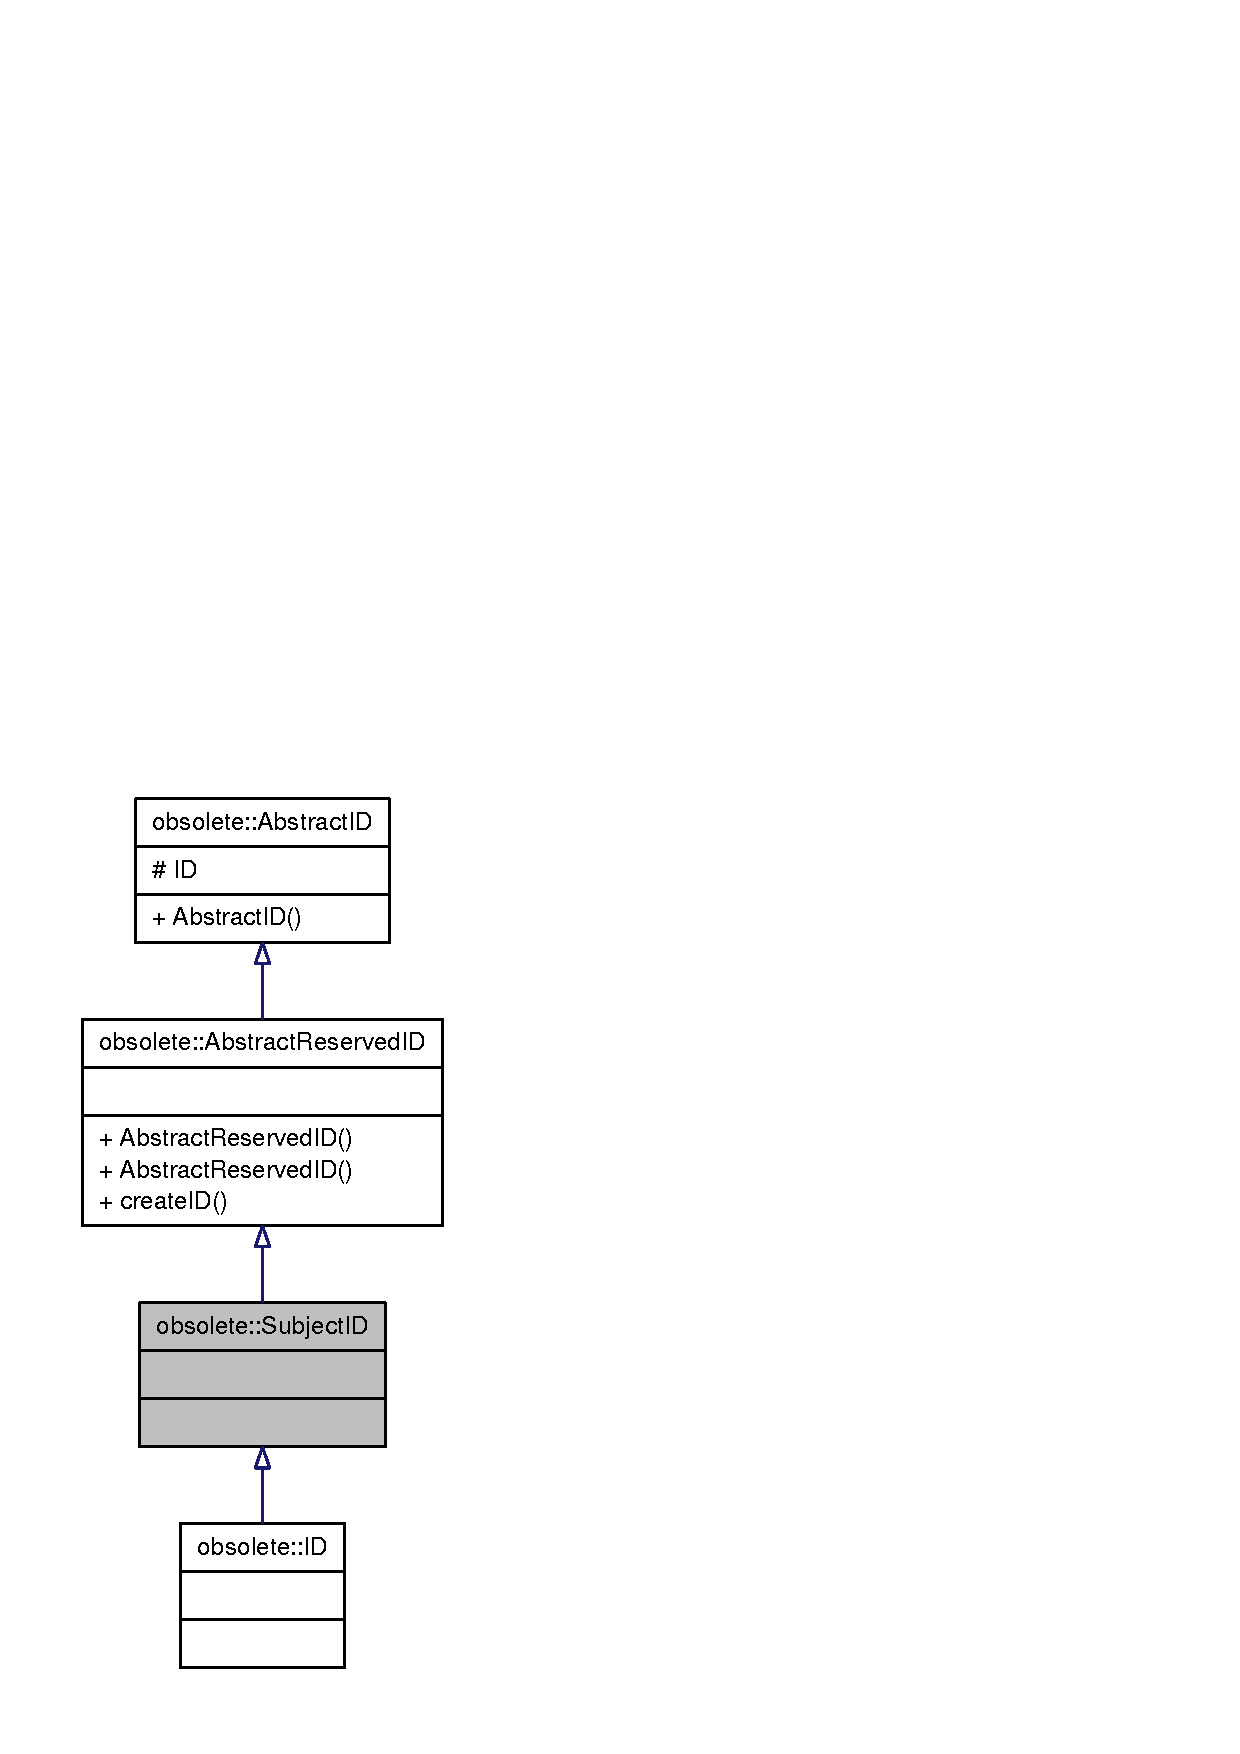
\includegraphics[height=400pt]{classobsolete_1_1SubjectID__inherit__graph}
\end{center}
\end{figure}


Diagram współpracy dla obsolete::SubjectID:\nopagebreak
\begin{figure}[H]
\begin{center}
\leavevmode
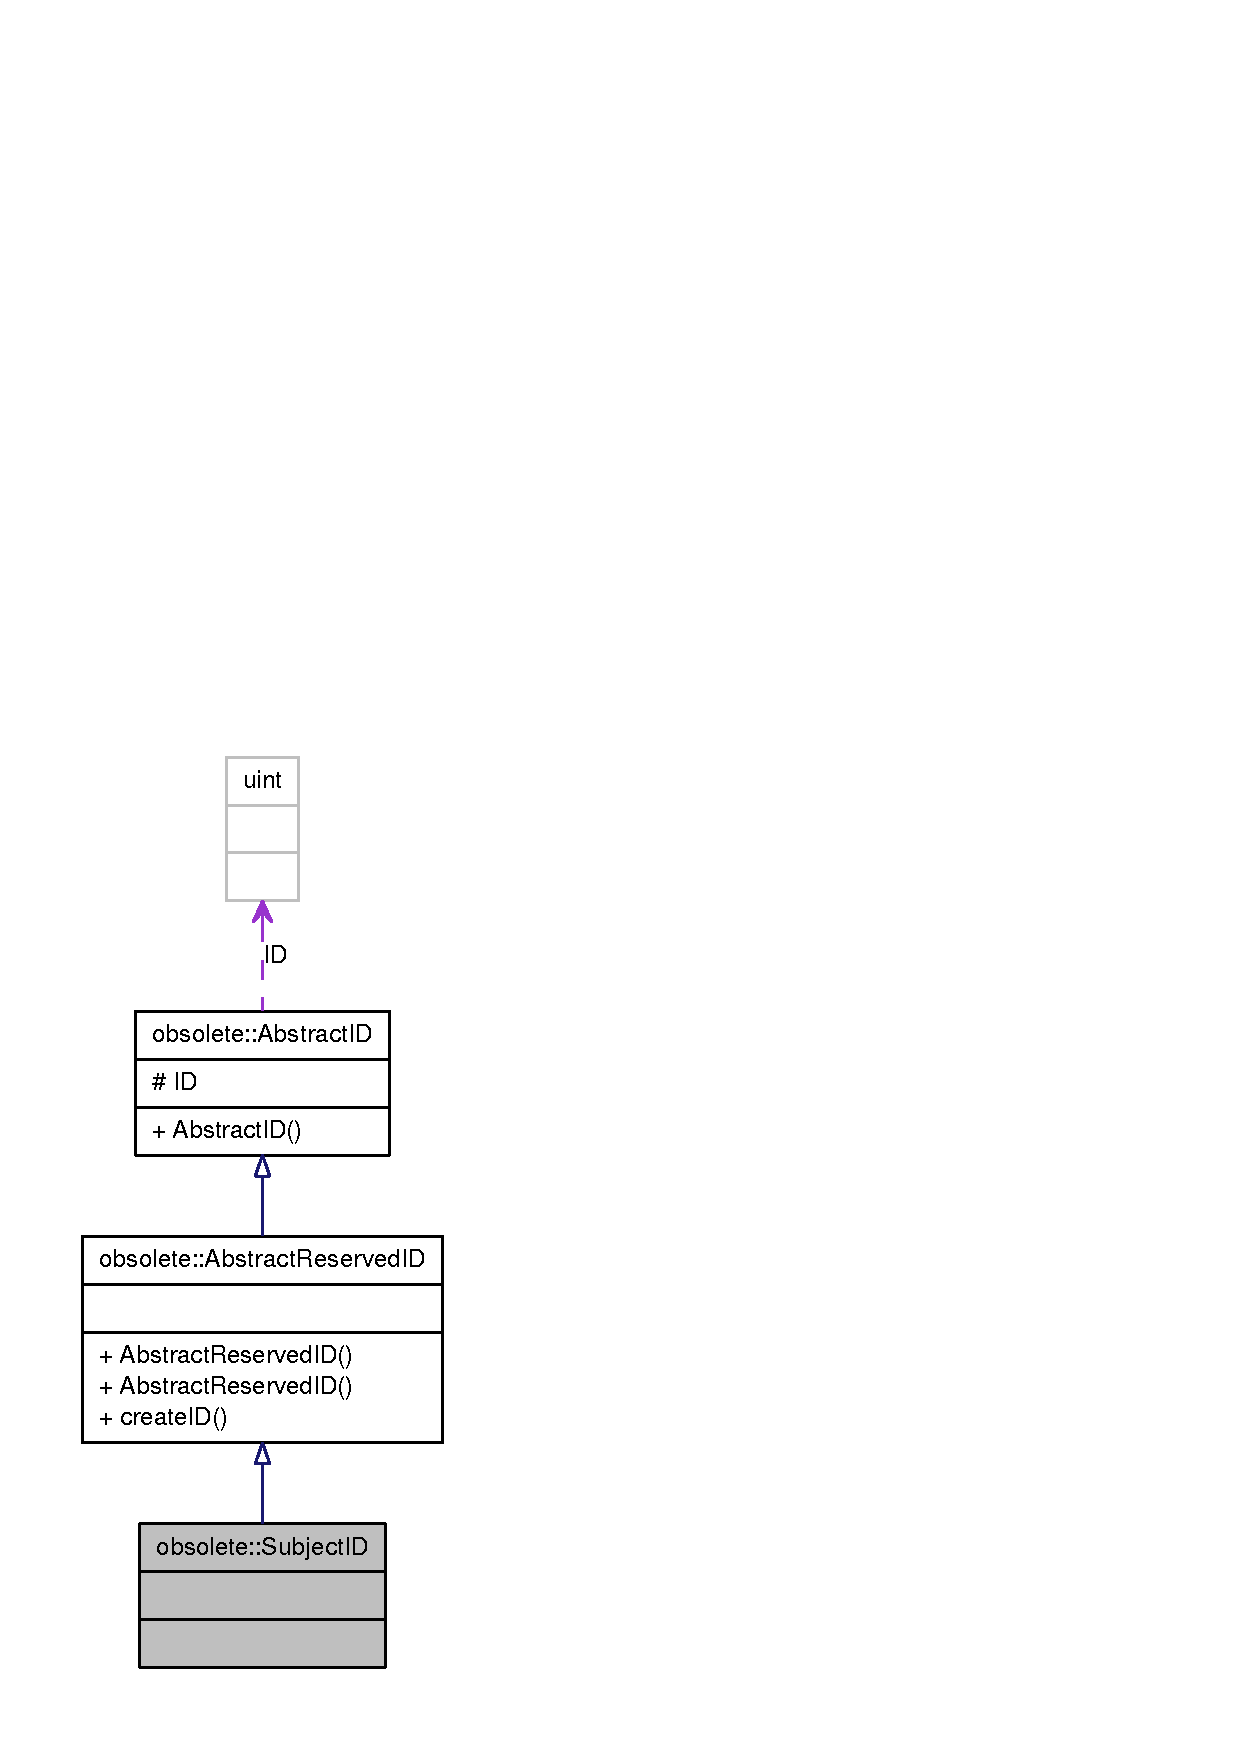
\includegraphics[height=400pt]{classobsolete_1_1SubjectID__coll__graph}
\end{center}
\end{figure}
\subsection*{Statyczne metody publiczne}
\begin{DoxyCompactItemize}
\item 
static \hyperlink{classobsolete_1_1AbstractReservedID}{AbstractReservedID} \hyperlink{classobsolete_1_1AbstractReservedID_a38fa00bf6097ab9cff285c8480c8097e}{createID} (uint \hyperlink{classobsolete_1_1ID}{ID})
\begin{DoxyCompactList}\small\item\em Opakowuje numer porządkowy zadaną liczbą. \item\end{DoxyCompactList}\end{DoxyCompactItemize}
\subsection*{Atrybuty chronione}
\begin{DoxyCompactItemize}
\item 
uint \hyperlink{classobsolete_1_1AbstractID_a5f67fa1c7d96085f0ef41193b60b570c}{ID}
\begin{DoxyCompactList}\small\item\em Reprezentowany \hyperlink{classobsolete_1_1ID}{ID}. \item\end{DoxyCompactList}\end{DoxyCompactItemize}


\subsection{Opis szczegółowy}
Klasa reprezentująca identyfikator przedmiotu. 

Definicja w linii 10 pliku subjectid.h.



\subsection{Dokumentacja funkcji składowych}
\hypertarget{classobsolete_1_1AbstractReservedID_a38fa00bf6097ab9cff285c8480c8097e}{
\index{obsolete::SubjectID@{obsolete::SubjectID}!createID@{createID}}
\index{createID@{createID}!obsolete::SubjectID@{obsolete::SubjectID}}
\subsubsection[{createID}]{\setlength{\rightskip}{0pt plus 5cm}static {\bf AbstractReservedID} obsolete::AbstractReservedID::createID (uint {\em ID})\hspace{0.3cm}{\ttfamily  \mbox{[}inline, static, inherited\mbox{]}}}}
\label{classobsolete_1_1AbstractReservedID_a38fa00bf6097ab9cff285c8480c8097e}


Opakowuje numer porządkowy zadaną liczbą. 



\subsection{Dokumentacja atrybutów składowych}
\hypertarget{classobsolete_1_1AbstractID_a5f67fa1c7d96085f0ef41193b60b570c}{
\index{obsolete::SubjectID@{obsolete::SubjectID}!ID@{ID}}
\index{ID@{ID}!obsolete::SubjectID@{obsolete::SubjectID}}
\subsubsection[{ID}]{\setlength{\rightskip}{0pt plus 5cm}uint {\bf obsolete::AbstractID::ID}\hspace{0.3cm}{\ttfamily  \mbox{[}protected, inherited\mbox{]}}}}
\label{classobsolete_1_1AbstractID_a5f67fa1c7d96085f0ef41193b60b570c}


Reprezentowany \hyperlink{classobsolete_1_1ID}{ID}. 



Definicja w linii 34 pliku abstractid.h.



Dokumentacja dla tej klasy została wygenerowana z pliku:\begin{DoxyCompactItemize}
\item 
include/obsolete/\hyperlink{subjectid_8h}{subjectid.h}\end{DoxyCompactItemize}

\hypertarget{classobsolete_1_1SubjectIDGenerator}{
\section{Dokumentacja klasy obsolete::SubjectIDGenerator}
\label{classobsolete_1_1SubjectIDGenerator}\index{obsolete::SubjectIDGenerator@{obsolete::SubjectIDGenerator}}
}


Klasa generatorów generatorów identyfikatorów przedmiotów.  




{\ttfamily \#include $<$subjectidgenerator.h$>$}



Diagram dziedziczenia dla obsolete::SubjectIDGenerator\nopagebreak
\begin{figure}[H]
\begin{center}
\leavevmode
\includegraphics[width=218pt]{classobsolete_1_1SubjectIDGenerator__inherit__graph}
\end{center}
\end{figure}


Diagram współpracy dla obsolete::SubjectIDGenerator:\nopagebreak
\begin{figure}[H]
\begin{center}
\leavevmode
\includegraphics[height=400pt]{classobsolete_1_1SubjectIDGenerator__coll__graph}
\end{center}
\end{figure}
\subsection*{Metody publiczne}
\begin{DoxyCompactItemize}
\item 
virtual \hyperlink{classobsolete_1_1ID}{ID} \hyperlink{classobsolete_1_1AbstractIDGenerator_a39d2f0147e3a028fef8299770e23db90}{createID} ()
\begin{DoxyCompactList}\small\item\em Tworzy nowy identyfikator. \item\end{DoxyCompactList}\end{DoxyCompactItemize}
\subsection*{Statyczne metody publiczne}
\begin{DoxyCompactItemize}
\item 
static \hyperlink{classobsolete_1_1ID}{ID} \hyperlink{classobsolete_1_1AbstractIDGenerator_a330da88ba80820ca6ce0a29cbbab9e1b}{createVoidID} ()
\begin{DoxyCompactList}\small\item\em Tworzy niezainicjowany identyfikator. \item\end{DoxyCompactList}\end{DoxyCompactItemize}
\subsection*{Atrybuty chronione}
\begin{DoxyCompactItemize}
\item 
uint \hyperlink{classobsolete_1_1AbstractID_a5f67fa1c7d96085f0ef41193b60b570c}{ID}
\begin{DoxyCompactList}\small\item\em Reprezentowany \hyperlink{classobsolete_1_1ID}{ID}. \item\end{DoxyCompactList}\end{DoxyCompactItemize}


\subsection{Opis szczegółowy}
Klasa generatorów generatorów identyfikatorów przedmiotów. 

Definicja w linii 10 pliku subjectidgenerator.h.



\subsection{Dokumentacja funkcji składowych}
\hypertarget{classobsolete_1_1AbstractIDGenerator_a39d2f0147e3a028fef8299770e23db90}{
\index{obsolete::SubjectIDGenerator@{obsolete::SubjectIDGenerator}!createID@{createID}}
\index{createID@{createID}!obsolete::SubjectIDGenerator@{obsolete::SubjectIDGenerator}}
\subsubsection[{createID}]{\setlength{\rightskip}{0pt plus 5cm}virtual {\bf ID} obsolete::AbstractIDGenerator::createID ()\hspace{0.3cm}{\ttfamily  \mbox{[}virtual, inherited\mbox{]}}}}
\label{classobsolete_1_1AbstractIDGenerator_a39d2f0147e3a028fef8299770e23db90}


Tworzy nowy identyfikator. 

\hypertarget{classobsolete_1_1AbstractIDGenerator_a330da88ba80820ca6ce0a29cbbab9e1b}{
\index{obsolete::SubjectIDGenerator@{obsolete::SubjectIDGenerator}!createVoidID@{createVoidID}}
\index{createVoidID@{createVoidID}!obsolete::SubjectIDGenerator@{obsolete::SubjectIDGenerator}}
\subsubsection[{createVoidID}]{\setlength{\rightskip}{0pt plus 5cm}static {\bf ID} obsolete::AbstractIDGenerator::createVoidID ()\hspace{0.3cm}{\ttfamily  \mbox{[}static, inherited\mbox{]}}}}
\label{classobsolete_1_1AbstractIDGenerator_a330da88ba80820ca6ce0a29cbbab9e1b}


Tworzy niezainicjowany identyfikator. 



\subsection{Dokumentacja atrybutów składowych}
\hypertarget{classobsolete_1_1AbstractID_a5f67fa1c7d96085f0ef41193b60b570c}{
\index{obsolete::SubjectIDGenerator@{obsolete::SubjectIDGenerator}!ID@{ID}}
\index{ID@{ID}!obsolete::SubjectIDGenerator@{obsolete::SubjectIDGenerator}}
\subsubsection[{ID}]{\setlength{\rightskip}{0pt plus 5cm}uint {\bf obsolete::AbstractID::ID}\hspace{0.3cm}{\ttfamily  \mbox{[}protected, inherited\mbox{]}}}}
\label{classobsolete_1_1AbstractID_a5f67fa1c7d96085f0ef41193b60b570c}


Reprezentowany \hyperlink{classobsolete_1_1ID}{ID}. 



Definicja w linii 34 pliku abstractid.h.



Dokumentacja dla tej klasy została wygenerowana z pliku:\begin{DoxyCompactItemize}
\item 
include/obsolete/\hyperlink{subjectidgenerator_8h}{subjectidgenerator.h}\end{DoxyCompactItemize}

\hypertarget{classSubjects}{
\section{Dokumentacja klasy Subjects}
\label{classSubjects}\index{Subjects@{Subjects}}
}


Obiekt klasy reprezentuje wszystkie przedmioty.  




{\ttfamily \#include $<$subjects.h$>$}



Diagram współpracy dla Subjects:\nopagebreak
\begin{figure}[H]
\begin{center}
\leavevmode
\includegraphics[width=400pt]{classSubjects__coll__graph}
\end{center}
\end{figure}
\subsection*{Statyczne metody publiczne}
\begin{DoxyCompactItemize}
\item 
static \hyperlink{classSubjects}{Subjects} \hyperlink{classSubjects_aec561b25eff855874861326e29efb743}{create} () private  throw (char$\ast$)
\begin{DoxyCompactList}\small\item\em Tworzy instancje klasy. \item\end{DoxyCompactList}\end{DoxyCompactItemize}
\subsection*{Atrybuty publiczne}
\begin{DoxyCompactItemize}
\item 
\hyperlink{classIDGenerator}{IDGenerator} \hyperlink{classSubjects_a31677c61fa2c31db7b8d17ac96ddd83e}{subjectIDGenerator}
\begin{DoxyCompactList}\small\item\em Generator identyfikatorów przedmiotów. \item\end{DoxyCompactList}\item 
QList$<$ \hyperlink{classSubject}{Subject} $>$ \hyperlink{classSubjects_a8e97b147f9bdef32d49612c04b87e348}{subjects}
\begin{DoxyCompactList}\small\item\em Lista przedmiotów. \item\end{DoxyCompactList}\item 
QList$<$ \hyperlink{classIDGenerator_1_1ID}{IDGenerator::ID} $>$ \hyperlink{classSubjects_ac97553ca1a09d08d019ae1bd2f017615}{subjectMapping}
\begin{DoxyCompactList}\small\item\em Lista odnośników \mbox{[}pozycja w ComboBox\mbox{]}-\/-\/$>$\mbox{[}pozycja w subjects\mbox{]}. \item\end{DoxyCompactList}\end{DoxyCompactItemize}
\subsection*{Atrybuty prywatne}
\begin{DoxyCompactItemize}
\item 
bool \hyperlink{classSubjects_aa7ef99d4c5a3e333205fab3733176f17}{initialized}
\begin{DoxyCompactList}\small\item\em Czy obiekt tej klasy został zainicjalizowany. \item\end{DoxyCompactList}\end{DoxyCompactItemize}
\subsection*{Statyczne atrybuty prywatne}
\begin{DoxyCompactItemize}
\item 
static bool \hyperlink{classSubjects_ae5f842f095e3091ce71261dc415435f8}{existOne} = false
\begin{DoxyCompactList}\small\item\em Czy istnieje jakiś obiekt tej klasy. \item\end{DoxyCompactList}\end{DoxyCompactItemize}


\subsection{Opis szczegółowy}
Obiekt klasy reprezentuje wszystkie przedmioty. 

Definicja w linii 10 pliku subjects.h.



\subsection{Dokumentacja funkcji składowych}
\hypertarget{classSubjects_aec561b25eff855874861326e29efb743}{
\index{Subjects@{Subjects}!create@{create}}
\index{create@{create}!Subjects@{Subjects}}
\subsubsection[{create}]{\setlength{\rightskip}{0pt plus 5cm}{\bf Subjects} Subjects::create ()  throw (char$\ast$)\hspace{0.3cm}{\ttfamily  \mbox{[}inline, static\mbox{]}}}}
\label{classSubjects_aec561b25eff855874861326e29efb743}


Tworzy instancje klasy. 


\begin{DoxyExceptions}{Wyjątki}
\item[{\em char$\ast$}]Jeżeli już wywołano tę metodę \end{DoxyExceptions}
\begin{DoxyReturn}{Zwraca}
Nowy obiekt tej klasy Oznacza nowy obiekt jako niezainicjalizowany. 
\end{DoxyReturn}


Definicja w linii 23 pliku subjects.h.




\begin{DoxyCode}
29        :
\end{DoxyCode}




\subsection{Dokumentacja atrybutów składowych}
\hypertarget{classSubjects_ae5f842f095e3091ce71261dc415435f8}{
\index{Subjects@{Subjects}!existOne@{existOne}}
\index{existOne@{existOne}!Subjects@{Subjects}}
\subsubsection[{existOne}]{\setlength{\rightskip}{0pt plus 5cm}bool {\bf Subjects::existOne} = false\hspace{0.3cm}{\ttfamily  \mbox{[}static, private\mbox{]}}}}
\label{classSubjects_ae5f842f095e3091ce71261dc415435f8}


Czy istnieje jakiś obiekt tej klasy. 



Definicja w linii 16 pliku subjects.h.

\hypertarget{classSubjects_aa7ef99d4c5a3e333205fab3733176f17}{
\index{Subjects@{Subjects}!initialized@{initialized}}
\index{initialized@{initialized}!Subjects@{Subjects}}
\subsubsection[{initialized}]{\setlength{\rightskip}{0pt plus 5cm}bool {\bf Subjects::initialized}\hspace{0.3cm}{\ttfamily  \mbox{[}private\mbox{]}}}}
\label{classSubjects_aa7ef99d4c5a3e333205fab3733176f17}


Czy obiekt tej klasy został zainicjalizowany. 



Definicja w linii 15 pliku subjects.h.

\hypertarget{classSubjects_a31677c61fa2c31db7b8d17ac96ddd83e}{
\index{Subjects@{Subjects}!subjectIDGenerator@{subjectIDGenerator}}
\index{subjectIDGenerator@{subjectIDGenerator}!Subjects@{Subjects}}
\subsubsection[{subjectIDGenerator}]{\setlength{\rightskip}{0pt plus 5cm}{\bf IDGenerator} {\bf Subjects::subjectIDGenerator}}}
\label{classSubjects_a31677c61fa2c31db7b8d17ac96ddd83e}


Generator identyfikatorów przedmiotów. 



Definicja w linii 10 pliku subjects.h.

\hypertarget{classSubjects_ac97553ca1a09d08d019ae1bd2f017615}{
\index{Subjects@{Subjects}!subjectMapping@{subjectMapping}}
\index{subjectMapping@{subjectMapping}!Subjects@{Subjects}}
\subsubsection[{subjectMapping}]{\setlength{\rightskip}{0pt plus 5cm}QList$<${\bf IDGenerator::ID}$>$ {\bf Subjects::subjectMapping}}}
\label{classSubjects_ac97553ca1a09d08d019ae1bd2f017615}


Lista odnośników \mbox{[}pozycja w ComboBox\mbox{]}-\/-\/$>$\mbox{[}pozycja w subjects\mbox{]}. 



Definicja w linii 12 pliku subjects.h.

\hypertarget{classSubjects_a8e97b147f9bdef32d49612c04b87e348}{
\index{Subjects@{Subjects}!subjects@{subjects}}
\index{subjects@{subjects}!Subjects@{Subjects}}
\subsubsection[{subjects}]{\setlength{\rightskip}{0pt plus 5cm}QList$<${\bf Subject}$>$ {\bf Subjects::subjects}}}
\label{classSubjects_a8e97b147f9bdef32d49612c04b87e348}


Lista przedmiotów. 



Definicja w linii 11 pliku subjects.h.



Dokumentacja dla tej klasy została wygenerowana z plików:\begin{DoxyCompactItemize}
\item 
include/\hyperlink{subjects_8h}{subjects.h}\item 
src/\hyperlink{events_8cpp}{events.cpp}\item 
src/\hyperlink{subjects_8cpp}{subjects.cpp}\end{DoxyCompactItemize}

\hypertarget{classTerm}{
\section{Dokumentacja klasy Term}
\label{classTerm}\index{Term@{Term}}
}


Reprezentacja egzekucji wydarzenia.  




{\ttfamily \#include $<$term.h$>$}



Diagram dziedziczenia dla Term\nopagebreak
\begin{figure}[H]
\begin{center}
\leavevmode
\includegraphics[width=106pt]{classTerm__inherit__graph}
\end{center}
\end{figure}


Diagram współpracy dla Term:\nopagebreak
\begin{figure}[H]
\begin{center}
\leavevmode
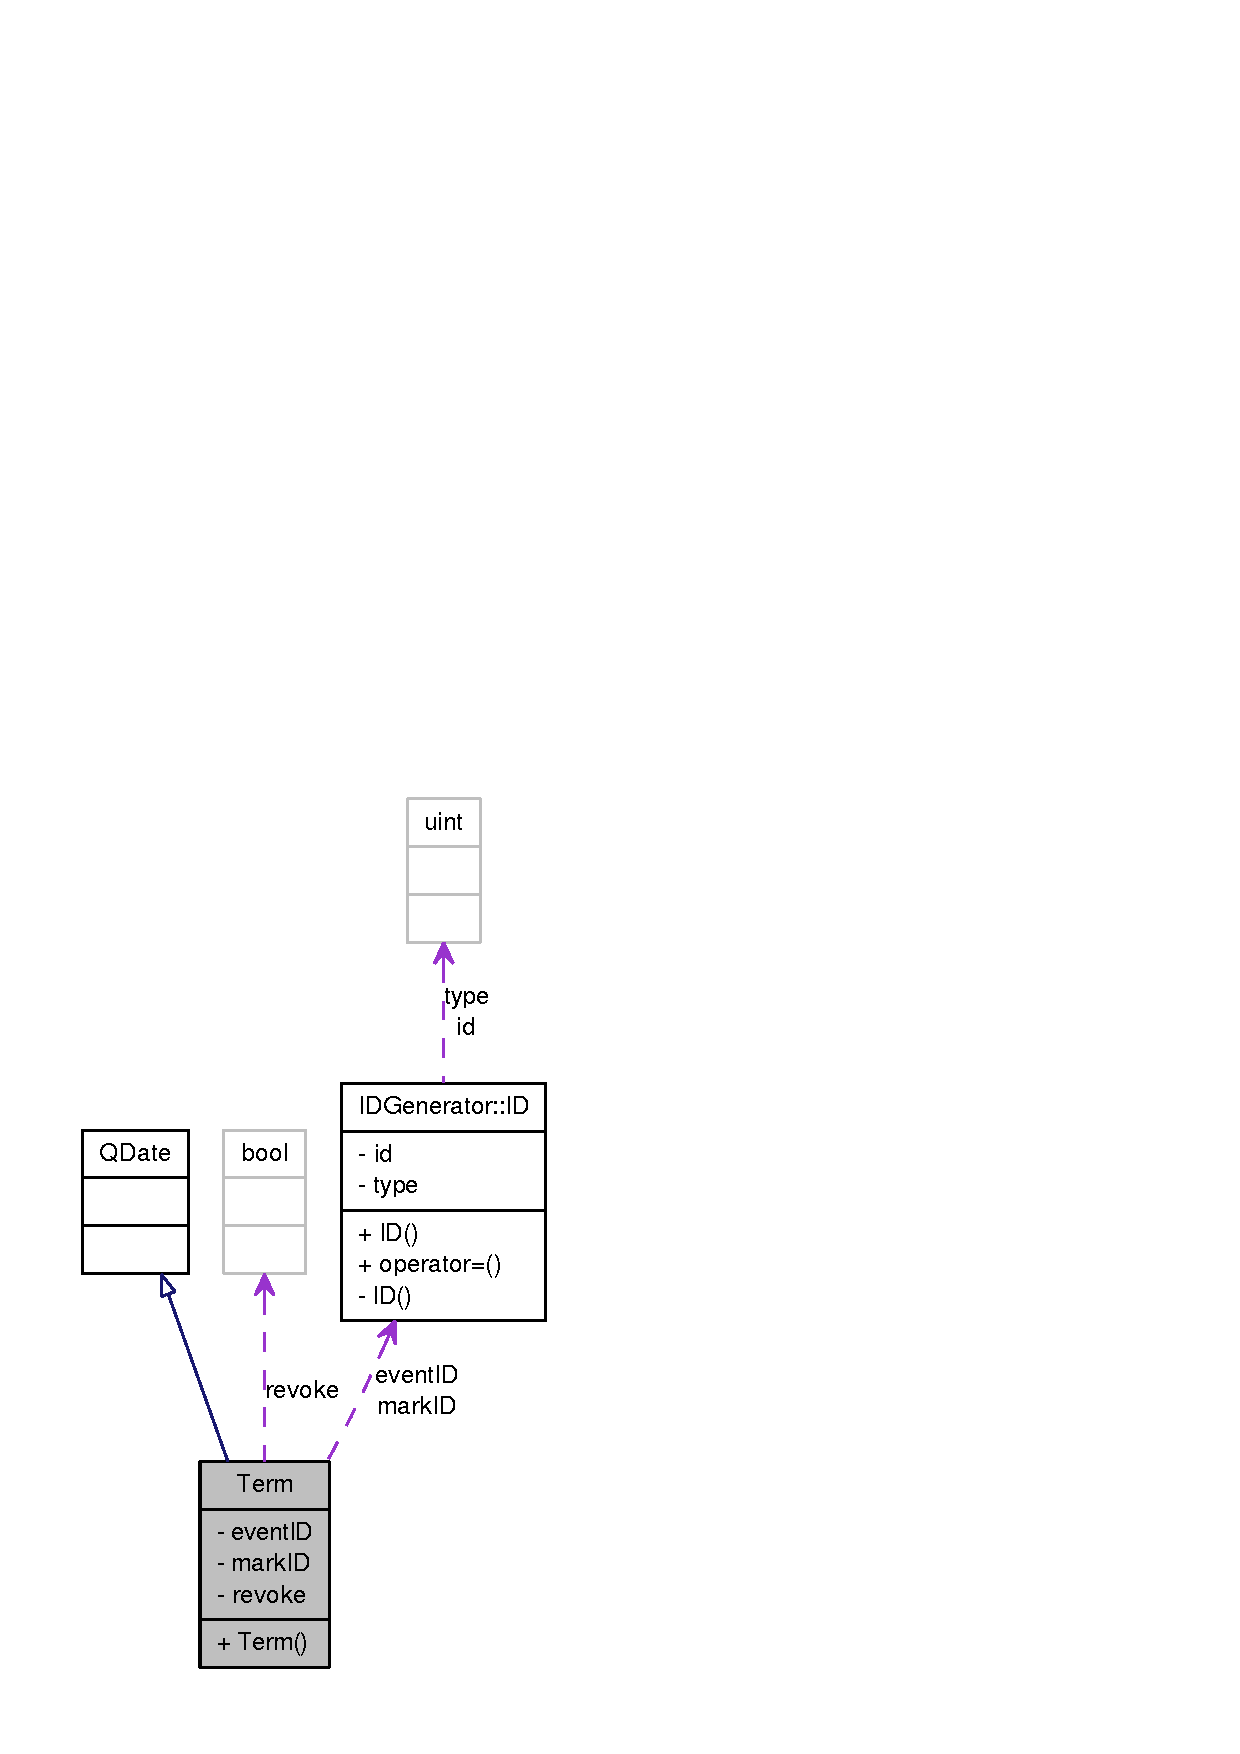
\includegraphics[height=400pt]{classTerm__coll__graph}
\end{center}
\end{figure}
\subsection*{Metody publiczne}
\begin{DoxyCompactItemize}
\item 
\hyperlink{classTerm_a8621decf6499e1b597de930add62240a}{Term} (\hyperlink{classIDGenerator_1_1ID}{IDGenerator::ID} event)
\begin{DoxyCompactList}\small\item\em Inicjalizuje obiekt reprezentujący termin danego wydarzenia. \item\end{DoxyCompactList}\end{DoxyCompactItemize}
\subsection*{Atrybuty prywatne}
\begin{DoxyCompactItemize}
\item 
\hyperlink{classIDGenerator_1_1ID}{IDGenerator::ID} \hyperlink{classTerm_acc86c9d25865449a551947aa1597dec5}{eventID}
\begin{DoxyCompactList}\small\item\em Identyfikator wydarzenia. \item\end{DoxyCompactList}\item 
\hyperlink{classIDGenerator_1_1ID}{IDGenerator::ID} \hyperlink{classTerm_a59508892d24fb82de0db91a377c690fb}{markID}
\begin{DoxyCompactList}\small\item\em Identyfikator oceny -\/ skutku egzekucji wydarzenia. \item\end{DoxyCompactList}\item 
bool \hyperlink{classTerm_a58a815dca7217ba0e9e4e084d7c91648}{revoke}
\begin{DoxyCompactList}\small\item\em Czy jest odwołany. \item\end{DoxyCompactList}\end{DoxyCompactItemize}
\subsection*{Przyjaciele}
\begin{DoxyCompactItemize}
\item 
QDataStream \& \hyperlink{classTerm_a607138da9b016f91528f99ab09407712}{operator$<$$<$} (QDataStream \&stream, const \hyperlink{classTerm}{Term} \&term)
\begin{DoxyCompactList}\small\item\em Zapisuje dany termin do danego strumienia. \item\end{DoxyCompactList}\item 
QDataStream \& \hyperlink{classTerm_ad3ecfcfe45e8df9b765a1b06be05a457}{operator$>$$>$} (QDataStream \&stream, \hyperlink{classTerm}{Term} \&term)
\begin{DoxyCompactList}\small\item\em Odczytuje dany termin z danego strumienia. \item\end{DoxyCompactList}\end{DoxyCompactItemize}


\subsection{Opis szczegółowy}
Reprezentacja egzekucji wydarzenia. Jest również odnośnikiem do danego wydarzenia. 

Definicja w linii 9 pliku term.h.



\subsection{Dokumentacja konstruktora i destruktora}
\hypertarget{classTerm_a8621decf6499e1b597de930add62240a}{
\index{Term@{Term}!Term@{Term}}
\index{Term@{Term}!Term@{Term}}
\subsubsection[{Term}]{\setlength{\rightskip}{0pt plus 5cm}Term::Term ({\bf IDGenerator::ID} {\em event})\hspace{0.3cm}{\ttfamily  \mbox{[}inline\mbox{]}}}}
\label{classTerm_a8621decf6499e1b597de930add62240a}


Inicjalizuje obiekt reprezentujący termin danego wydarzenia. 


\begin{DoxyParams}{Parametry}
\item[{\em event}]Identyfikator wydarzenia związanego z tym terminem \end{DoxyParams}


Definicja w linii 29 pliku term.h.




\begin{DoxyCode}
29 : eventID(event) {}
\end{DoxyCode}




\subsection{Dokumentacja przyjaciół i funkcji związanych}
\hypertarget{classTerm_a607138da9b016f91528f99ab09407712}{
\index{Term@{Term}!operator$<$$<$@{operator$<$$<$}}
\index{operator$<$$<$@{operator$<$$<$}!Term@{Term}}
\subsubsection[{operator$<$$<$}]{\setlength{\rightskip}{0pt plus 5cm}QDataStream\& operator$<$$<$ (QDataStream \& {\em stream}, \/  const {\bf Term} \& {\em term})\hspace{0.3cm}{\ttfamily  \mbox{[}friend\mbox{]}}}}
\label{classTerm_a607138da9b016f91528f99ab09407712}


Zapisuje dany termin do danego strumienia. 


\begin{DoxyParams}{Parametry}
\item[{\em stream}]Strumień do którego będzie zapisany termin. \item[{\em term}]Termin który zostanie zapisany. \end{DoxyParams}
\begin{DoxyReturn}{Zwraca}
Ten sam strumień. 
\end{DoxyReturn}


Definicja w linii 3 pliku term.cpp.




\begin{DoxyCode}
4 {
5     const QDate &date=term;
6     return stream<<date<<term.eventID<<term.markID;
7 }
\end{DoxyCode}


\hypertarget{classTerm_ad3ecfcfe45e8df9b765a1b06be05a457}{
\index{Term@{Term}!operator$>$$>$@{operator$>$$>$}}
\index{operator$>$$>$@{operator$>$$>$}!Term@{Term}}
\subsubsection[{operator$>$$>$}]{\setlength{\rightskip}{0pt plus 5cm}QDataStream\& operator$>$$>$ (QDataStream \& {\em stream}, \/  {\bf Term} \& {\em term})\hspace{0.3cm}{\ttfamily  \mbox{[}friend\mbox{]}}}}
\label{classTerm_ad3ecfcfe45e8df9b765a1b06be05a457}


Odczytuje dany termin z danego strumienia. 


\begin{DoxyParams}{Parametry}
\item[{\em stream}]Strumień z którego będzie odczytany termin. \item[{\em term}]Termin który zostanie zainicjalizowany odczytanymi danymi. \end{DoxyParams}
\begin{DoxyReturn}{Zwraca}
Ten sam strumień. 
\end{DoxyReturn}


Definicja w linii 9 pliku term.cpp.




\begin{DoxyCode}
10 {
11     QDate &date=term;
12     return stream>>date>>term.eventID>>term.markID;
13 }
\end{DoxyCode}




\subsection{Dokumentacja atrybutów składowych}
\hypertarget{classTerm_acc86c9d25865449a551947aa1597dec5}{
\index{Term@{Term}!eventID@{eventID}}
\index{eventID@{eventID}!Term@{Term}}
\subsubsection[{eventID}]{\setlength{\rightskip}{0pt plus 5cm}{\bf IDGenerator::ID} {\bf Term::eventID}\hspace{0.3cm}{\ttfamily  \mbox{[}private\mbox{]}}}}
\label{classTerm_acc86c9d25865449a551947aa1597dec5}


Identyfikator wydarzenia. 



Definicja w linii 31 pliku term.h.



Odwołania w operator$<$$<$() i operator$>$$>$().

\hypertarget{classTerm_a59508892d24fb82de0db91a377c690fb}{
\index{Term@{Term}!markID@{markID}}
\index{markID@{markID}!Term@{Term}}
\subsubsection[{markID}]{\setlength{\rightskip}{0pt plus 5cm}{\bf IDGenerator::ID} {\bf Term::markID}\hspace{0.3cm}{\ttfamily  \mbox{[}private\mbox{]}}}}
\label{classTerm_a59508892d24fb82de0db91a377c690fb}


Identyfikator oceny -\/ skutku egzekucji wydarzenia. 



Definicja w linii 32 pliku term.h.



Odwołania w operator$<$$<$() i operator$>$$>$().

\hypertarget{classTerm_a58a815dca7217ba0e9e4e084d7c91648}{
\index{Term@{Term}!revoke@{revoke}}
\index{revoke@{revoke}!Term@{Term}}
\subsubsection[{revoke}]{\setlength{\rightskip}{0pt plus 5cm}bool {\bf Term::revoke}\hspace{0.3cm}{\ttfamily  \mbox{[}private\mbox{]}}}}
\label{classTerm_a58a815dca7217ba0e9e4e084d7c91648}


Czy jest odwołany. 



Definicja w linii 33 pliku term.h.



Dokumentacja dla tej klasy została wygenerowana z pliku:\begin{DoxyCompactItemize}
\item 
include/\hyperlink{term_8h}{term.h}\end{DoxyCompactItemize}

\hypertarget{classType}{
\section{Dokumentacja klasy Type}
\label{classType}\index{Type@{Type}}
}


{\ttfamily \#include $<$type.h$>$}



Diagram współpracy dla Type:\nopagebreak
\begin{figure}[H]
\begin{center}
\leavevmode
\includegraphics[width=156pt]{classType__coll__graph}
\end{center}
\end{figure}
\subsection*{Atrybuty prywatne}
\begin{DoxyCompactItemize}
\item 
bool \hyperlink{classType_a443615a82c231e8d640b1b44e53d64b4}{exist}
\begin{DoxyCompactList}\small\item\em Czy ten obiekt reprezentuje dane. \item\end{DoxyCompactList}\item 
QString \hyperlink{classType_a6e24434e904a6dfd418c73f160460bac}{name}
\begin{DoxyCompactList}\small\item\em Nazwa typu. \item\end{DoxyCompactList}\end{DoxyCompactItemize}


\subsection{Opis szczegółowy}


Definicja w linii 6 pliku type.h.



\subsection{Dokumentacja atrybutów składowych}
\hypertarget{classType_a443615a82c231e8d640b1b44e53d64b4}{
\index{Type@{Type}!exist@{exist}}
\index{exist@{exist}!Type@{Type}}
\subsubsection[{exist}]{\setlength{\rightskip}{0pt plus 5cm}bool {\bf Type::exist}\hspace{0.3cm}{\ttfamily  \mbox{[}private\mbox{]}}}}
\label{classType_a443615a82c231e8d640b1b44e53d64b4}


Czy ten obiekt reprezentuje dane. 



Definicja w linii 10 pliku type.h.

\hypertarget{classType_a6e24434e904a6dfd418c73f160460bac}{
\index{Type@{Type}!name@{name}}
\index{name@{name}!Type@{Type}}
\subsubsection[{name}]{\setlength{\rightskip}{0pt plus 5cm}QString {\bf Type::name}\hspace{0.3cm}{\ttfamily  \mbox{[}private\mbox{]}}}}
\label{classType_a6e24434e904a6dfd418c73f160460bac}


Nazwa typu. 



Definicja w linii 11 pliku type.h.



Dokumentacja dla tej klasy została wygenerowana z pliku:\begin{DoxyCompactItemize}
\item 
include/\hyperlink{type_8h}{type.h}\end{DoxyCompactItemize}

\hypertarget{classobsolete_1_1TypeID}{
\section{Dokumentacja klasy obsolete::TypeID}
\label{classobsolete_1_1TypeID}\index{obsolete::TypeID@{obsolete::TypeID}}
}


Klasa reprezentująca identyfikator typu wydarzenia.  




{\ttfamily \#include $<$typeid.h$>$}



Diagram dziedziczenia dla obsolete::TypeID\nopagebreak
\begin{figure}[H]
\begin{center}
\leavevmode
\includegraphics[height=400pt]{classobsolete_1_1TypeID__inherit__graph}
\end{center}
\end{figure}


Diagram współpracy dla obsolete::TypeID:\nopagebreak
\begin{figure}[H]
\begin{center}
\leavevmode
\includegraphics[height=400pt]{classobsolete_1_1TypeID__coll__graph}
\end{center}
\end{figure}
\subsection*{Statyczne metody publiczne}
\begin{DoxyCompactItemize}
\item 
static \hyperlink{classobsolete_1_1AbstractReservedID}{AbstractReservedID} \hyperlink{classobsolete_1_1AbstractReservedID_a38fa00bf6097ab9cff285c8480c8097e}{createID} (uint \hyperlink{classobsolete_1_1ID}{ID})
\begin{DoxyCompactList}\small\item\em Opakowuje numer porządkowy zadaną liczbą. \item\end{DoxyCompactList}\end{DoxyCompactItemize}
\subsection*{Atrybuty chronione}
\begin{DoxyCompactItemize}
\item 
uint \hyperlink{classobsolete_1_1AbstractID_a5f67fa1c7d96085f0ef41193b60b570c}{ID}
\begin{DoxyCompactList}\small\item\em Reprezentowany \hyperlink{classobsolete_1_1ID}{ID}. \item\end{DoxyCompactList}\end{DoxyCompactItemize}


\subsection{Opis szczegółowy}
Klasa reprezentująca identyfikator typu wydarzenia. 

Definicja w linii 10 pliku typeid.h.



\subsection{Dokumentacja funkcji składowych}
\hypertarget{classobsolete_1_1AbstractReservedID_a38fa00bf6097ab9cff285c8480c8097e}{
\index{obsolete::TypeID@{obsolete::TypeID}!createID@{createID}}
\index{createID@{createID}!obsolete::TypeID@{obsolete::TypeID}}
\subsubsection[{createID}]{\setlength{\rightskip}{0pt plus 5cm}static {\bf AbstractReservedID} obsolete::AbstractReservedID::createID (uint {\em ID})\hspace{0.3cm}{\ttfamily  \mbox{[}inline, static, inherited\mbox{]}}}}
\label{classobsolete_1_1AbstractReservedID_a38fa00bf6097ab9cff285c8480c8097e}


Opakowuje numer porządkowy zadaną liczbą. 



\subsection{Dokumentacja atrybutów składowych}
\hypertarget{classobsolete_1_1AbstractID_a5f67fa1c7d96085f0ef41193b60b570c}{
\index{obsolete::TypeID@{obsolete::TypeID}!ID@{ID}}
\index{ID@{ID}!obsolete::TypeID@{obsolete::TypeID}}
\subsubsection[{ID}]{\setlength{\rightskip}{0pt plus 5cm}uint {\bf obsolete::AbstractID::ID}\hspace{0.3cm}{\ttfamily  \mbox{[}protected, inherited\mbox{]}}}}
\label{classobsolete_1_1AbstractID_a5f67fa1c7d96085f0ef41193b60b570c}


Reprezentowany \hyperlink{classobsolete_1_1ID}{ID}. 



Definicja w linii 34 pliku abstractid.h.



Dokumentacja dla tej klasy została wygenerowana z pliku:\begin{DoxyCompactItemize}
\item 
include/obsolete/\hyperlink{typeid_8h}{typeid.h}\end{DoxyCompactItemize}

\hypertarget{classobsolete_1_1TypeIDGenerator}{
\section{Dokumentacja klasy obsolete::TypeIDGenerator}
\label{classobsolete_1_1TypeIDGenerator}\index{obsolete::TypeIDGenerator@{obsolete::TypeIDGenerator}}
}


Generator generatorów obiektów \hyperlink{classobsolete_1_1TypeID}{TypeID}.  




{\ttfamily \#include $<$typeidgenerator.h$>$}



Diagram dziedziczenia dla obsolete::TypeIDGenerator\nopagebreak
\begin{figure}[H]
\begin{center}
\leavevmode
\includegraphics[width=218pt]{classobsolete_1_1TypeIDGenerator__inherit__graph}
\end{center}
\end{figure}


Diagram współpracy dla obsolete::TypeIDGenerator:\nopagebreak
\begin{figure}[H]
\begin{center}
\leavevmode
\includegraphics[height=400pt]{classobsolete_1_1TypeIDGenerator__coll__graph}
\end{center}
\end{figure}
\subsection*{Metody publiczne}
\begin{DoxyCompactItemize}
\item 
virtual \hyperlink{classobsolete_1_1ID}{ID} \hyperlink{classobsolete_1_1AbstractIDGenerator_a39d2f0147e3a028fef8299770e23db90}{createID} ()
\begin{DoxyCompactList}\small\item\em Tworzy nowy identyfikator. \item\end{DoxyCompactList}\end{DoxyCompactItemize}
\subsection*{Statyczne metody publiczne}
\begin{DoxyCompactItemize}
\item 
static \hyperlink{classobsolete_1_1ID}{ID} \hyperlink{classobsolete_1_1AbstractIDGenerator_a330da88ba80820ca6ce0a29cbbab9e1b}{createVoidID} ()
\begin{DoxyCompactList}\small\item\em Tworzy niezainicjowany identyfikator. \item\end{DoxyCompactList}\end{DoxyCompactItemize}
\subsection*{Atrybuty chronione}
\begin{DoxyCompactItemize}
\item 
uint \hyperlink{classobsolete_1_1AbstractID_a5f67fa1c7d96085f0ef41193b60b570c}{ID}
\begin{DoxyCompactList}\small\item\em Reprezentowany \hyperlink{classobsolete_1_1ID}{ID}. \item\end{DoxyCompactList}\end{DoxyCompactItemize}


\subsection{Opis szczegółowy}
Generator generatorów obiektów \hyperlink{classobsolete_1_1TypeID}{TypeID}. 

Definicja w linii 10 pliku typeidgenerator.h.



\subsection{Dokumentacja funkcji składowych}
\hypertarget{classobsolete_1_1AbstractIDGenerator_a39d2f0147e3a028fef8299770e23db90}{
\index{obsolete::TypeIDGenerator@{obsolete::TypeIDGenerator}!createID@{createID}}
\index{createID@{createID}!obsolete::TypeIDGenerator@{obsolete::TypeIDGenerator}}
\subsubsection[{createID}]{\setlength{\rightskip}{0pt plus 5cm}virtual {\bf ID} obsolete::AbstractIDGenerator::createID ()\hspace{0.3cm}{\ttfamily  \mbox{[}virtual, inherited\mbox{]}}}}
\label{classobsolete_1_1AbstractIDGenerator_a39d2f0147e3a028fef8299770e23db90}


Tworzy nowy identyfikator. 

\hypertarget{classobsolete_1_1AbstractIDGenerator_a330da88ba80820ca6ce0a29cbbab9e1b}{
\index{obsolete::TypeIDGenerator@{obsolete::TypeIDGenerator}!createVoidID@{createVoidID}}
\index{createVoidID@{createVoidID}!obsolete::TypeIDGenerator@{obsolete::TypeIDGenerator}}
\subsubsection[{createVoidID}]{\setlength{\rightskip}{0pt plus 5cm}static {\bf ID} obsolete::AbstractIDGenerator::createVoidID ()\hspace{0.3cm}{\ttfamily  \mbox{[}static, inherited\mbox{]}}}}
\label{classobsolete_1_1AbstractIDGenerator_a330da88ba80820ca6ce0a29cbbab9e1b}


Tworzy niezainicjowany identyfikator. 



\subsection{Dokumentacja atrybutów składowych}
\hypertarget{classobsolete_1_1AbstractID_a5f67fa1c7d96085f0ef41193b60b570c}{
\index{obsolete::TypeIDGenerator@{obsolete::TypeIDGenerator}!ID@{ID}}
\index{ID@{ID}!obsolete::TypeIDGenerator@{obsolete::TypeIDGenerator}}
\subsubsection[{ID}]{\setlength{\rightskip}{0pt plus 5cm}uint {\bf obsolete::AbstractID::ID}\hspace{0.3cm}{\ttfamily  \mbox{[}protected, inherited\mbox{]}}}}
\label{classobsolete_1_1AbstractID_a5f67fa1c7d96085f0ef41193b60b570c}


Reprezentowany \hyperlink{classobsolete_1_1ID}{ID}. 



Definicja w linii 34 pliku abstractid.h.



Dokumentacja dla tej klasy została wygenerowana z pliku:\begin{DoxyCompactItemize}
\item 
include/obsolete/\hyperlink{typeidgenerator_8h}{typeidgenerator.h}\end{DoxyCompactItemize}

\chapter{Dokumentacja plików}
\hypertarget{CMakeCCompilerId_8c}{
\section{Dokumentacja pliku build/CMakeFiles/CompilerIdC/CMakeCCompilerId.c}
\label{CMakeCCompilerId_8c}\index{build/CMakeFiles/CompilerIdC/CMakeCCompilerId.c@{build/CMakeFiles/CompilerIdC/CMakeCCompilerId.c}}
}
\subsection*{Definicje}
\begin{DoxyCompactItemize}
\item 
\#define \hyperlink{CMakeCCompilerId_8c_a81dee0709ded976b2e0319239f72d174}{COMPILER\_\-ID}~\char`\"{}\char`\"{}
\item 
\#define \hyperlink{CMakeCCompilerId_8c_adbc5372f40838899018fadbc89bd588b}{PLATFORM\_\-ID}~\char`\"{}\char`\"{}
\item 
\#define \hyperlink{CMakeCCompilerId_8c_aba35d0d200deaeb06aee95ca297acb28}{ARCHITECTURE\_\-ID}~\char`\"{}\char`\"{}
\end{DoxyCompactItemize}
\subsection*{Funkcje}
\begin{DoxyCompactItemize}
\item 
int \hyperlink{CMakeCCompilerId_8c_a0ddf1224851353fc92bfbff6f499fa97}{main} (int argc, char $\ast$argv\mbox{[}$\,$\mbox{]})
\end{DoxyCompactItemize}
\subsection*{Zmienne}
\begin{DoxyCompactItemize}
\item 
char $\ast$ \hyperlink{CMakeCCompilerId_8c_aab4f0400f2b990cc0cfaa596066ed23a}{info\_\-compiler} = \char`\"{}INFO\char`\"{} \char`\"{}:\char`\"{} \char`\"{}compiler\mbox{[}\char`\"{} \char`\"{}\char`\"{} \char`\"{}\mbox{]}\char`\"{}
\item 
char $\ast$ \hyperlink{CMakeCCompilerId_8c_abfa30dab5bd89c85774e2aaaca5262d1}{info\_\-platform} = \char`\"{}INFO\char`\"{} \char`\"{}:\char`\"{} \char`\"{}platform\mbox{[}\char`\"{} \char`\"{}\char`\"{} \char`\"{}\mbox{]}\char`\"{}
\item 
char $\ast$ \hyperlink{CMakeCCompilerId_8c_a12b947909f56ca28de40d457cc7f7513}{info\_\-arch} = \char`\"{}INFO\char`\"{} \char`\"{}:\char`\"{} \char`\"{}arch\mbox{[}\char`\"{} \char`\"{}\char`\"{} \char`\"{}\mbox{]}\char`\"{}
\end{DoxyCompactItemize}


\subsection{Dokumentacja definicji}
\hypertarget{CMakeCCompilerId_8c_aba35d0d200deaeb06aee95ca297acb28}{
\index{CMakeCCompilerId.c@{CMakeCCompilerId.c}!ARCHITECTURE\_\-ID@{ARCHITECTURE\_\-ID}}
\index{ARCHITECTURE\_\-ID@{ARCHITECTURE\_\-ID}!CMakeCCompilerId.c@{CMakeCCompilerId.c}}
\subsubsection[{ARCHITECTURE\_\-ID}]{\setlength{\rightskip}{0pt plus 5cm}\#define ARCHITECTURE\_\-ID~\char`\"{}\char`\"{}}}
\label{CMakeCCompilerId_8c_aba35d0d200deaeb06aee95ca297acb28}


Definicja w linii 191 pliku CMakeCCompilerId.c.

\hypertarget{CMakeCCompilerId_8c_a81dee0709ded976b2e0319239f72d174}{
\index{CMakeCCompilerId.c@{CMakeCCompilerId.c}!COMPILER\_\-ID@{COMPILER\_\-ID}}
\index{COMPILER\_\-ID@{COMPILER\_\-ID}!CMakeCCompilerId.c@{CMakeCCompilerId.c}}
\subsubsection[{COMPILER\_\-ID}]{\setlength{\rightskip}{0pt plus 5cm}\#define COMPILER\_\-ID~\char`\"{}\char`\"{}}}
\label{CMakeCCompilerId_8c_a81dee0709ded976b2e0319239f72d174}


Definicja w linii 77 pliku CMakeCCompilerId.c.

\hypertarget{CMakeCCompilerId_8c_adbc5372f40838899018fadbc89bd588b}{
\index{CMakeCCompilerId.c@{CMakeCCompilerId.c}!PLATFORM\_\-ID@{PLATFORM\_\-ID}}
\index{PLATFORM\_\-ID@{PLATFORM\_\-ID}!CMakeCCompilerId.c@{CMakeCCompilerId.c}}
\subsubsection[{PLATFORM\_\-ID}]{\setlength{\rightskip}{0pt plus 5cm}\#define PLATFORM\_\-ID~\char`\"{}\char`\"{}}}
\label{CMakeCCompilerId_8c_adbc5372f40838899018fadbc89bd588b}


Definicja w linii 167 pliku CMakeCCompilerId.c.



\subsection{Dokumentacja funkcji}
\hypertarget{CMakeCCompilerId_8c_a0ddf1224851353fc92bfbff6f499fa97}{
\index{CMakeCCompilerId.c@{CMakeCCompilerId.c}!main@{main}}
\index{main@{main}!CMakeCCompilerId.c@{CMakeCCompilerId.c}}
\subsubsection[{main}]{\setlength{\rightskip}{0pt plus 5cm}int main (int {\em argc}, \/  char $\ast$ {\em argv}\mbox{[}$\,$\mbox{]})}}
\label{CMakeCCompilerId_8c_a0ddf1224851353fc92bfbff6f499fa97}


Definicja w linii 208 pliku CMakeCCompilerId.c.



Odwołuje się do info\_\-arch, info\_\-compiler i info\_\-platform.




\begin{DoxyCode}
209 {
210   int require = 0;
211   require += info_compiler[argc];
212   require += info_platform[argc];
213   require += info_arch[argc];
214   (void)argv;
215   return require;
216 }
\end{DoxyCode}




\subsection{Dokumentacja zmiennych}
\hypertarget{CMakeCCompilerId_8c_a12b947909f56ca28de40d457cc7f7513}{
\index{CMakeCCompilerId.c@{CMakeCCompilerId.c}!info\_\-arch@{info\_\-arch}}
\index{info\_\-arch@{info\_\-arch}!CMakeCCompilerId.c@{CMakeCCompilerId.c}}
\subsubsection[{info\_\-arch}]{\setlength{\rightskip}{0pt plus 5cm}char$\ast$ {\bf info\_\-arch} = \char`\"{}INFO\char`\"{} \char`\"{}:\char`\"{} \char`\"{}arch\mbox{[}\char`\"{} \char`\"{}\char`\"{} \char`\"{}\mbox{]}\char`\"{}}}
\label{CMakeCCompilerId_8c_a12b947909f56ca28de40d457cc7f7513}


Definicja w linii 199 pliku CMakeCCompilerId.c.



Odwołania w main().

\hypertarget{CMakeCCompilerId_8c_aab4f0400f2b990cc0cfaa596066ed23a}{
\index{CMakeCCompilerId.c@{CMakeCCompilerId.c}!info\_\-compiler@{info\_\-compiler}}
\index{info\_\-compiler@{info\_\-compiler}!CMakeCCompilerId.c@{CMakeCCompilerId.c}}
\subsubsection[{info\_\-compiler}]{\setlength{\rightskip}{0pt plus 5cm}char$\ast$ {\bf info\_\-compiler} = \char`\"{}INFO\char`\"{} \char`\"{}:\char`\"{} \char`\"{}compiler\mbox{[}\char`\"{} \char`\"{}\char`\"{} \char`\"{}\mbox{]}\char`\"{}}}
\label{CMakeCCompilerId_8c_aab4f0400f2b990cc0cfaa596066ed23a}


Definicja w linii 85 pliku CMakeCCompilerId.c.



Odwołania w main().

\hypertarget{CMakeCCompilerId_8c_abfa30dab5bd89c85774e2aaaca5262d1}{
\index{CMakeCCompilerId.c@{CMakeCCompilerId.c}!info\_\-platform@{info\_\-platform}}
\index{info\_\-platform@{info\_\-platform}!CMakeCCompilerId.c@{CMakeCCompilerId.c}}
\subsubsection[{info\_\-platform}]{\setlength{\rightskip}{0pt plus 5cm}char$\ast$ {\bf info\_\-platform} = \char`\"{}INFO\char`\"{} \char`\"{}:\char`\"{} \char`\"{}platform\mbox{[}\char`\"{} \char`\"{}\char`\"{} \char`\"{}\mbox{]}\char`\"{}}}
\label{CMakeCCompilerId_8c_abfa30dab5bd89c85774e2aaaca5262d1}


Definicja w linii 198 pliku CMakeCCompilerId.c.



Odwołania w main().


\include{CMakeCXXCompilerId_8cpp}
\hypertarget{event_8h}{
\section{Dokumentacja pliku include/event.h}
\label{event_8h}\index{include/event.h@{include/event.h}}
}
{\ttfamily \#include $<$QtCore/QList$>$}\par
{\ttfamily \#include $<$QtCore/QDataStream$>$}\par
{\ttfamily \#include \char`\"{}term.h\char`\"{}}\par
{\ttfamily \#include $<$QDate$>$}\par
{\ttfamily \#include $<$QtCore/QtGlobal$>$}\par
{\ttfamily \#include \char`\"{}idgenerator.h\char`\"{}}\par
Wykres zależności załączania dla event.h:\nopagebreak
\begin{figure}[H]
\begin{center}
\leavevmode
\includegraphics[width=191pt]{event_8h__incl}
\end{center}
\end{figure}
Ten wykres pokazuje, które pliki bezpośrednio lub pośrednio załączają ten plik:\nopagebreak
\begin{figure}[H]
\begin{center}
\leavevmode
\includegraphics[width=77pt]{event_8h__dep__incl}
\end{center}
\end{figure}
\subsection*{Komponenty}
\begin{DoxyCompactItemize}
\item 
class \hyperlink{classEvent}{Event}
\begin{DoxyCompactList}\small\item\em Reprezentuje zdarzenie w postaci zdefiniowanej przez użytkownika. \item\end{DoxyCompactList}\end{DoxyCompactItemize}
\subsection*{Funkcje}
\begin{DoxyCompactItemize}
\item 
QDataStream \& \hyperlink{event_8h_a62e8730ab4dc16e3d456b527a12635b3}{operator$<$$<$} (QDataStream \&stream, const \hyperlink{classEvent}{Event} \&event)
\begin{DoxyCompactList}\small\item\em Zapisuje informacje o danym wydarzeniu do danego strumienia. \item\end{DoxyCompactList}\item 
QDataStream \& \hyperlink{event_8h_a055427e98ad131966edb6fb652add004}{operator$>$$>$} (QDataStream \&stream, \hyperlink{classEvent}{Event} \&event)
\begin{DoxyCompactList}\small\item\em Odczytuje informacje o danym wydarzeniu z danego strumienia. \item\end{DoxyCompactList}\end{DoxyCompactItemize}


\subsection{Dokumentacja funkcji}
\hypertarget{event_8h_a62e8730ab4dc16e3d456b527a12635b3}{
\index{event.h@{event.h}!operator$<$$<$@{operator$<$$<$}}
\index{operator$<$$<$@{operator$<$$<$}!event.h@{event.h}}
\subsubsection[{operator$<$$<$}]{\setlength{\rightskip}{0pt plus 5cm}QDataStream\& operator$<$$<$ (QDataStream \& {\em stream}, \/  const {\bf Event} \& {\em event})}}
\label{event_8h_a62e8730ab4dc16e3d456b527a12635b3}


Zapisuje informacje o danym wydarzeniu do danego strumienia. 


\begin{DoxyParams}{Parametry}
\item[{\em stream}]Strumień do którego będą zapisywane dane. \item[{\em event}]Wydarzenie które będzie zapisywane. \end{DoxyParams}
\begin{DoxyReturn}{Zwraca}
Ten sam strumień. 
\end{DoxyReturn}


Definicja w linii 3 pliku event.cpp.




\begin{DoxyCode}
4 {
5     return stream<<event.subjectID<<event.typeID<<event.terms;
6 }
\end{DoxyCode}


\hypertarget{event_8h_a055427e98ad131966edb6fb652add004}{
\index{event.h@{event.h}!operator$>$$>$@{operator$>$$>$}}
\index{operator$>$$>$@{operator$>$$>$}!event.h@{event.h}}
\subsubsection[{operator$>$$>$}]{\setlength{\rightskip}{0pt plus 5cm}QDataStream\& operator$>$$>$ (QDataStream \& {\em stream}, \/  {\bf Event} \& {\em event})}}
\label{event_8h_a055427e98ad131966edb6fb652add004}


Odczytuje informacje o danym wydarzeniu z danego strumienia. 


\begin{DoxyParams}{Parametry}
\item[{\em stream}]Strumień z którego będą odczytywane dane. \item[{\em event}]Wydarzenie które zostanie zainicjalizowane wczytanymi danymi. \end{DoxyParams}
\begin{DoxyReturn}{Zwraca}
Ten sam strumień. 
\end{DoxyReturn}


Definicja w linii 8 pliku event.cpp.




\begin{DoxyCode}
9 {
10     return stream>>event.subjectID<<event.typeID<<event.terms;
11 }
\end{DoxyCode}



\hypertarget{events_8h}{
\section{Dokumentacja pliku include/events.h}
\label{events_8h}\index{include/events.h@{include/events.h}}
}
{\ttfamily \#include $<$QtCore/QList$>$}\par
{\ttfamily \#include $<$QtCore/QFile$>$}\par
{\ttfamily \#include \char`\"{}event.h\char`\"{}}\par
{\ttfamily \#include $<$QtCore/QDataStream$>$}\par
{\ttfamily \#include \char`\"{}term.h\char`\"{}}\par
{\ttfamily \#include \char`\"{}generatoridgenerator.h\char`\"{}}\par
Wykres zależności załączania dla events.h:\nopagebreak
\begin{figure}[H]
\begin{center}
\leavevmode
\includegraphics[width=245pt]{events_8h__incl}
\end{center}
\end{figure}
Ten wykres pokazuje, które pliki bezpośrednio lub pośrednio załączają ten plik:\nopagebreak
\begin{figure}[H]
\begin{center}
\leavevmode
\includegraphics[width=80pt]{events_8h__dep__incl}
\end{center}
\end{figure}
\subsection*{Komponenty}
\begin{DoxyCompactItemize}
\item 
class \hyperlink{classEvents}{Events}
\begin{DoxyCompactList}\small\item\em Klasa przechowuje wszystkie wydarzenia i zarządza nimi. \item\end{DoxyCompactList}\end{DoxyCompactItemize}
\subsection*{Funkcje}
\begin{DoxyCompactItemize}
\item 
QDataStream \& \hyperlink{events_8h_a560f3fdc9b76a9fe9146335122ecda39}{operator$<$$<$} (QDataStream \&stream, const \hyperlink{classEvents}{Events} \&events)
\begin{DoxyCompactList}\small\item\em Zapisuje informacje o wydarzeniach do danego strumienia. \item\end{DoxyCompactList}\item 
QDataStream \& \hyperlink{events_8h_a9e3a2b909c5dcbc9519365ccafc4a96f}{operator$>$$>$} (QDataStream \&stream, \hyperlink{classEvents}{Events} \&events)
\begin{DoxyCompactList}\small\item\em Odczytuje informacje o wydarzeniach z danego strumienia. \item\end{DoxyCompactList}\end{DoxyCompactItemize}


\subsection{Dokumentacja funkcji}
\hypertarget{events_8h_a560f3fdc9b76a9fe9146335122ecda39}{
\index{events.h@{events.h}!operator$<$$<$@{operator$<$$<$}}
\index{operator$<$$<$@{operator$<$$<$}!events.h@{events.h}}
\subsubsection[{operator$<$$<$}]{\setlength{\rightskip}{0pt plus 5cm}QDataStream\& operator$<$$<$ (QDataStream \& {\em stream}, \/  const {\bf Events} \& {\em events})}}
\label{events_8h_a560f3fdc9b76a9fe9146335122ecda39}


Zapisuje informacje o wydarzeniach do danego strumienia. 


\begin{DoxyParams}{Parametry}
\item[{\em stream}]Strumień do którego będą zapisywane dane. \item[{\em events}]Wydarzenia które będzie zapisywane. \end{DoxyParams}
\begin{DoxyReturn}{Zwraca}
Ten sam strumień. 
\end{DoxyReturn}


Definicja w linii 5 pliku events.cpp.



Odwołuje się do Events::eventIDGenerator i Events::events.




\begin{DoxyCode}
6 {
7     return stream<<events.eventIDGenerator<<events.events;
8 }
\end{DoxyCode}


\hypertarget{events_8h_a9e3a2b909c5dcbc9519365ccafc4a96f}{
\index{events.h@{events.h}!operator$>$$>$@{operator$>$$>$}}
\index{operator$>$$>$@{operator$>$$>$}!events.h@{events.h}}
\subsubsection[{operator$>$$>$}]{\setlength{\rightskip}{0pt plus 5cm}QDataStream\& operator$>$$>$ (QDataStream \& {\em stream}, \/  {\bf Events} \& {\em events})}}
\label{events_8h_a9e3a2b909c5dcbc9519365ccafc4a96f}


Odczytuje informacje o wydarzeniach z danego strumienia. 


\begin{DoxyParams}{Parametry}
\item[{\em stream}]Strumień z którego będą odczytywane dane. \item[{\em events}]Obiekt klasy \hyperlink{classEvents}{Events} który zostanie zainicjalizowany wczytanymi danymi. \end{DoxyParams}
\begin{DoxyReturn}{Zwraca}
Ten sam strumień. 
\end{DoxyReturn}


Definicja w linii 10 pliku events.cpp.



Odwołuje się do Events::eventIDGenerator i Events::events.




\begin{DoxyCode}
11 {
12     return stream>>events.eventIDGenerator>>events.events;
13 }
\end{DoxyCode}



\hypertarget{generatoridgenerator_8h}{
\section{Dokumentacja pliku include/generatoridgenerator.h}
\label{generatoridgenerator_8h}\index{include/generatoridgenerator.h@{include/generatoridgenerator.h}}
}
{\ttfamily \#include \char`\"{}idgenerator.h\char`\"{}}\par
Wykres zależności załączania dla generatoridgenerator.h:\nopagebreak
\begin{figure}[H]
\begin{center}
\leavevmode
\includegraphics[width=148pt]{generatoridgenerator_8h__incl}
\end{center}
\end{figure}
Ten wykres pokazuje, które pliki bezpośrednio lub pośrednio załączają ten plik:\nopagebreak
\begin{figure}[H]
\begin{center}
\leavevmode
\includegraphics[width=420pt]{generatoridgenerator_8h__dep__incl}
\end{center}
\end{figure}
\subsection*{Komponenty}
\begin{DoxyCompactItemize}
\item 
class \hyperlink{classGeneratorIDGenerator}{GeneratorIDGenerator}
\begin{DoxyCompactList}\small\item\em Ta klasa odpowiada za generowanie generatorów identyfikatorów. \item\end{DoxyCompactList}\end{DoxyCompactItemize}

\hypertarget{idgenerator_8h}{
\section{Dokumentacja pliku include/idgenerator.h}
\label{idgenerator_8h}\index{include/idgenerator.h@{include/idgenerator.h}}
}
{\ttfamily \#include $<$QtCore/QtGlobal$>$}\par
{\ttfamily \#include $<$QtCore/QDataStream$>$}\par
Wykres zależności załączania dla idgenerator.h:\nopagebreak
\begin{figure}[H]
\begin{center}
\leavevmode
\includegraphics[width=148pt]{idgenerator_8h__incl}
\end{center}
\end{figure}
Ten wykres pokazuje, które pliki bezpośrednio lub pośrednio załączają ten plik:\nopagebreak
\begin{figure}[H]
\begin{center}
\leavevmode
\includegraphics[width=420pt]{idgenerator_8h__dep__incl}
\end{center}
\end{figure}
\subsection*{Komponenty}
\begin{DoxyCompactItemize}
\item 
class \hyperlink{classIDGenerator}{IDGenerator}
\begin{DoxyCompactList}\small\item\em Generator identyfikatorów określonego typu. \item\end{DoxyCompactList}\item 
class \hyperlink{classIDGenerator_1_1ID}{IDGenerator::ID}
\begin{DoxyCompactList}\small\item\em Obiekt reprezentuje dany identyfikator określonego typu. \item\end{DoxyCompactList}\end{DoxyCompactItemize}
\subsection*{Funkcje}
\begin{DoxyCompactItemize}
\item 
QDataStream \& \hyperlink{idgenerator_8h_a4eb9e946c558bb876ce7b8fa462bfd5e}{operator$<$$<$} (QDataStream \&stream, const \hyperlink{classIDGenerator_1_1ID}{IDGenerator::ID} \&id)
\begin{DoxyCompactList}\small\item\em Zapisuje dany identyfikator do danego strumienia. \item\end{DoxyCompactList}\item 
QDataStream \& \hyperlink{idgenerator_8h_aeca67851b2c46cd46266ca668e8dc63c}{operator$>$$>$} (QDataStream \&stream, \hyperlink{classIDGenerator_1_1ID}{IDGenerator::ID} \&id)
\begin{DoxyCompactList}\small\item\em Odczytuje dany identyfikator z danego strumienia. \item\end{DoxyCompactList}\item 
QDataStream \& \hyperlink{idgenerator_8h_a244688be6d84ec73612ddd66ab376bd1}{operator$<$$<$} (QDataStream \&stream, const \hyperlink{classIDGenerator}{IDGenerator} \&generator)
\begin{DoxyCompactList}\small\item\em Zapisuje dany generator identyfikatorów do danego strumienia. \item\end{DoxyCompactList}\item 
QDataStream \& \hyperlink{idgenerator_8h_a4f86069b5b5ede60ff2e613fbcf10de4}{operator$>$$>$} (QDataStream \&stream, \hyperlink{classIDGenerator}{IDGenerator} \&generator)
\begin{DoxyCompactList}\small\item\em Odczytuje dany generator identyfikatorów z danego strumienia. \item\end{DoxyCompactList}\end{DoxyCompactItemize}


\subsection{Dokumentacja funkcji}
\hypertarget{idgenerator_8h_a244688be6d84ec73612ddd66ab376bd1}{
\index{idgenerator.h@{idgenerator.h}!operator$<$$<$@{operator$<$$<$}}
\index{operator$<$$<$@{operator$<$$<$}!idgenerator.h@{idgenerator.h}}
\subsubsection[{operator$<$$<$}]{\setlength{\rightskip}{0pt plus 5cm}QDataStream\& operator$<$$<$ (QDataStream \& {\em stream}, \/  const {\bf IDGenerator} \& {\em generator})}}
\label{idgenerator_8h_a244688be6d84ec73612ddd66ab376bd1}


Zapisuje dany generator identyfikatorów do danego strumienia. 


\begin{DoxyParams}{Parametry}
\item[{\em stream}]Strumień do którego będzie zapisany generator identyfikatorów. \item[{\em generator}]Generator identyfikatorów który zostanie zapisany. \end{DoxyParams}
\begin{DoxyReturn}{Zwraca}
Ten sam strumień. 
\end{DoxyReturn}


Definicja w linii 30 pliku idgenerator.cpp.



Odwołuje się do IDGenerator::freeID i IDGenerator::type.




\begin{DoxyCode}
31 {
32     return stream<<generator.type<<generator.freeID;
33 }
\end{DoxyCode}


\hypertarget{idgenerator_8h_a4eb9e946c558bb876ce7b8fa462bfd5e}{
\index{idgenerator.h@{idgenerator.h}!operator$<$$<$@{operator$<$$<$}}
\index{operator$<$$<$@{operator$<$$<$}!idgenerator.h@{idgenerator.h}}
\subsubsection[{operator$<$$<$}]{\setlength{\rightskip}{0pt plus 5cm}QDataStream\& operator$<$$<$ (QDataStream \& {\em stream}, \/  const {\bf IDGenerator::ID} \& {\em id})}}
\label{idgenerator_8h_a4eb9e946c558bb876ce7b8fa462bfd5e}


Zapisuje dany identyfikator do danego strumienia. 


\begin{DoxyParams}{Parametry}
\item[{\em stream}]Strumień do którego będzie zapisany identyfikator. \item[{\em id}]Identyfikator który zostanie zapisany. \end{DoxyParams}
\begin{DoxyReturn}{Zwraca}
Ten sam strumień. 
\end{DoxyReturn}


Definicja w linii 20 pliku idgenerator.cpp.




\begin{DoxyCode}
21 {
22     return stream<<id.type<<id.id;
23 }
\end{DoxyCode}


\hypertarget{idgenerator_8h_a4f86069b5b5ede60ff2e613fbcf10de4}{
\index{idgenerator.h@{idgenerator.h}!operator$>$$>$@{operator$>$$>$}}
\index{operator$>$$>$@{operator$>$$>$}!idgenerator.h@{idgenerator.h}}
\subsubsection[{operator$>$$>$}]{\setlength{\rightskip}{0pt plus 5cm}QDataStream\& operator$>$$>$ (QDataStream \& {\em stream}, \/  {\bf IDGenerator} \& {\em generator})}}
\label{idgenerator_8h_a4f86069b5b5ede60ff2e613fbcf10de4}


Odczytuje dany generator identyfikatorów z danego strumienia. 


\begin{DoxyParams}{Parametry}
\item[{\em stream}]Strumień z którego będzie odczytany generator identyfikatorów. \item[{\em generator}]Generator identyfikatorów który zostanie zainicjalizowany odczytanymi danymi. \end{DoxyParams}
\begin{DoxyReturn}{Zwraca}
Ten sam strumień. 
\end{DoxyReturn}


Definicja w linii 35 pliku idgenerator.cpp.



Odwołuje się do IDGenerator::freeID i IDGenerator::type.




\begin{DoxyCode}
36 {
37     return stream>>generator.type>>generator.freeID;
38 }
\end{DoxyCode}


\hypertarget{idgenerator_8h_aeca67851b2c46cd46266ca668e8dc63c}{
\index{idgenerator.h@{idgenerator.h}!operator$>$$>$@{operator$>$$>$}}
\index{operator$>$$>$@{operator$>$$>$}!idgenerator.h@{idgenerator.h}}
\subsubsection[{operator$>$$>$}]{\setlength{\rightskip}{0pt plus 5cm}QDataStream\& operator$>$$>$ (QDataStream \& {\em stream}, \/  {\bf IDGenerator::ID} \& {\em id})}}
\label{idgenerator_8h_aeca67851b2c46cd46266ca668e8dc63c}


Odczytuje dany identyfikator z danego strumienia. 


\begin{DoxyParams}{Parametry}
\item[{\em stream}]Strumień z którego będzie odczytany identyfikator. \item[{\em id}]Identyfikator który zostanie zainicjalizowany odczytanymi danymi. \end{DoxyParams}
\begin{DoxyReturn}{Zwraca}
Ten sam strumień. 
\end{DoxyReturn}


Definicja w linii 25 pliku idgenerator.cpp.




\begin{DoxyCode}
26 {
27     return stream>>id.type>>id.id;
28 }
\end{DoxyCode}



\hypertarget{abstractid_8h}{
\section{Dokumentacja pliku include/obsolete/abstractid.h}
\label{abstractid_8h}\index{include/obsolete/abstractid.h@{include/obsolete/abstractid.h}}
}
{\ttfamily \#include $<$QtCore/QtGlobal$>$}\par
{\ttfamily \#include $<$QtCore/QDataStream$>$}\par
Wykres zależności załączania dla abstractid.h:\nopagebreak
\begin{figure}[H]
\begin{center}
\leavevmode
\includegraphics[width=148pt]{abstractid_8h__incl}
\end{center}
\end{figure}
Ten wykres pokazuje, które pliki bezpośrednio lub pośrednio załączają ten plik:\nopagebreak
\begin{figure}[H]
\begin{center}
\leavevmode
\includegraphics[width=420pt]{abstractid_8h__dep__incl}
\end{center}
\end{figure}
\subsection*{Komponenty}
\begin{DoxyCompactItemize}
\item 
class \hyperlink{classobsolete_1_1AbstractID}{obsolete::AbstractID}
\begin{DoxyCompactList}\small\item\em Klasa bazowa dla wszystkich typów identyfikatorowych. \item\end{DoxyCompactList}\end{DoxyCompactItemize}
\subsection*{Przestrzenie nazw}
\begin{DoxyCompactItemize}
\item 
namespace \hyperlink{namespaceobsolete}{obsolete}
\end{DoxyCompactItemize}
\subsection*{Funkcje}
\begin{DoxyCompactItemize}
\item 
QDataStream \& \hyperlink{namespaceobsolete_ae67d47b6a22388897d176c4569da81d2}{obsolete::operator$<$$<$} (QDataStream \&stream, const AbstractID \&ID)
\begin{DoxyCompactList}\small\item\em Zapisuje dany identyfikator do danego strumienia. \item\end{DoxyCompactList}\item 
QDataStream \& \hyperlink{namespaceobsolete_aa4c713ba2a42ffbb45bbeca0e2800a76}{obsolete::operator$>$$>$} (QDataStream \&stream, AbstractID \&ID)
\begin{DoxyCompactList}\small\item\em Odczytuje dany identyfikator z danego strumienia. \item\end{DoxyCompactList}\end{DoxyCompactItemize}

\hypertarget{abstractidgenerator_8h}{
\section{Dokumentacja pliku include/obsolete/abstractidgenerator.h}
\label{abstractidgenerator_8h}\index{include/obsolete/abstractidgenerator.h@{include/obsolete/abstractidgenerator.h}}
}
{\ttfamily \#include \char`\"{}abstractid.h\char`\"{}}\par
{\ttfamily \#include $<$QtCore/QtGlobal$>$}\par
{\ttfamily \#include $<$QtCore/QDataStream$>$}\par
{\ttfamily \#include \char`\"{}abstractid.h\char`\"{}}\par
{\ttfamily \#include \char`\"{}abstractincrementalid.h\char`\"{}}\par
{\ttfamily \#include \char`\"{}abstractreservedid.h\char`\"{}}\par
Wykres zależności załączania dla abstractidgenerator.h:\nopagebreak
\begin{figure}[H]
\begin{center}
\leavevmode
\includegraphics[width=202pt]{abstractidgenerator_8h__incl}
\end{center}
\end{figure}
Ten wykres pokazuje, które pliki bezpośrednio lub pośrednio załączają ten plik:\nopagebreak
\begin{figure}[H]
\begin{center}
\leavevmode
\includegraphics[width=340pt]{abstractidgenerator_8h__dep__incl}
\end{center}
\end{figure}
\subsection*{Komponenty}
\begin{DoxyCompactItemize}
\item 
class \hyperlink{classobsolete_1_1AbstractIDGenerator}{obsolete::AbstractIDGenerator}
\begin{DoxyCompactList}\small\item\em Klasa bazowa obiektów-\/generatorów identyfikatorów. \item\end{DoxyCompactList}\end{DoxyCompactItemize}
\subsection*{Przestrzenie nazw}
\begin{DoxyCompactItemize}
\item 
namespace \hyperlink{namespaceobsolete}{obsolete}
\end{DoxyCompactItemize}

\hypertarget{abstractincrementalid_8h}{
\section{Dokumentacja pliku include/obsolete/abstractincrementalid.h}
\label{abstractincrementalid_8h}\index{include/obsolete/abstractincrementalid.h@{include/obsolete/abstractincrementalid.h}}
}
{\ttfamily \#include \char`\"{}abstractid.h\char`\"{}}\par
Wykres zależności załączania dla abstractincrementalid.h:\nopagebreak
\begin{figure}[H]
\begin{center}
\leavevmode
\includegraphics[width=148pt]{abstractincrementalid_8h__incl}
\end{center}
\end{figure}
Ten wykres pokazuje, które pliki bezpośrednio lub pośrednio załączają ten plik:\nopagebreak
\begin{figure}[H]
\begin{center}
\leavevmode
\includegraphics[width=420pt]{abstractincrementalid_8h__dep__incl}
\end{center}
\end{figure}
\subsection*{Komponenty}
\begin{DoxyCompactItemize}
\item 
class \hyperlink{classobsolete_1_1AbstractIncrementalID}{obsolete::AbstractIncrementalID}
\begin{DoxyCompactList}\small\item\em Podstawa dla wszystkich klas identyfikatorów automatycznych. \item\end{DoxyCompactList}\end{DoxyCompactItemize}
\subsection*{Przestrzenie nazw}
\begin{DoxyCompactItemize}
\item 
namespace \hyperlink{namespaceobsolete}{obsolete}
\end{DoxyCompactItemize}

\hypertarget{abstractreservedid_8h}{
\section{Dokumentacja pliku include/obsolete/abstractreservedid.h}
\label{abstractreservedid_8h}\index{include/obsolete/abstractreservedid.h@{include/obsolete/abstractreservedid.h}}
}
{\ttfamily \#include \char`\"{}abstractid.h\char`\"{}}\par
Wykres zależności załączania dla abstractreservedid.h:\nopagebreak
\begin{figure}[H]
\begin{center}
\leavevmode
\includegraphics[width=148pt]{abstractreservedid_8h__incl}
\end{center}
\end{figure}
Ten wykres pokazuje, które pliki bezpośrednio lub pośrednio załączają ten plik:\nopagebreak
\begin{figure}[H]
\begin{center}
\leavevmode
\includegraphics[width=420pt]{abstractreservedid_8h__dep__incl}
\end{center}
\end{figure}
\subsection*{Komponenty}
\begin{DoxyCompactItemize}
\item 
class \hyperlink{classobsolete_1_1AbstractReservedID}{obsolete::AbstractReservedID}
\begin{DoxyCompactList}\small\item\em Klasa reprezentująca identyfikatory rezerwowane z góry. \item\end{DoxyCompactList}\end{DoxyCompactItemize}
\subsection*{Przestrzenie nazw}
\begin{DoxyCompactItemize}
\item 
namespace \hyperlink{namespaceobsolete}{obsolete}
\end{DoxyCompactItemize}

\hypertarget{eventid_8h}{
\section{Dokumentacja pliku include/obsolete/eventid.h}
\label{eventid_8h}\index{include/obsolete/eventid.h@{include/obsolete/eventid.h}}
}
{\ttfamily \#include \char`\"{}abstractincrementalid.h\char`\"{}}\par
Wykres zależności załączania dla eventid.h:\nopagebreak
\begin{figure}[H]
\begin{center}
\leavevmode
\includegraphics[width=148pt]{eventid_8h__incl}
\end{center}
\end{figure}
Ten wykres pokazuje, które pliki bezpośrednio lub pośrednio załączają ten plik:\nopagebreak
\begin{figure}[H]
\begin{center}
\leavevmode
\includegraphics[width=182pt]{eventid_8h__dep__incl}
\end{center}
\end{figure}
\subsection*{Komponenty}
\begin{DoxyCompactItemize}
\item 
class \hyperlink{classobsolete_1_1EventID}{obsolete::EventID}
\begin{DoxyCompactList}\small\item\em Klasa reprezentująca identyfikator zdarzenia. \item\end{DoxyCompactList}\end{DoxyCompactItemize}
\subsection*{Przestrzenie nazw}
\begin{DoxyCompactItemize}
\item 
namespace \hyperlink{namespaceobsolete}{obsolete}
\end{DoxyCompactItemize}

\hypertarget{eventidgenerator_8h}{
\section{Dokumentacja pliku include/obsolete/eventidgenerator.h}
\label{eventidgenerator_8h}\index{include/obsolete/eventidgenerator.h@{include/obsolete/eventidgenerator.h}}
}
{\ttfamily \#include \char`\"{}abstractidgenerator.h\char`\"{}}\par
{\ttfamily \#include \char`\"{}abstractid.h\char`\"{}}\par
{\ttfamily \#include \char`\"{}id.h\char`\"{}}\par
Wykres zależności załączania dla eventidgenerator.h:\nopagebreak
\begin{figure}[H]
\begin{center}
\leavevmode
\includegraphics[width=204pt]{eventidgenerator_8h__incl}
\end{center}
\end{figure}
Ten wykres pokazuje, które pliki bezpośrednio lub pośrednio załączają ten plik:\nopagebreak
\begin{figure}[H]
\begin{center}
\leavevmode
\includegraphics[width=131pt]{eventidgenerator_8h__dep__incl}
\end{center}
\end{figure}
\subsection*{Komponenty}
\begin{DoxyCompactItemize}
\item 
class \hyperlink{classobsolete_1_1EventIDGenerator}{obsolete::EventIDGenerator}
\begin{DoxyCompactList}\small\item\em Klasa generatorów generatorów identyfikatorów wydarzeń. \item\end{DoxyCompactList}\end{DoxyCompactItemize}
\subsection*{Przestrzenie nazw}
\begin{DoxyCompactItemize}
\item 
namespace \hyperlink{namespaceobsolete}{obsolete}
\end{DoxyCompactItemize}

\hypertarget{id_8h}{
\section{Dokumentacja pliku include/obsolete/id.h}
\label{id_8h}\index{include/obsolete/id.h@{include/obsolete/id.h}}
}
{\ttfamily \#include \char`\"{}eventid.h\char`\"{}}\par
{\ttfamily \#include \char`\"{}markid.h\char`\"{}}\par
{\ttfamily \#include \char`\"{}typeid.h\char`\"{}}\par
{\ttfamily \#include \char`\"{}subjectid.h\char`\"{}}\par
Wykres zależności załączania dla id.h:\nopagebreak
\begin{figure}[H]
\begin{center}
\leavevmode
\includegraphics[width=175pt]{id_8h__incl}
\end{center}
\end{figure}
Ten wykres pokazuje, które pliki bezpośrednio lub pośrednio załączają ten plik:\nopagebreak
\begin{figure}[H]
\begin{center}
\leavevmode
\includegraphics[width=131pt]{id_8h__dep__incl}
\end{center}
\end{figure}
\subsection*{Komponenty}
\begin{DoxyCompactItemize}
\item 
class \hyperlink{classobsolete_1_1ID}{obsolete::ID}
\begin{DoxyCompactList}\small\item\em Korzeń nowej idei uniwersalnego \hyperlink{classobsolete_1_1ID}{ID}. \item\end{DoxyCompactList}\end{DoxyCompactItemize}
\subsection*{Przestrzenie nazw}
\begin{DoxyCompactItemize}
\item 
namespace \hyperlink{namespaceobsolete}{obsolete}
\end{DoxyCompactItemize}

\hypertarget{markid_8h}{
\section{Dokumentacja pliku include/obsolete/markid.h}
\label{markid_8h}\index{include/obsolete/markid.h@{include/obsolete/markid.h}}
}
{\ttfamily \#include \char`\"{}abstractincrementalid.h\char`\"{}}\par
Wykres zależności załączania dla markid.h:\nopagebreak
\begin{figure}[H]
\begin{center}
\leavevmode
\includegraphics[width=148pt]{markid_8h__incl}
\end{center}
\end{figure}
Ten wykres pokazuje, które pliki bezpośrednio lub pośrednio załączają ten plik:\nopagebreak
\begin{figure}[H]
\begin{center}
\leavevmode
\includegraphics[width=182pt]{markid_8h__dep__incl}
\end{center}
\end{figure}
\subsection*{Komponenty}
\begin{DoxyCompactItemize}
\item 
class \hyperlink{classobsolete_1_1MarkID}{obsolete::MarkID}
\begin{DoxyCompactList}\small\item\em Klasa reprezentująca identyfikator oceny. \item\end{DoxyCompactList}\end{DoxyCompactItemize}
\subsection*{Przestrzenie nazw}
\begin{DoxyCompactItemize}
\item 
namespace \hyperlink{namespaceobsolete}{obsolete}
\end{DoxyCompactItemize}

\hypertarget{markidgenerator_8h}{
\section{Dokumentacja pliku include/obsolete/markidgenerator.h}
\label{markidgenerator_8h}\index{include/obsolete/markidgenerator.h@{include/obsolete/markidgenerator.h}}
}
{\ttfamily \#include \char`\"{}abstractidgenerator.h\char`\"{}}\par
Wykres zależności załączania dla markidgenerator.h:\nopagebreak
\begin{figure}[H]
\begin{center}
\leavevmode
\includegraphics[width=202pt]{markidgenerator_8h__incl}
\end{center}
\end{figure}
\subsection*{Komponenty}
\begin{DoxyCompactItemize}
\item 
class \hyperlink{classobsolete_1_1MarkIDGenerator}{obsolete::MarkIDGenerator}
\begin{DoxyCompactList}\small\item\em Klasa generatorów generatorów identyfikatorów skutków wydarzeń. \item\end{DoxyCompactList}\end{DoxyCompactItemize}
\subsection*{Przestrzenie nazw}
\begin{DoxyCompactItemize}
\item 
namespace \hyperlink{namespaceobsolete}{obsolete}
\end{DoxyCompactItemize}

\hypertarget{state_8h}{
\section{Dokumentacja pliku include/obsolete/state.h}
\label{state_8h}\index{include/obsolete/state.h@{include/obsolete/state.h}}
}
{\ttfamily \#include $<$QtCore/QStringList$>$}\par
{\ttfamily \#include $<$QtCore/QList$>$}\par
{\ttfamily \#include \char`\"{}generatoridgenerator.h\char`\"{}}\par
Wykres zależności załączania dla state.h:\nopagebreak
\begin{figure}[H]
\begin{center}
\leavevmode
\includegraphics[width=241pt]{state_8h__incl}
\end{center}
\end{figure}
\subsection*{Komponenty}
\begin{DoxyCompactItemize}
\item 
class \hyperlink{classobsolete_1_1State}{obsolete::State}
\begin{DoxyCompactList}\small\item\em Klasa przechowująca wszelkie informacje o stanie aplikacji, bazy danych i danych. \item\end{DoxyCompactList}\end{DoxyCompactItemize}
\subsection*{Przestrzenie nazw}
\begin{DoxyCompactItemize}
\item 
namespace \hyperlink{namespaceobsolete}{obsolete}
\end{DoxyCompactItemize}

\hypertarget{subjectid_8h}{
\section{Dokumentacja pliku include/obsolete/subjectid.h}
\label{subjectid_8h}\index{include/obsolete/subjectid.h@{include/obsolete/subjectid.h}}
}
{\ttfamily \#include \char`\"{}abstractreservedid.h\char`\"{}}\par
Wykres zależności załączania dla subjectid.h:\nopagebreak
\begin{figure}[H]
\begin{center}
\leavevmode
\includegraphics[width=148pt]{subjectid_8h__incl}
\end{center}
\end{figure}
Ten wykres pokazuje, które pliki bezpośrednio lub pośrednio załączają ten plik:\nopagebreak
\begin{figure}[H]
\begin{center}
\leavevmode
\includegraphics[width=131pt]{subjectid_8h__dep__incl}
\end{center}
\end{figure}
\subsection*{Komponenty}
\begin{DoxyCompactItemize}
\item 
class \hyperlink{classobsolete_1_1SubjectID}{obsolete::SubjectID}
\begin{DoxyCompactList}\small\item\em Klasa reprezentująca identyfikator przedmiotu. \item\end{DoxyCompactList}\end{DoxyCompactItemize}
\subsection*{Przestrzenie nazw}
\begin{DoxyCompactItemize}
\item 
namespace \hyperlink{namespaceobsolete}{obsolete}
\end{DoxyCompactItemize}

\hypertarget{subjectidgenerator_8h}{
\section{Dokumentacja pliku include/obsolete/subjectidgenerator.h}
\label{subjectidgenerator_8h}\index{include/obsolete/subjectidgenerator.h@{include/obsolete/subjectidgenerator.h}}
}
{\ttfamily \#include \char`\"{}abstractidgenerator.h\char`\"{}}\par
Wykres zależności załączania dla subjectidgenerator.h:\nopagebreak
\begin{figure}[H]
\begin{center}
\leavevmode
\includegraphics[width=202pt]{subjectidgenerator_8h__incl}
\end{center}
\end{figure}
\subsection*{Komponenty}
\begin{DoxyCompactItemize}
\item 
class \hyperlink{classobsolete_1_1SubjectIDGenerator}{obsolete::SubjectIDGenerator}
\begin{DoxyCompactList}\small\item\em Klasa generatorów generatorów identyfikatorów przedmiotów. \item\end{DoxyCompactList}\end{DoxyCompactItemize}
\subsection*{Przestrzenie nazw}
\begin{DoxyCompactItemize}
\item 
namespace \hyperlink{namespaceobsolete}{obsolete}
\end{DoxyCompactItemize}

\hypertarget{typeid_8h}{
\section{Dokumentacja pliku include/obsolete/typeid.h}
\label{typeid_8h}\index{include/obsolete/typeid.h@{include/obsolete/typeid.h}}
}
{\ttfamily \#include \char`\"{}abstractreservedid.h\char`\"{}}\par
Wykres zależności załączania dla typeid.h:\nopagebreak
\begin{figure}[H]
\begin{center}
\leavevmode
\includegraphics[width=148pt]{typeid_8h__incl}
\end{center}
\end{figure}
Ten wykres pokazuje, które pliki bezpośrednio lub pośrednio załączają ten plik:\nopagebreak
\begin{figure}[H]
\begin{center}
\leavevmode
\includegraphics[width=131pt]{typeid_8h__dep__incl}
\end{center}
\end{figure}
\subsection*{Komponenty}
\begin{DoxyCompactItemize}
\item 
class \hyperlink{classobsolete_1_1TypeID}{obsolete::TypeID}
\begin{DoxyCompactList}\small\item\em Klasa reprezentująca identyfikator typu wydarzenia. \item\end{DoxyCompactList}\end{DoxyCompactItemize}
\subsection*{Przestrzenie nazw}
\begin{DoxyCompactItemize}
\item 
namespace \hyperlink{namespaceobsolete}{obsolete}
\end{DoxyCompactItemize}

\hypertarget{typeidgenerator_8h}{
\section{Dokumentacja pliku include/obsolete/typeidgenerator.h}
\label{typeidgenerator_8h}\index{include/obsolete/typeidgenerator.h@{include/obsolete/typeidgenerator.h}}
}
{\ttfamily \#include \char`\"{}abstractidgenerator.h\char`\"{}}\par
Wykres zależności załączania dla typeidgenerator.h:\nopagebreak
\begin{figure}[H]
\begin{center}
\leavevmode
\includegraphics[width=202pt]{typeidgenerator_8h__incl}
\end{center}
\end{figure}
\subsection*{Komponenty}
\begin{DoxyCompactItemize}
\item 
class \hyperlink{classobsolete_1_1TypeIDGenerator}{obsolete::TypeIDGenerator}
\begin{DoxyCompactList}\small\item\em Generator generatorów obiektów \hyperlink{classobsolete_1_1TypeID}{TypeID}. \item\end{DoxyCompactList}\end{DoxyCompactItemize}
\subsection*{Przestrzenie nazw}
\begin{DoxyCompactItemize}
\item 
namespace \hyperlink{namespaceobsolete}{obsolete}
\end{DoxyCompactItemize}

\hypertarget{subject_8h}{
\section{Dokumentacja pliku include/subject.h}
\label{subject_8h}\index{include/subject.h@{include/subject.h}}
}
{\ttfamily \#include $<$QtCore/QString$>$}\par
{\ttfamily \#include $<$QtCore/QStringList$>$}\par
{\ttfamily \#include \char`\"{}generatoridgenerator.h\char`\"{}}\par
{\ttfamily \#include \char`\"{}type.h\char`\"{}}\par
Wykres zależności załączania dla subject.h:\nopagebreak
\begin{figure}[H]
\begin{center}
\leavevmode
\includegraphics[width=247pt]{subject_8h__incl}
\end{center}
\end{figure}
Ten wykres pokazuje, które pliki bezpośrednio lub pośrednio załączają ten plik:\nopagebreak
\begin{figure}[H]
\begin{center}
\leavevmode
\includegraphics[width=82pt]{subject_8h__dep__incl}
\end{center}
\end{figure}
\subsection*{Komponenty}
\begin{DoxyCompactItemize}
\item 
class \hyperlink{classSubject}{Subject}
\begin{DoxyCompactList}\small\item\em Reprezentuje informacje o pojedyńczym przedmiocie. \item\end{DoxyCompactList}\end{DoxyCompactItemize}

\hypertarget{subjects_8h}{
\section{Dokumentacja pliku include/subjects.h}
\label{subjects_8h}\index{include/subjects.h@{include/subjects.h}}
}
{\ttfamily \#include $<$QtCore/QList$>$}\par
{\ttfamily \#include \char`\"{}idgenerator.h\char`\"{}}\par
{\ttfamily \#include \char`\"{}subject.h\char`\"{}}\par
{\ttfamily \#include $<$QtCore/QString$>$}\par
{\ttfamily \#include $<$QtCore/QStringList$>$}\par
{\ttfamily \#include \char`\"{}generatoridgenerator.h\char`\"{}}\par
{\ttfamily \#include \char`\"{}type.h\char`\"{}}\par
Wykres zależności załączania dla subjects.h:\nopagebreak
\begin{figure}[H]
\begin{center}
\leavevmode
\includegraphics[width=278pt]{subjects_8h__incl}
\end{center}
\end{figure}
Ten wykres pokazuje, które pliki bezpośrednio lub pośrednio załączają ten plik:\nopagebreak
\begin{figure}[H]
\begin{center}
\leavevmode
\includegraphics[width=85pt]{subjects_8h__dep__incl}
\end{center}
\end{figure}
\subsection*{Komponenty}
\begin{DoxyCompactItemize}
\item 
class \hyperlink{classSubjects}{Subjects}
\begin{DoxyCompactList}\small\item\em Obiekt klasy reprezentuje wszystkie przedmioty. \item\end{DoxyCompactList}\end{DoxyCompactItemize}

\hypertarget{term_8h}{
\section{Dokumentacja pliku include/term.h}
\label{term_8h}\index{include/term.h@{include/term.h}}
}
{\ttfamily \#include $<$QDate$>$}\par
{\ttfamily \#include \char`\"{}idgenerator.h\char`\"{}}\par
Wykres zależności załączania dla term.h:\nopagebreak
\begin{figure}[H]
\begin{center}
\leavevmode
\includegraphics[width=148pt]{term_8h__incl}
\end{center}
\end{figure}
Ten wykres pokazuje, które pliki bezpośrednio lub pośrednio załączają ten plik:\nopagebreak
\begin{figure}[H]
\begin{center}
\leavevmode
\includegraphics[width=80pt]{term_8h__dep__incl}
\end{center}
\end{figure}
\subsection*{Komponenty}
\begin{DoxyCompactItemize}
\item 
class \hyperlink{classTerm}{Term}
\begin{DoxyCompactList}\small\item\em Reprezentacja egzekucji wydarzenia. \item\end{DoxyCompactList}\end{DoxyCompactItemize}
\subsection*{Funkcje}
\begin{DoxyCompactItemize}
\item 
QDataStream \& \hyperlink{term_8h_a607138da9b016f91528f99ab09407712}{operator$<$$<$} (QDataStream \&stream, const \hyperlink{classTerm}{Term} \&term)
\begin{DoxyCompactList}\small\item\em Zapisuje dany termin do danego strumienia. \item\end{DoxyCompactList}\item 
QDataStream \& \hyperlink{term_8h_ad3ecfcfe45e8df9b765a1b06be05a457}{operator$>$$>$} (QDataStream \&stream, \hyperlink{classTerm}{Term} \&term)
\begin{DoxyCompactList}\small\item\em Odczytuje dany termin z danego strumienia. \item\end{DoxyCompactList}\end{DoxyCompactItemize}


\subsection{Dokumentacja funkcji}
\hypertarget{term_8h_a607138da9b016f91528f99ab09407712}{
\index{term.h@{term.h}!operator$<$$<$@{operator$<$$<$}}
\index{operator$<$$<$@{operator$<$$<$}!term.h@{term.h}}
\subsubsection[{operator$<$$<$}]{\setlength{\rightskip}{0pt plus 5cm}QDataStream\& operator$<$$<$ (QDataStream \& {\em stream}, \/  const {\bf Term} \& {\em term})}}
\label{term_8h_a607138da9b016f91528f99ab09407712}


Zapisuje dany termin do danego strumienia. 


\begin{DoxyParams}{Parametry}
\item[{\em stream}]Strumień do którego będzie zapisany termin. \item[{\em term}]Termin który zostanie zapisany. \end{DoxyParams}
\begin{DoxyReturn}{Zwraca}
Ten sam strumień. 
\end{DoxyReturn}


Definicja w linii 3 pliku term.cpp.



Odwołuje się do Term::eventID i Term::markID.




\begin{DoxyCode}
4 {
5     const QDate &date=term;
6     return stream<<date<<term.eventID<<term.markID;
7 }
\end{DoxyCode}


\hypertarget{term_8h_ad3ecfcfe45e8df9b765a1b06be05a457}{
\index{term.h@{term.h}!operator$>$$>$@{operator$>$$>$}}
\index{operator$>$$>$@{operator$>$$>$}!term.h@{term.h}}
\subsubsection[{operator$>$$>$}]{\setlength{\rightskip}{0pt plus 5cm}QDataStream\& operator$>$$>$ (QDataStream \& {\em stream}, \/  {\bf Term} \& {\em term})}}
\label{term_8h_ad3ecfcfe45e8df9b765a1b06be05a457}


Odczytuje dany termin z danego strumienia. 


\begin{DoxyParams}{Parametry}
\item[{\em stream}]Strumień z którego będzie odczytany termin. \item[{\em term}]Termin który zostanie zainicjalizowany odczytanymi danymi. \end{DoxyParams}
\begin{DoxyReturn}{Zwraca}
Ten sam strumień. 
\end{DoxyReturn}


Definicja w linii 9 pliku term.cpp.



Odwołuje się do Term::eventID i Term::markID.




\begin{DoxyCode}
10 {
11     QDate &date=term;
12     return stream>>date>>term.eventID>>term.markID;
13 }
\end{DoxyCode}



\hypertarget{type_8h}{
\section{Dokumentacja pliku include/type.h}
\label{type_8h}\index{include/type.h@{include/type.h}}
}
{\ttfamily \#include $<$QtCore/QString$>$}\par
Wykres zależności załączania dla type.h:\nopagebreak
\begin{figure}[H]
\begin{center}
\leavevmode
\includegraphics[width=71pt]{type_8h__incl}
\end{center}
\end{figure}
Ten wykres pokazuje, które pliki bezpośrednio lub pośrednio załączają ten plik:\nopagebreak
\begin{figure}[H]
\begin{center}
\leavevmode
\includegraphics[width=85pt]{type_8h__dep__incl}
\end{center}
\end{figure}
\subsection*{Komponenty}
\begin{DoxyCompactItemize}
\item 
class \hyperlink{classType}{Type}
\end{DoxyCompactItemize}

\hypertarget{main_8cpp}{
\section{Dokumentacja pliku main.cpp}
\label{main_8cpp}\index{main.cpp@{main.cpp}}
}
{\ttfamily \#include $<$QtCore/QCoreApplication$>$}\par
{\ttfamily \#include \char`\"{}events.h\char`\"{}}\par
Wykres zależności załączania dla main.cpp:\nopagebreak
\begin{figure}[H]
\begin{center}
\leavevmode
\includegraphics[width=245pt]{main_8cpp__incl}
\end{center}
\end{figure}
\subsection*{Funkcje}
\begin{DoxyCompactItemize}
\item 
int \hyperlink{main_8cpp_a3c04138a5bfe5d72780bb7e82a18e627}{main} (int argc, char $\ast$$\ast$argv)
\end{DoxyCompactItemize}


\subsection{Dokumentacja funkcji}
\hypertarget{main_8cpp_a3c04138a5bfe5d72780bb7e82a18e627}{
\index{main.cpp@{main.cpp}!main@{main}}
\index{main@{main}!main.cpp@{main.cpp}}
\subsubsection[{main}]{\setlength{\rightskip}{0pt plus 5cm}int main (int {\em argc}, \/  char $\ast$$\ast$ {\em argv})}}
\label{main_8cpp_a3c04138a5bfe5d72780bb7e82a18e627}


Definicja w linii 4 pliku main.cpp.



Odwołuje się do IDGenerator::nextID() i GeneratorIDGenerator::nextIDGenerator().




\begin{DoxyCode}
5 {
6     QCoreApplication app(argc,argv);
7     QFile file("/tmp/tmpfile.txt");
8     
9     Events::saveToFile(file);
10     
11     IDGenerator eventIDGenerator=GeneratorIDGenerator::nextIDGenerator();
12     IDGenerator markIDGenerator=GeneratorIDGenerator::nextIDGenerator();
13     
14     IDGenerator::ID id1=eventIDGenerator.nextID();
15     IDGenerator::ID id2=eventIDGenerator.nextID();
16     
17     IDGenerator::ID id3=markIDGenerator.nextID();
18     IDGenerator::ID id4=markIDGenerator.nextID();
19     
20     //file.open(QIODevice::WriteOnly);
21     //QDataStream output(&file);
22     
23     //output<<id1<<id2<<id3<<id4;
24 
25     return 0;
26 }
\end{DoxyCode}




Oto graf wywołań dla tej funkcji:\nopagebreak
\begin{figure}[H]
\begin{center}
\leavevmode
\includegraphics[width=173pt]{main_8cpp_a3c04138a5bfe5d72780bb7e82a18e627_cgraph}
\end{center}
\end{figure}



\hypertarget{event_8cpp}{
\section{Dokumentacja pliku src/event.cpp}
\label{event_8cpp}\index{src/event.cpp@{src/event.cpp}}
}
{\ttfamily \#include \char`\"{}../include/event.h\char`\"{}}\par
Wykres zależności załączania dla event.cpp:\nopagebreak
\begin{figure}[H]
\begin{center}
\leavevmode
\includegraphics[width=73pt]{event_8cpp__incl}
\end{center}
\end{figure}
\subsection*{Funkcje}
\begin{DoxyCompactItemize}
\item 
QDataStream \& \hyperlink{event_8cpp_a62e8730ab4dc16e3d456b527a12635b3}{operator$<$$<$} (QDataStream \&stream, const \hyperlink{classEvent}{Event} \&event)
\begin{DoxyCompactList}\small\item\em Zapisuje informacje o danym wydarzeniu do danego strumienia. \item\end{DoxyCompactList}\item 
QDataStream \& \hyperlink{event_8cpp_a055427e98ad131966edb6fb652add004}{operator$>$$>$} (QDataStream \&stream, \hyperlink{classEvent}{Event} \&event)
\begin{DoxyCompactList}\small\item\em Odczytuje informacje o danym wydarzeniu z danego strumienia. \item\end{DoxyCompactList}\end{DoxyCompactItemize}


\subsection{Dokumentacja funkcji}
\hypertarget{event_8cpp_a62e8730ab4dc16e3d456b527a12635b3}{
\index{event.cpp@{event.cpp}!operator$<$$<$@{operator$<$$<$}}
\index{operator$<$$<$@{operator$<$$<$}!event.cpp@{event.cpp}}
\subsubsection[{operator$<$$<$}]{\setlength{\rightskip}{0pt plus 5cm}QDataStream\& operator$<$$<$ (QDataStream \& {\em stream}, \/  const {\bf Event} \& {\em event})}}
\label{event_8cpp_a62e8730ab4dc16e3d456b527a12635b3}


Zapisuje informacje o danym wydarzeniu do danego strumienia. 


\begin{DoxyParams}{Parametry}
\item[{\em stream}]Strumień do którego będą zapisywane dane. \item[{\em event}]Wydarzenie które będzie zapisywane. \end{DoxyParams}
\begin{DoxyReturn}{Zwraca}
Ten sam strumień. 
\end{DoxyReturn}


Definicja w linii 3 pliku event.cpp.




\begin{DoxyCode}
4 {
5     return stream<<event.subjectID<<event.typeID<<event.terms;
6 }
\end{DoxyCode}


\hypertarget{event_8cpp_a055427e98ad131966edb6fb652add004}{
\index{event.cpp@{event.cpp}!operator$>$$>$@{operator$>$$>$}}
\index{operator$>$$>$@{operator$>$$>$}!event.cpp@{event.cpp}}
\subsubsection[{operator$>$$>$}]{\setlength{\rightskip}{0pt plus 5cm}QDataStream\& operator$>$$>$ (QDataStream \& {\em stream}, \/  {\bf Event} \& {\em event})}}
\label{event_8cpp_a055427e98ad131966edb6fb652add004}


Odczytuje informacje o danym wydarzeniu z danego strumienia. 


\begin{DoxyParams}{Parametry}
\item[{\em stream}]Strumień z którego będą odczytywane dane. \item[{\em event}]Wydarzenie które zostanie zainicjalizowane wczytanymi danymi. \end{DoxyParams}
\begin{DoxyReturn}{Zwraca}
Ten sam strumień. 
\end{DoxyReturn}


Definicja w linii 8 pliku event.cpp.




\begin{DoxyCode}
9 {
10     return stream>>event.subjectID<<event.typeID<<event.terms;
11 }
\end{DoxyCode}



\hypertarget{events_8cpp}{
\section{Dokumentacja pliku src/events.cpp}
\label{events_8cpp}\index{src/events.cpp@{src/events.cpp}}
}
{\ttfamily \#include \char`\"{}../include/events.h\char`\"{}}\par
{\ttfamily \#include $<$QtCore/QList$>$}\par
{\ttfamily \#include $<$QtCore/QFile$>$}\par
{\ttfamily \#include \char`\"{}event.h\char`\"{}}\par
{\ttfamily \#include \char`\"{}generatoridgenerator.h\char`\"{}}\par
Wykres zależności załączania dla events.cpp:\nopagebreak
\begin{figure}[H]
\begin{center}
\leavevmode
\includegraphics[width=252pt]{events_8cpp__incl}
\end{center}
\end{figure}
Ten wykres pokazuje, które pliki bezpośrednio lub pośrednio załączają ten plik:\nopagebreak
\begin{figure}[H]
\begin{center}
\leavevmode
\includegraphics[width=77pt]{events_8cpp__dep__incl}
\end{center}
\end{figure}
\subsection*{Funkcje}
\begin{DoxyCompactItemize}
\item 
QDataStream \& \hyperlink{events_8cpp_a560f3fdc9b76a9fe9146335122ecda39}{operator$<$$<$} (QDataStream \&stream, const \hyperlink{classEvents}{Events} \&events)
\begin{DoxyCompactList}\small\item\em Zapisuje informacje o wydarzeniach do danego strumienia. \item\end{DoxyCompactList}\item 
QDataStream \& \hyperlink{events_8cpp_a9e3a2b909c5dcbc9519365ccafc4a96f}{operator$>$$>$} (QDataStream \&stream, \hyperlink{classEvents}{Events} \&events)
\begin{DoxyCompactList}\small\item\em Odczytuje informacje o wydarzeniach z danego strumienia. \item\end{DoxyCompactList}\end{DoxyCompactItemize}


\subsection{Dokumentacja funkcji}
\hypertarget{events_8cpp_a560f3fdc9b76a9fe9146335122ecda39}{
\index{events.cpp@{events.cpp}!operator$<$$<$@{operator$<$$<$}}
\index{operator$<$$<$@{operator$<$$<$}!events.cpp@{events.cpp}}
\subsubsection[{operator$<$$<$}]{\setlength{\rightskip}{0pt plus 5cm}QDataStream\& operator$<$$<$ (QDataStream \& {\em stream}, \/  const {\bf Events} \& {\em events})}}
\label{events_8cpp_a560f3fdc9b76a9fe9146335122ecda39}


Zapisuje informacje o wydarzeniach do danego strumienia. 


\begin{DoxyParams}{Parametry}
\item[{\em stream}]Strumień do którego będą zapisywane dane. \item[{\em events}]Wydarzenia które będzie zapisywane. \end{DoxyParams}
\begin{DoxyReturn}{Zwraca}
Ten sam strumień. 
\end{DoxyReturn}


Definicja w linii 5 pliku events.cpp.



Odwołuje się do Events::eventIDGenerator i Events::events.




\begin{DoxyCode}
6 {
7     return stream<<events.eventIDGenerator<<events.events;
8 }
\end{DoxyCode}


\hypertarget{events_8cpp_a9e3a2b909c5dcbc9519365ccafc4a96f}{
\index{events.cpp@{events.cpp}!operator$>$$>$@{operator$>$$>$}}
\index{operator$>$$>$@{operator$>$$>$}!events.cpp@{events.cpp}}
\subsubsection[{operator$>$$>$}]{\setlength{\rightskip}{0pt plus 5cm}QDataStream\& operator$>$$>$ (QDataStream \& {\em stream}, \/  {\bf Events} \& {\em events})}}
\label{events_8cpp_a9e3a2b909c5dcbc9519365ccafc4a96f}


Odczytuje informacje o wydarzeniach z danego strumienia. 


\begin{DoxyParams}{Parametry}
\item[{\em stream}]Strumień z którego będą odczytywane dane. \item[{\em events}]Obiekt klasy \hyperlink{classEvents}{Events} który zostanie zainicjalizowany wczytanymi danymi. \end{DoxyParams}
\begin{DoxyReturn}{Zwraca}
Ten sam strumień. 
\end{DoxyReturn}


Definicja w linii 10 pliku events.cpp.



Odwołuje się do Events::eventIDGenerator i Events::events.




\begin{DoxyCode}
11 {
12     return stream>>events.eventIDGenerator>>events.events;
13 }
\end{DoxyCode}



\hypertarget{generatoridgenerator_8cpp}{
\section{Dokumentacja pliku src/generatoridgenerator.cpp}
\label{generatoridgenerator_8cpp}\index{src/generatoridgenerator.cpp@{src/generatoridgenerator.cpp}}
}
{\ttfamily \#include \char`\"{}../include/generatoridgenerator.h\char`\"{}}\par
Wykres zależności załączania dla generatoridgenerator.cpp:\nopagebreak
\begin{figure}[H]
\begin{center}
\leavevmode
\includegraphics[width=114pt]{generatoridgenerator_8cpp__incl}
\end{center}
\end{figure}

\hypertarget{idgenerator_8cpp}{
\section{Dokumentacja pliku src/idgenerator.cpp}
\label{idgenerator_8cpp}\index{src/idgenerator.cpp@{src/idgenerator.cpp}}
}
{\ttfamily \#include \char`\"{}../include/idgenerator.h\char`\"{}}\par
{\ttfamily \#include \char`\"{}generatoridgenerator.h\char`\"{}}\par
Wykres zależności załączania dla idgenerator.cpp:\nopagebreak
\begin{figure}[H]
\begin{center}
\leavevmode
\includegraphics[width=198pt]{idgenerator_8cpp__incl}
\end{center}
\end{figure}
\subsection*{Funkcje}
\begin{DoxyCompactItemize}
\item 
QDataStream \& \hyperlink{idgenerator_8cpp_a4eb9e946c558bb876ce7b8fa462bfd5e}{operator$<$$<$} (QDataStream \&stream, const \hyperlink{classIDGenerator_1_1ID}{IDGenerator::ID} \&id)
\begin{DoxyCompactList}\small\item\em Zapisuje dany identyfikator do danego strumienia. \item\end{DoxyCompactList}\item 
QDataStream \& \hyperlink{idgenerator_8cpp_aeca67851b2c46cd46266ca668e8dc63c}{operator$>$$>$} (QDataStream \&stream, \hyperlink{classIDGenerator_1_1ID}{IDGenerator::ID} \&id)
\begin{DoxyCompactList}\small\item\em Odczytuje dany identyfikator z danego strumienia. \item\end{DoxyCompactList}\item 
QDataStream \& \hyperlink{idgenerator_8cpp_a244688be6d84ec73612ddd66ab376bd1}{operator$<$$<$} (QDataStream \&stream, const \hyperlink{classIDGenerator}{IDGenerator} \&generator)
\begin{DoxyCompactList}\small\item\em Zapisuje dany generator identyfikatorów do danego strumienia. \item\end{DoxyCompactList}\item 
QDataStream \& \hyperlink{idgenerator_8cpp_a4f86069b5b5ede60ff2e613fbcf10de4}{operator$>$$>$} (QDataStream \&stream, \hyperlink{classIDGenerator}{IDGenerator} \&generator)
\begin{DoxyCompactList}\small\item\em Odczytuje dany generator identyfikatorów z danego strumienia. \item\end{DoxyCompactList}\end{DoxyCompactItemize}


\subsection{Dokumentacja funkcji}
\hypertarget{idgenerator_8cpp_a244688be6d84ec73612ddd66ab376bd1}{
\index{idgenerator.cpp@{idgenerator.cpp}!operator$<$$<$@{operator$<$$<$}}
\index{operator$<$$<$@{operator$<$$<$}!idgenerator.cpp@{idgenerator.cpp}}
\subsubsection[{operator$<$$<$}]{\setlength{\rightskip}{0pt plus 5cm}QDataStream\& operator$<$$<$ (QDataStream \& {\em stream}, \/  const {\bf IDGenerator} \& {\em generator})}}
\label{idgenerator_8cpp_a244688be6d84ec73612ddd66ab376bd1}


Zapisuje dany generator identyfikatorów do danego strumienia. 


\begin{DoxyParams}{Parametry}
\item[{\em stream}]Strumień do którego będzie zapisany generator identyfikatorów. \item[{\em generator}]Generator identyfikatorów który zostanie zapisany. \end{DoxyParams}
\begin{DoxyReturn}{Zwraca}
Ten sam strumień. 
\end{DoxyReturn}


Definicja w linii 30 pliku idgenerator.cpp.



Odwołuje się do IDGenerator::freeID i IDGenerator::type.




\begin{DoxyCode}
31 {
32     return stream<<generator.type<<generator.freeID;
33 }
\end{DoxyCode}


\hypertarget{idgenerator_8cpp_a4eb9e946c558bb876ce7b8fa462bfd5e}{
\index{idgenerator.cpp@{idgenerator.cpp}!operator$<$$<$@{operator$<$$<$}}
\index{operator$<$$<$@{operator$<$$<$}!idgenerator.cpp@{idgenerator.cpp}}
\subsubsection[{operator$<$$<$}]{\setlength{\rightskip}{0pt plus 5cm}QDataStream\& operator$<$$<$ (QDataStream \& {\em stream}, \/  const {\bf IDGenerator::ID} \& {\em id})}}
\label{idgenerator_8cpp_a4eb9e946c558bb876ce7b8fa462bfd5e}


Zapisuje dany identyfikator do danego strumienia. 


\begin{DoxyParams}{Parametry}
\item[{\em stream}]Strumień do którego będzie zapisany identyfikator. \item[{\em id}]Identyfikator który zostanie zapisany. \end{DoxyParams}
\begin{DoxyReturn}{Zwraca}
Ten sam strumień. 
\end{DoxyReturn}


Definicja w linii 20 pliku idgenerator.cpp.




\begin{DoxyCode}
21 {
22     return stream<<id.type<<id.id;
23 }
\end{DoxyCode}


\hypertarget{idgenerator_8cpp_a4f86069b5b5ede60ff2e613fbcf10de4}{
\index{idgenerator.cpp@{idgenerator.cpp}!operator$>$$>$@{operator$>$$>$}}
\index{operator$>$$>$@{operator$>$$>$}!idgenerator.cpp@{idgenerator.cpp}}
\subsubsection[{operator$>$$>$}]{\setlength{\rightskip}{0pt plus 5cm}QDataStream\& operator$>$$>$ (QDataStream \& {\em stream}, \/  {\bf IDGenerator} \& {\em generator})}}
\label{idgenerator_8cpp_a4f86069b5b5ede60ff2e613fbcf10de4}


Odczytuje dany generator identyfikatorów z danego strumienia. 


\begin{DoxyParams}{Parametry}
\item[{\em stream}]Strumień z którego będzie odczytany generator identyfikatorów. \item[{\em generator}]Generator identyfikatorów który zostanie zainicjalizowany odczytanymi danymi. \end{DoxyParams}
\begin{DoxyReturn}{Zwraca}
Ten sam strumień. 
\end{DoxyReturn}


Definicja w linii 35 pliku idgenerator.cpp.



Odwołuje się do IDGenerator::freeID i IDGenerator::type.




\begin{DoxyCode}
36 {
37     return stream>>generator.type>>generator.freeID;
38 }
\end{DoxyCode}


\hypertarget{idgenerator_8cpp_aeca67851b2c46cd46266ca668e8dc63c}{
\index{idgenerator.cpp@{idgenerator.cpp}!operator$>$$>$@{operator$>$$>$}}
\index{operator$>$$>$@{operator$>$$>$}!idgenerator.cpp@{idgenerator.cpp}}
\subsubsection[{operator$>$$>$}]{\setlength{\rightskip}{0pt plus 5cm}QDataStream\& operator$>$$>$ (QDataStream \& {\em stream}, \/  {\bf IDGenerator::ID} \& {\em id})}}
\label{idgenerator_8cpp_aeca67851b2c46cd46266ca668e8dc63c}


Odczytuje dany identyfikator z danego strumienia. 


\begin{DoxyParams}{Parametry}
\item[{\em stream}]Strumień z którego będzie odczytany identyfikator. \item[{\em id}]Identyfikator który zostanie zainicjalizowany odczytanymi danymi. \end{DoxyParams}
\begin{DoxyReturn}{Zwraca}
Ten sam strumień. 
\end{DoxyReturn}


Definicja w linii 25 pliku idgenerator.cpp.




\begin{DoxyCode}
26 {
27     return stream>>id.type>>id.id;
28 }
\end{DoxyCode}



\hypertarget{abstractid_8cpp}{
\section{Dokumentacja pliku src/obsolete/abstractid.cpp}
\label{abstractid_8cpp}\index{src/obsolete/abstractid.cpp@{src/obsolete/abstractid.cpp}}
}
{\ttfamily \#include \char`\"{}../include/abstractid.h\char`\"{}}\par
Wykres zależności załączania dla abstractid.cpp:\nopagebreak
\begin{figure}[H]
\begin{center}
\leavevmode
\includegraphics[width=101pt]{abstractid_8cpp__incl}
\end{center}
\end{figure}
\subsection*{Funkcje}
\begin{DoxyCompactItemize}
\item 
QDataStream \& \hyperlink{abstractid_8cpp_ae018346f525245975a90a561d3cffccd}{operator$<$$<$} (QDataStream \&stream, const AbstractID \&ID)
\item 
QDataStream \& \hyperlink{abstractid_8cpp_ae2290b15582443d09db5f4963e546920}{operator$>$$>$} (QDataStream \&stream, AbstractID \&ID)
\end{DoxyCompactItemize}


\subsection{Dokumentacja funkcji}
\hypertarget{abstractid_8cpp_ae018346f525245975a90a561d3cffccd}{
\index{abstractid.cpp@{abstractid.cpp}!operator$<$$<$@{operator$<$$<$}}
\index{operator$<$$<$@{operator$<$$<$}!abstractid.cpp@{abstractid.cpp}}
\subsubsection[{operator$<$$<$}]{\setlength{\rightskip}{0pt plus 5cm}QDataStream\& operator$<$$<$ (QDataStream \& {\em stream}, \/  const AbstractID \& {\em ID})}}
\label{abstractid_8cpp_ae018346f525245975a90a561d3cffccd}


Definicja w linii 3 pliku abstractid.cpp.




\begin{DoxyCode}
4 {
5     return stream<<ID.ID;
6 }
\end{DoxyCode}


\hypertarget{abstractid_8cpp_ae2290b15582443d09db5f4963e546920}{
\index{abstractid.cpp@{abstractid.cpp}!operator$>$$>$@{operator$>$$>$}}
\index{operator$>$$>$@{operator$>$$>$}!abstractid.cpp@{abstractid.cpp}}
\subsubsection[{operator$>$$>$}]{\setlength{\rightskip}{0pt plus 5cm}QDataStream\& operator$>$$>$ (QDataStream \& {\em stream}, \/  AbstractID \& {\em ID})}}
\label{abstractid_8cpp_ae2290b15582443d09db5f4963e546920}


Definicja w linii 8 pliku abstractid.cpp.




\begin{DoxyCode}
9 {
10     return stream>>ID.ID;
11 }
\end{DoxyCode}



\hypertarget{abstractidgenerator_8cpp}{
\section{Dokumentacja pliku src/obsolete/abstractidgenerator.cpp}
\label{abstractidgenerator_8cpp}\index{src/obsolete/abstractidgenerator.cpp@{src/obsolete/abstractidgenerator.cpp}}
}
{\ttfamily \#include \char`\"{}../include/abstractidgenerator.h\char`\"{}}\par
Wykres zależności załączania dla abstractidgenerator.cpp:\nopagebreak
\begin{figure}[H]
\begin{center}
\leavevmode
\includegraphics[width=125pt]{abstractidgenerator_8cpp__incl}
\end{center}
\end{figure}

\hypertarget{abstractincrementalid_8cpp}{
\section{Dokumentacja pliku src/obsolete/abstractincrementalid.cpp}
\label{abstractincrementalid_8cpp}\index{src/obsolete/abstractincrementalid.cpp@{src/obsolete/abstractincrementalid.cpp}}
}
{\ttfamily \#include \char`\"{}../include/abstractincrementalid.h\char`\"{}}\par
Wykres zależności załączania dla abstractincrementalid.cpp:\nopagebreak
\begin{figure}[H]
\begin{center}
\leavevmode
\includegraphics[width=131pt]{abstractincrementalid_8cpp__incl}
\end{center}
\end{figure}

\hypertarget{abstractreservedid_8cpp}{
\section{Dokumentacja pliku src/obsolete/abstractreservedid.cpp}
\label{abstractreservedid_8cpp}\index{src/obsolete/abstractreservedid.cpp@{src/obsolete/abstractreservedid.cpp}}
}
{\ttfamily \#include \char`\"{}../include/abstractreservedid.h\char`\"{}}\par
Wykres zależności załączania dla abstractreservedid.cpp:\nopagebreak
\begin{figure}[H]
\begin{center}
\leavevmode
\includegraphics[width=123pt]{abstractreservedid_8cpp__incl}
\end{center}
\end{figure}

\hypertarget{eventid_8cpp}{
\section{Dokumentacja pliku src/obsolete/eventid.cpp}
\label{eventid_8cpp}\index{src/obsolete/eventid.cpp@{src/obsolete/eventid.cpp}}
}
{\ttfamily \#include \char`\"{}eventid.h\char`\"{}}\par
Wykres zależności załączania dla eventid.cpp:\nopagebreak
\begin{figure}[H]
\begin{center}
\leavevmode
\includegraphics[width=148pt]{eventid_8cpp__incl}
\end{center}
\end{figure}

\hypertarget{eventidgenerator_8cpp}{
\section{Dokumentacja pliku src/obsolete/eventidgenerator.cpp}
\label{eventidgenerator_8cpp}\index{src/obsolete/eventidgenerator.cpp@{src/obsolete/eventidgenerator.cpp}}
}
{\ttfamily \#include \char`\"{}../include/eventidgenerator.h\char`\"{}}\par
Wykres zależności załączania dla eventidgenerator.cpp:\nopagebreak
\begin{figure}[H]
\begin{center}
\leavevmode
\includegraphics[width=118pt]{eventidgenerator_8cpp__incl}
\end{center}
\end{figure}

\hypertarget{id_8cpp}{
\section{Dokumentacja pliku src/obsolete/id.cpp}
\label{id_8cpp}\index{src/obsolete/id.cpp@{src/obsolete/id.cpp}}
}
{\ttfamily \#include \char`\"{}../include/id.h\char`\"{}}\par
Wykres zależności załączania dla id.cpp:\nopagebreak
\begin{figure}[H]
\begin{center}
\leavevmode
\includegraphics[width=80pt]{id_8cpp__incl}
\end{center}
\end{figure}

\hypertarget{markid_8cpp}{
\section{Dokumentacja pliku src/obsolete/markid.cpp}
\label{markid_8cpp}\index{src/obsolete/markid.cpp@{src/obsolete/markid.cpp}}
}
{\ttfamily \#include \char`\"{}markid.h\char`\"{}}\par
Wykres zależności załączania dla markid.cpp:\nopagebreak
\begin{figure}[H]
\begin{center}
\leavevmode
\includegraphics[width=148pt]{markid_8cpp__incl}
\end{center}
\end{figure}

\hypertarget{markidgenerator_8cpp}{
\section{Dokumentacja pliku src/obsolete/markidgenerator.cpp}
\label{markidgenerator_8cpp}\index{src/obsolete/markidgenerator.cpp@{src/obsolete/markidgenerator.cpp}}
}
{\ttfamily \#include \char`\"{}../include/markidgenerator.h\char`\"{}}\par
Wykres zależności załączania dla markidgenerator.cpp:\nopagebreak
\begin{figure}[H]
\begin{center}
\leavevmode
\includegraphics[width=117pt]{markidgenerator_8cpp__incl}
\end{center}
\end{figure}

\hypertarget{state_8cpp}{
\section{Dokumentacja pliku src/obsolete/state.cpp}
\label{state_8cpp}\index{src/obsolete/state.cpp@{src/obsolete/state.cpp}}
}
{\ttfamily \#include \char`\"{}../include/state.h\char`\"{}}\par
Wykres zależności załączania dla state.cpp:\nopagebreak
\begin{figure}[H]
\begin{center}
\leavevmode
\includegraphics[width=87pt]{state_8cpp__incl}
\end{center}
\end{figure}

\hypertarget{subjectid_8cpp}{
\section{Dokumentacja pliku src/obsolete/subjectid.cpp}
\label{subjectid_8cpp}\index{src/obsolete/subjectid.cpp@{src/obsolete/subjectid.cpp}}
}
{\ttfamily \#include \char`\"{}../include/subjectid.h\char`\"{}}\par
Wykres zależności załączania dla subjectid.cpp:\nopagebreak
\begin{figure}[H]
\begin{center}
\leavevmode
\includegraphics[width=98pt]{subjectid_8cpp__incl}
\end{center}
\end{figure}

\hypertarget{subjectidgenerator_8cpp}{
\section{Dokumentacja pliku src/obsolete/subjectidgenerator.cpp}
\label{subjectidgenerator_8cpp}\index{src/obsolete/subjectidgenerator.cpp@{src/obsolete/subjectidgenerator.cpp}}
}
{\ttfamily \#include \char`\"{}../include/subjectidgenerator.h\char`\"{}}\par
Wykres zależności załączania dla subjectidgenerator.cpp:\nopagebreak
\begin{figure}[H]
\begin{center}
\leavevmode
\includegraphics[width=123pt]{subjectidgenerator_8cpp__incl}
\end{center}
\end{figure}

\hypertarget{typeid_8cpp}{
\section{Dokumentacja pliku src/obsolete/typeid.cpp}
\label{typeid_8cpp}\index{src/obsolete/typeid.cpp@{src/obsolete/typeid.cpp}}
}
{\ttfamily \#include \char`\"{}../include/typeid.h\char`\"{}}\par
Wykres zależności załączania dla typeid.cpp:\nopagebreak
\begin{figure}[H]
\begin{center}
\leavevmode
\includegraphics[width=90pt]{typeid_8cpp__incl}
\end{center}
\end{figure}

\hypertarget{typeidgenerator_8cpp}{
\section{Dokumentacja pliku src/obsolete/typeidgenerator.cpp}
\label{typeidgenerator_8cpp}\index{src/obsolete/typeidgenerator.cpp@{src/obsolete/typeidgenerator.cpp}}
}
{\ttfamily \#include \char`\"{}../include/typeidgenerator.h\char`\"{}}\par
Wykres zależności załączania dla typeidgenerator.cpp:\nopagebreak
\begin{figure}[H]
\begin{center}
\leavevmode
\includegraphics[width=115pt]{typeidgenerator_8cpp__incl}
\end{center}
\end{figure}

\hypertarget{subject_8cpp}{
\section{Dokumentacja pliku src/subject.cpp}
\label{subject_8cpp}\index{src/subject.cpp@{src/subject.cpp}}
}
{\ttfamily \#include \char`\"{}../include/subject.h\char`\"{}}\par
Wykres zależności załączania dla subject.cpp:\nopagebreak
\begin{figure}[H]
\begin{center}
\leavevmode
\includegraphics[width=77pt]{subject_8cpp__incl}
\end{center}
\end{figure}

\hypertarget{subjects_8cpp}{
\section{Dokumentacja pliku src/subjects.cpp}
\label{subjects_8cpp}\index{src/subjects.cpp@{src/subjects.cpp}}
}
{\ttfamily \#include \char`\"{}../include/subjects.h\char`\"{}}\par
{\ttfamily \#include $<$QtCore/QList$>$}\par
{\ttfamily \#include \char`\"{}idgenerator.h\char`\"{}}\par
{\ttfamily \#include \char`\"{}subject.h\char`\"{}}\par
Wykres zależności załączania dla subjects.cpp:\nopagebreak
\begin{figure}[H]
\begin{center}
\leavevmode
\includegraphics[width=285pt]{subjects_8cpp__incl}
\end{center}
\end{figure}
Ten wykres pokazuje, które pliki bezpośrednio lub pośrednio załączają ten plik:\nopagebreak
\begin{figure}[H]
\begin{center}
\leavevmode
\includegraphics[width=81pt]{subjects_8cpp__dep__incl}
\end{center}
\end{figure}

\hypertarget{term_8cpp}{
\section{Dokumentacja pliku src/term.cpp}
\label{term_8cpp}\index{src/term.cpp@{src/term.cpp}}
}
{\ttfamily \#include \char`\"{}../include/term.h\char`\"{}}\par
Wykres zależności załączania dla term.cpp:\nopagebreak
\begin{figure}[H]
\begin{center}
\leavevmode
\includegraphics[width=71pt]{term_8cpp__incl}
\end{center}
\end{figure}
\subsection*{Funkcje}
\begin{DoxyCompactItemize}
\item 
QDataStream \& \hyperlink{term_8cpp_a607138da9b016f91528f99ab09407712}{operator$<$$<$} (QDataStream \&stream, const \hyperlink{classTerm}{Term} \&term)
\begin{DoxyCompactList}\small\item\em Zapisuje dany termin do danego strumienia. \item\end{DoxyCompactList}\item 
QDataStream \& \hyperlink{term_8cpp_ad3ecfcfe45e8df9b765a1b06be05a457}{operator$>$$>$} (QDataStream \&stream, \hyperlink{classTerm}{Term} \&term)
\begin{DoxyCompactList}\small\item\em Odczytuje dany termin z danego strumienia. \item\end{DoxyCompactList}\end{DoxyCompactItemize}


\subsection{Dokumentacja funkcji}
\hypertarget{term_8cpp_a607138da9b016f91528f99ab09407712}{
\index{term.cpp@{term.cpp}!operator$<$$<$@{operator$<$$<$}}
\index{operator$<$$<$@{operator$<$$<$}!term.cpp@{term.cpp}}
\subsubsection[{operator$<$$<$}]{\setlength{\rightskip}{0pt plus 5cm}QDataStream\& operator$<$$<$ (QDataStream \& {\em stream}, \/  const {\bf Term} \& {\em term})}}
\label{term_8cpp_a607138da9b016f91528f99ab09407712}


Zapisuje dany termin do danego strumienia. 


\begin{DoxyParams}{Parametry}
\item[{\em stream}]Strumień do którego będzie zapisany termin. \item[{\em term}]Termin który zostanie zapisany. \end{DoxyParams}
\begin{DoxyReturn}{Zwraca}
Ten sam strumień. 
\end{DoxyReturn}


Definicja w linii 3 pliku term.cpp.



Odwołuje się do Term::eventID i Term::markID.




\begin{DoxyCode}
4 {
5     const QDate &date=term;
6     return stream<<date<<term.eventID<<term.markID;
7 }
\end{DoxyCode}


\hypertarget{term_8cpp_ad3ecfcfe45e8df9b765a1b06be05a457}{
\index{term.cpp@{term.cpp}!operator$>$$>$@{operator$>$$>$}}
\index{operator$>$$>$@{operator$>$$>$}!term.cpp@{term.cpp}}
\subsubsection[{operator$>$$>$}]{\setlength{\rightskip}{0pt plus 5cm}QDataStream\& operator$>$$>$ (QDataStream \& {\em stream}, \/  {\bf Term} \& {\em term})}}
\label{term_8cpp_ad3ecfcfe45e8df9b765a1b06be05a457}


Odczytuje dany termin z danego strumienia. 


\begin{DoxyParams}{Parametry}
\item[{\em stream}]Strumień z którego będzie odczytany termin. \item[{\em term}]Termin który zostanie zainicjalizowany odczytanymi danymi. \end{DoxyParams}
\begin{DoxyReturn}{Zwraca}
Ten sam strumień. 
\end{DoxyReturn}


Definicja w linii 9 pliku term.cpp.



Odwołuje się do Term::eventID i Term::markID.




\begin{DoxyCode}
10 {
11     QDate &date=term;
12     return stream>>date>>term.eventID>>term.markID;
13 }
\end{DoxyCode}



\hypertarget{type_8cpp}{
\section{Dokumentacja pliku src/type.cpp}
\label{type_8cpp}\index{src/type.cpp@{src/type.cpp}}
}
{\ttfamily \#include \char`\"{}../include/type.h\char`\"{}}\par
Wykres zależności załączania dla type.cpp:\nopagebreak
\begin{figure}[H]
\begin{center}
\leavevmode
\includegraphics[width=70pt]{type_8cpp__incl}
\end{center}
\end{figure}

\printindex
\end{document}
